\documentclass[graybox,12pt]{svmult}

% \usepackage{fullpage}
\usepackage[pdftex]{graphicx}
\usepackage{floatflt}
\usepackage{float}
\usepackage{epsf}
\usepackage{epsfig}
% \usepackage{subfigure}
\usepackage{subfig}
\usepackage{latexsym}
%\usepackage{algorithm}
%\usepackage[noend]{algorithmic}
\usepackage{color}
\usepackage{wrapfig}
\usepackage{topcapt}
\usepackage{multirow}
\usepackage{tabularx}

\usepackage{amsmath, amsfonts, amssymb}
\usepackage{algorithmic}
\usepackage[hmargin=1in,vmargin=2.5cm]{geometry}
\usepackage{url}
\usepackage{multirow}
\usepackage[ruled,noline,linesnumbered]{algorithm2e}
\usepackage{soul}
%\usepackage[caption=false]{caption}

\widowpenalty=1000
\clubpenalty=1000

\def\rx{{\texttt{T-REX\ }}}
\def\eu{{\texttt{EUROPA}$_2$\ }}
\def\etal{{et al.\/}}
\def\eg{e.g., }
\def\ie{{i.e.,\ }}
\def\etc{{etc.\ }}
\def\situ{{in situ \/}}
\def\PN{{\emph{PN} }}
\def\can{{\texttt{CANON\ }}}
\input{epsf}

\usepackage[normalem]{ulem}

%\usepackage{mathptmx}
%\usepackage{multirow}

\newcommand{\rtime}[1]{\par\noindent\rlap{#1} \hspace*{2.15cm}}
\newcommand{\iblank}{\par \noindent \hspace*{2.4cm} \hangindent 2.6cm}
\newcommand{\m}[1]{\ensuremath{\mathbf{#1}}}
\newcommand{\mc}[1]{\ensuremath{\mathcal{#1}}}
\newcommand{\mb}[1]{\mbox{\boldmath$#1$\unboldmath}}
%\newcommand{\norm}[1]{\left| \left| #1 \right| \right| ^2}
\newcommand{\snr}{\hbox{SNR}}
\newcommand{\mse}{\hbox{MSE}}
% \newcommand{\E}{{\mathbb E}}
\newcommand{\cn}{{\mathcal{CN}}}
\newcommand{\ba}{\begin{align*}}
\newcommand{\ea}{\end{align*}}

\newtheorem{Prop}{Proposition}
\newtheorem{Theorem}{Theorem}
\newtheorem{Lemma}{Lemma}
\newtheorem{Corrolary}{Corollary}

\def\be{\begin{equation}}
\def\ee{\end{equation}}

\newlength{\doublespacelength}
\setlength{\doublespacelength}{\baselineskip}
\addtolength{\doublespacelength}{0.5\baselineskip}
\newcommand{\doublespace}{\setlength{\baselineskip}{\doublespacelength}}

\newlength{\singlespacelength}
\setlength{\singlespacelength}{\baselineskip}
\newcommand{\singlespace}{\setlength{\baselineskip}{\singlespacelength}}


\newlength{\savedspacing}
\newcommand{\savespacing}{\setlength{\savedspacing}{\baselineskip}}
\newcommand{\restorespacing}{\setlength{\baselineskip}{\savedspacing}}

\setlength{\parskip}{0pt}
\setlength{\parsep}{0pt}
\setlength{\headsep}{0pt}
\setlength{\topskip}{0pt}
\setlength{\topmargin}{0pt}
\setlength{\topsep}{0pt}
\setlength{\partopsep}{0pt}

\newcommand{\kcomment}[1]{{\color{red}{KR: #1}}}
\newcommand{\acomment}[1]{{\color{green}{AO: #1}}}
\newcommand{\jcomment}[1]{{\color{cyan}{JD: #1}}}
\newcommand{\fcomment}[1]{{\color{red}{Fp: #1}}}
\newcommand{\comment}[1]{{\color{blue}{#1}}}

%\linespread{0.95}
 % \linespread{2.00}

\setcounter{tocdepth}{3}


% \titlerunning{Towards Deliberative Control of Autonomous Robots}
% \authorrunning{K.Rajan et. al.}

\title*{\textbf{\sc Towards Deliberative Control in Marine Robotics}}
\author{\normalsize Kanna~Rajan\inst{1} \and Fr\'ed\'eric Py\inst{1}
  \and Javier Barreiro\inst{2}}
\institute{Monterey Bay Aquarium Research Institute, California
  \emph{\{Kanna.Rajan, fpy\}@mbari.org}
  \and
  NASA Ames Research Center, Moffett Field, California
  \emph{javier.barreiro@nasa.gov}}

\begin{document}

\tableofcontents{}

\maketitle

\abstract{We describe a general purpose Artificial Intelligence based
  control architecture that incorporates in-situ decision making for
  autonomous underwater vehicles (AUVs). The Teleo-Reactive EXecutive
  (\rx) framework deliberates about future states, plans for actions
  and executes generated activities while monitoring plans for
  anomalous conditions. Plans are no longer scripted a priori but
  synthesized onboard with high-level directives instead of low level
  commands. Further, the architecture uses multiple control loops for
  a 'divide and conquer' problem solving strategy allowing for
  incremental computational model building, robust and focused failure
  recovery, ease of software development and ability to use legacy or
  non-native computational paradigms. Vehicle adaptation and sampling
  occurs in situ with additional modules which can be selectively used
  depending on the application in focus. Abstraction in problem
  solving allows different applications to be programmed relatively
  easily, with little to no changes to the core search engine thereby
  making software engineering sustainable. The representational
  ability to deal with time and resources coupled with Machine
  Learning techniques for event detection allows balancing shorter
  term benefits with longer term needs, an important need as AUV
  hardware becomes more robust allowing persistent ocean sampling and
  observation. \rx is in routine operational use at MBARI, providing
  scientists a new tool to sample and observe the dynamic coastal
  ocean.}

\section{Introduction}
\label{sec:intro}

% Talks about how AUV missions are traditionally planned. Why they might have
% been adequate in the past and are no longer so. How can deliberation
% (i.e. planning help) and how can it contribute to new ways of observing the
% ocean.

Autonomous platforms in the marine environment have had a substantial
and immediate impact for both civil and military
applications. Autonomous Underwater Vehicles (AUVs) in particular have
altered the way oceanographers are able to reach beyond the surface
and make observations which are not only at higher resolution but have
altered both the discipline and impacted the engineering methodologies
behind Sampling, Control and Robotics itself
\cite{Brierley08032002,ryan05,Thomas06,Yoerger01012007,Incze2009,Rigby10}. Yet
challenges remain, principally in making such robotic devices more
attune to the environment, to sample large swaths at the Meso-scale
($> 50$ km\textsuperscript{2}) and doing so systematically and
adaptively. Further, over the last two decades substantial
improvements in hardware including propulsion, battery technologies
and hardware have not been kept abreast of in software especially in
algorithmic methods in Sampling and Control and in systematic
engineering and software engineering development.

This is one important reason that periodic calls towards sustained
exploration and sampling \cite{rudnick03} are issued by scientists for
whom the scope and scale of observations have become increasingly
tractable using autonomous platforms both below and on the
surface. The complexity of oceanic processes and the chronic
under-sampling of the coastal oceans especially of dynamic features
spread over large spatial scales (from meters to kilometers in extent)
with dynamic biological activity across the temporal spectrum (in the
order of hours to weeks), has made it challenging for robotic
platforms to autonomously track and sample. A prominent example of
such a process is coastal algal blooms which are patchy and could
cover large coastal zones. Persistent observation of such dynamic
events dictates that our robotic assets track and sample such patches
which can evolve rapidly due to inherent bio-geochemical activity,
advection as well as diffusion with the water mass it resides in.

At the Monterey Bay Aquarium Research Institute (MBARI), a unique
inter-disciplinary collaboration between biologists, ecologists,
geneticists and roboticists on the \can (Controlled Agile Novel
Observation Network) \cite{canon} has driven autonomous system
exploration and control. Fundamental questions related to sampling
strategies have driven the use cases for advanced concepts in
autonomy, specifically to Artificial Intelligence (AI) Planning and
Execution. Current work is also looking at how other fields in Machine
Intelligence especially Machine Learning can be leveraged to impact
the science of engineering systems in marine robotics and as a
consequence oceanography itself.

In this chapter, we propose an alternative view to decision-making
using in-situ automated Planning \cite{ghallab04} and more important
demonstrate that while earlier control paradigms primarily driven by
\emph{reactive} approaches to control can be augmented to not only
provide targeted observation and sampling, but also a more nuanced and
balanced consideration of mission objectives, environmental conditions
and available resources. Planning (or deliberation or projection in
action space) is important to balance current needs of a robot with
future desires or goals. And to do such planning in the context of
time and available resources in-situ on the robot. Planning without
time or action planning in of itself is not adequate; dealing with
time ensures that the balance between now and the future is handled
systematically. Yet, plans have to be tied to robotic action and in
the real-world which is not static. Further, plans project future
state which is not only likely to change, but is based on substantial
uncertainty\footnote{It is important to remember that these principles
  are broad much as Dwight Eisenhower is reputed to have said
  ``\emph{In preparing for battle I have always found that plans are
    useless, but planning is indispensable}'' and ``\emph{Failing to
    plan is planning to fail}''}. Modeling of the marine environment
to provide cues is hampered by poor understanding of the worlds ocean
and poor predictive skill of ocean models and often little to no
availability of a priori synoptic views of the survey area. 

AUV control architectures have primarily been driven by reactive
Subsumption-based approaches \cite{brooks86}. They have been adequate
to doing routine straight-line survey tracts which have played a
valuable role in the acceptance of AUVs as a new tool for ocean
science and DoD applications. However, scaling of problem domains in
addition to dealing with event-response and discovery in the
water-column challenges \emph{how} controllers are written in the
first place, maintained and upgraded over the life-cycle of the
platform. Dealing with off-nominal endogenous or exogenous conditions
including sensor failures stretches how AUVs are currently being
utilized; one consequence for instance, is any off-nominal condition
results in a \emph{fail-safe} surface mode to radio for help. Further
these approaches, words to the contrary are not only hard to maintain,
are not 'adaptive' enough. Despite vigorous defense by Brooks early on
\cite{Brooks91intelligencewithoutrea,Brooks91intelligencewithoutrep}
require a model if not of the world then of the \emph{physics} of the
vehicle when it interacts with the world.

Persistent and early legitimate criticism of deliberation on the other
hand also well articulated by Brooks
\cite{Brooks91intelligencewithoutrea,Brooks91intelligencewithoutrep}
was targeting the performance of in-situ deliberation. Terrestrial
robotic platforms were well-known to frequently stop and ``plan''. In
the marine robotics world, such a situation would simply not be
permissible given the need to make continuous observations without
stopping an under-articulated robotic platform such as an AUV. However
algorithmic and implementational advances by the AI community over the
years has produced a range of planners with demonstrated embedded
capabilities
\cite{simmons94,Haigh98,alami:1998p820,chien00,mus98,teichteil07}. Our
work has been influenced by and in turn influenced a wide range of
activities in the field of AI Planning and Plan Execution with
demonstrated real-world and highly visible capabilities in the Space
domain \cite{mus98,rajan00,aichang04,bresina05} for NASA. Lessons
learned have been applied to the world of marine robotics which we
bring together in this chapter. Important lessons that were derived
from this rich legacy involved the following:

\begin{itemize}

\item Projecting plans (or using \emph{deliberation}) can and should
  balance near-term objectives with end-term or even evolving goals.

\item Dealing with time and resources is essential in real-world
  planning.

\item A rich representation that can deal with co-temporal events for
  modeling complex systems is a must.

\item Fast solvers for incremental causal reasoning can be built as a
  basis for dealing with dynamic controllable events where replanning
  is tightly integrated.

\item Planning should be tightly inter-leaved with execution to enable
  responsiveness to events which impact plan failure. This is also an
  important factor leading to platform adaptivity.

\item A model-based approach separating control formulation of the
  platform which describes operational characteristics from the
  domain. The controller can then be rigorously tested and certified
  even as the domain model evolves to fit diverse applications.

\end{itemize}

We have developed, tested and deployed the Teleo-Reactive EXecutive
(\texttt{T-REX}) an on-board adaptive control system that integrates
AI based planning and probabilistic state estimation in a hybrid
executive \cite{mcgann08a,mcgann08b,Py10}.  Probabilistic state
estimation integrates a number of science observations to produce a
likelihood that the vehicle sensors perceive a feature of
interest. Onboard planning and execution enables adaptation of
navigation and instrument control based on the probability of having
detected such a phenomenon. It further enables goal-directed
commanding within the context of projected mission state and allows
for replanning for off-nominal situations and opportunistic science
events. The framework in addition to being used on an AUV, is general
enough be used for controlling a personal robot \cite{mcgann2009} and
is deployed on a European planetary rover testbed
\cite{goac11}. Probabilistic state estimation is discussed elsewhere
\cite{mcgann08d} and out of scope for this chapter. Deliberation and
reaction are integrated systematically over different temporal and
functional scopes within a single agent and a single model that covers
the needs of high-level mission management, low-level navigation,
instrument control, and detection of unstructured and poorly
understood phenomena. \rx is deployed on MBARI's Dorado AUV shown in
Fig. \ref{fig:auv-fig}, which to the best of our knowledge is the only
operational marine platform anywhere being used for routine scientific
surveys with onboard plan synthesis.

\begin{figure}[t]
  \centering
  \vskip-5pt
  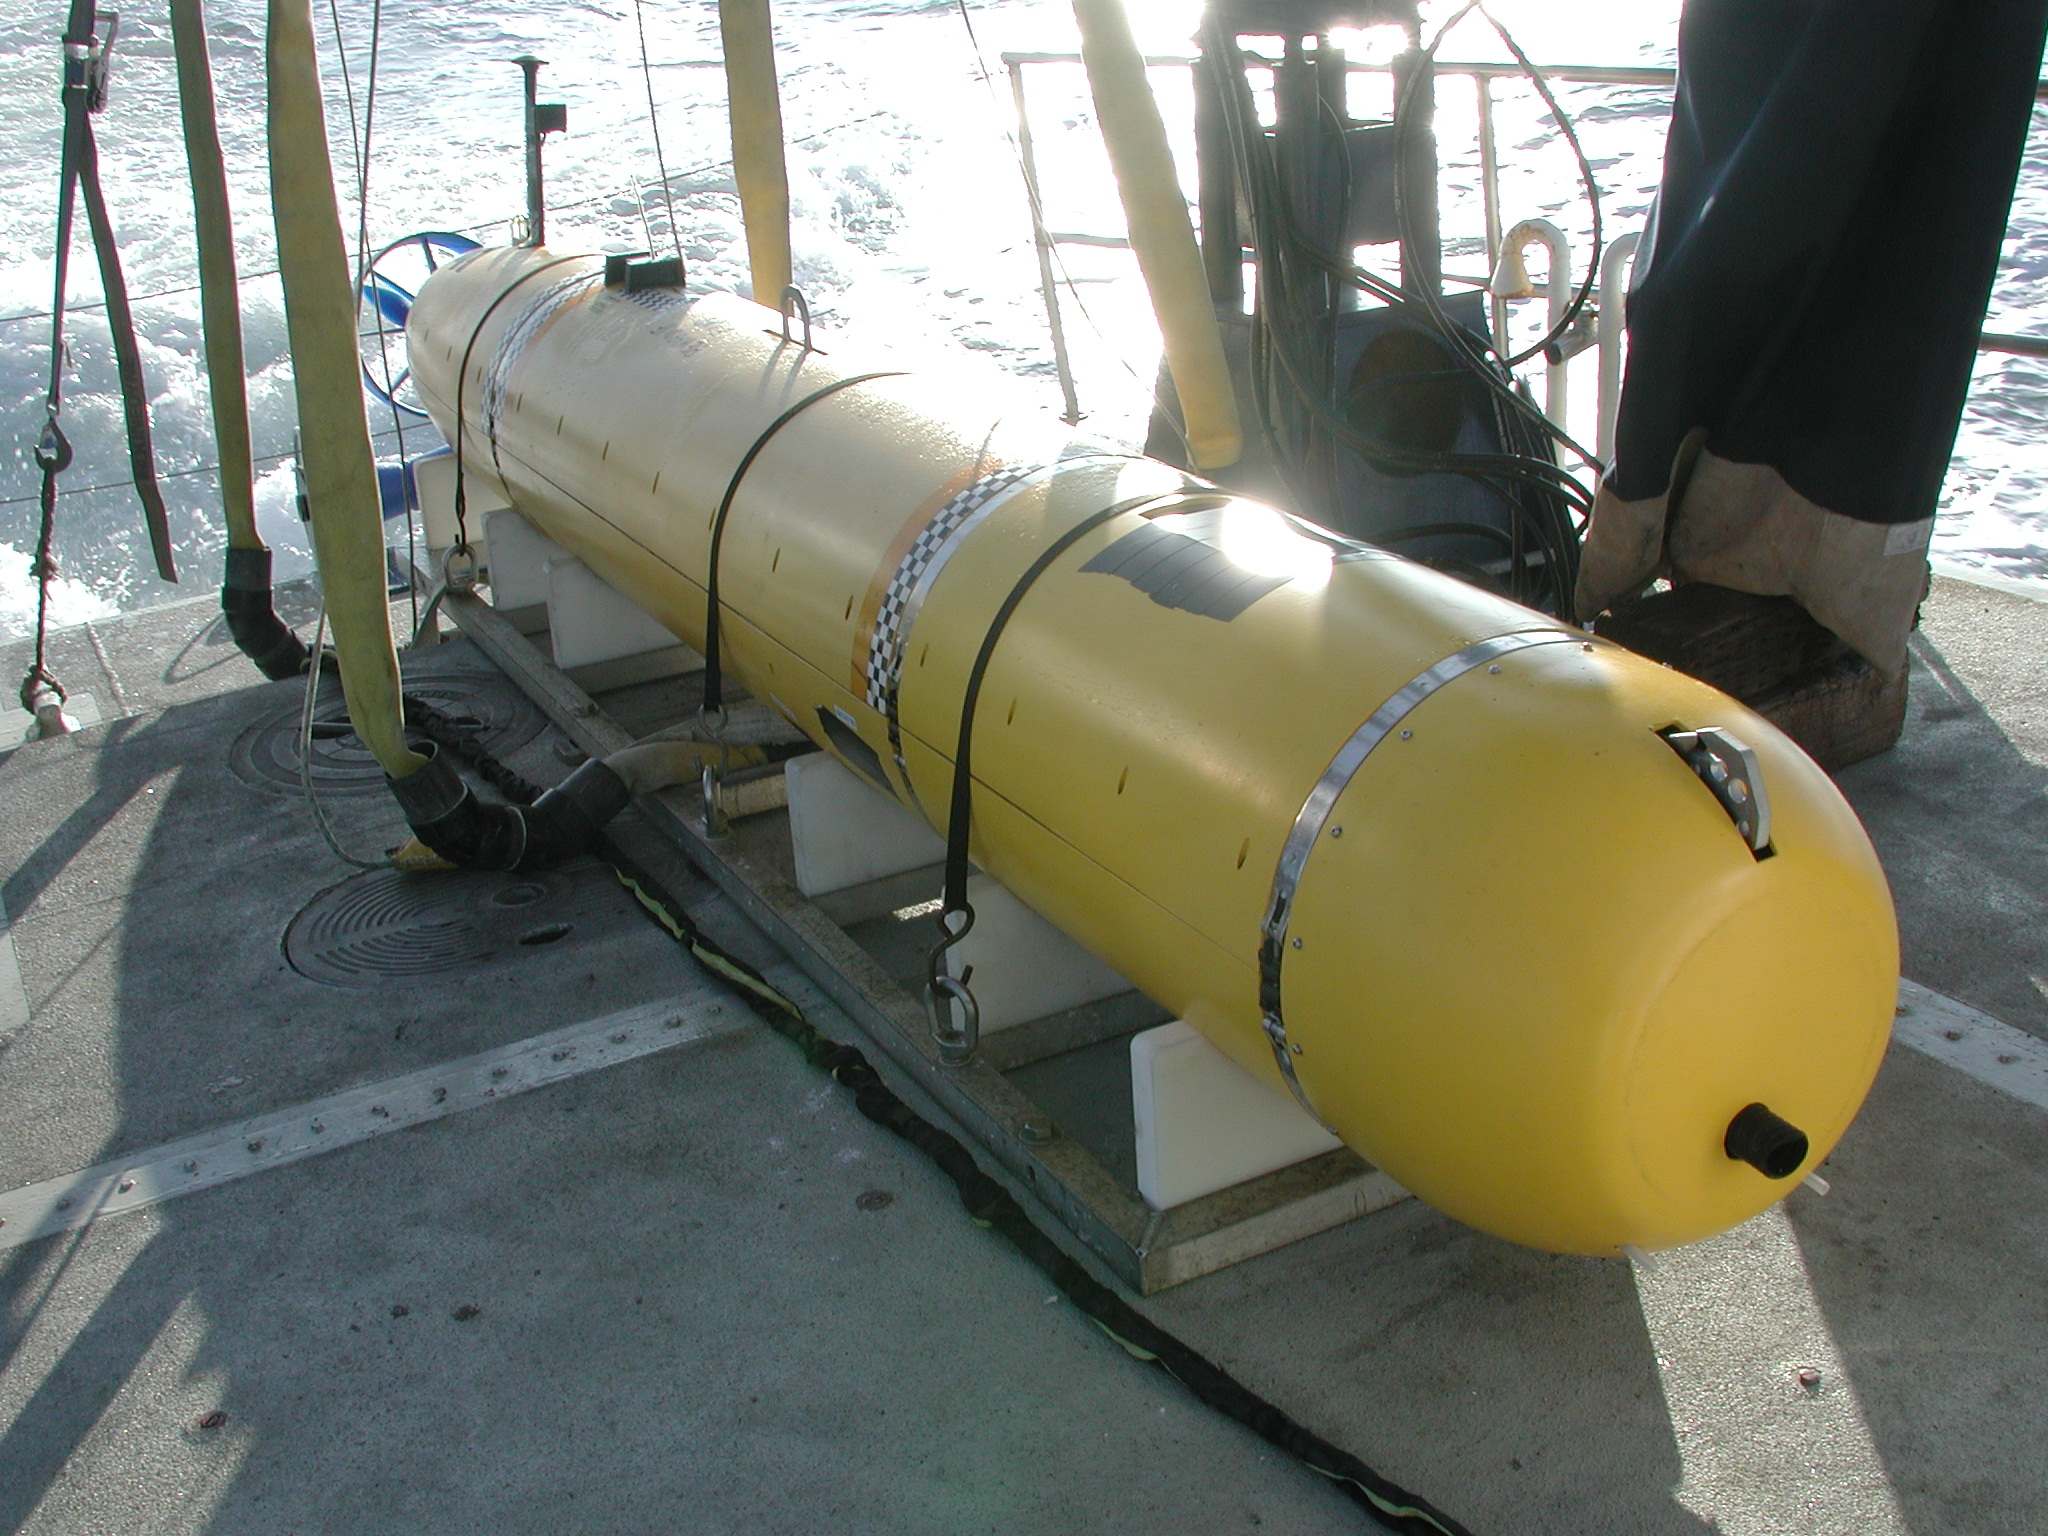
\includegraphics[scale=0.1]{figs/MBARI-AUV.jpg}
  \caption{\small The MBARI \emph{Dorado} AUV on its support vessel
    the R/V \emph{Zephyr}.}
  \label{fig:auv-fig}
  \vskip-0.3cm
\end{figure}

This chapter is organized as follows. We start with some foundational
concepts in our Planning framework in Section
\ref{sec:concepts}. \comment{add others} We conclude with Section
\ref{sec:conclusion}.


\section{Background and Related Work}
\label{sec:related}

% Refer to past work in AUV autonomy as well as robotic autonomy in
% general. This is general purpose and should be a good literature survey
% for robotics and AI.

A distinct problem in Marine Robotics has been the use of the
overloaded term 'autonomy'. Not only does the notion transcend
different disciplines within engineering in this domain (e.g. the
Control Engineering community sees it distinctively from those in AI)
but users of marine platforms in oceanography as well as in maritime
defense conflate the methodology of use (tethered vs. untethered) with
their control. In this chapter, our notion of 'autonomy' deals
explicitly not only with the notion of dealing with the \emph{sense,
  plan and act} paradigm, but also the need to perform
\emph{computational search} between different action outcomes, an idea
central to the field of AI. Consequently, our literature survey here
is targeted towards a more focused and (to this chapter) relevant part
of the field of computation.

With few exceptions, most AUV control systems have been variations of
reactive approaches.  Typically, waypoint-based pre-defined mission
designs are uploaded to the AUV; specialized code fragments called
\emph{behaviors} are designed for the specific mission and a choice of
behaviors for the mission are used on the computational stack
\cite{bellingham94}. Swapping in and out of these behaviors using
conditionals or cleverer and quantitative approaches such as
\cite{Benjamin:2004} forms the basis for adaptation and safety in the
vehicle. Where such swapping does not aid adaptation, individual
behaviors are tweaked to generate some measure of responsiveness to
the surrounding environment \cite{yanwu08} to generate interesting
observations for oceanographers, yet technically naive in terms of
scalability and systematicity. \cite{Benjamin2006} is clear about the
\kcomment{extent} of adaptation in stating:

{\footnotesize
  \begin{quote}
\small \emph{The primary difficulty often associated with behavior-based control
concerns action selection - namely how to ensure the chosen action
really is in the best overall interest of the robot or vehicle.}
\end{quote}
} 

Such techniques have proved their mettle in the first round of use of
AUVs; they've provided operators a simple way to handle control
complexity of the vehicle while returned data at far higher resolution
than would have been possible using traditional ship-based methods and
at substantially reduced amortized costs of platform operation and
ownership over multiple years. AUV operators and clients for their
data products have reasons to be well satisfied with results thus
far. However, as hardware and more cost-effective sensors become more
robust to the environment and as mission durations increase (as
demonstrated by glider experiments such as \cite{rucool11}), sustained
presence in the ocean requires the ability to deal with off-nominal
conditions, that balances the needs of high-level mission management,
low-level navigation, instrument control and detection of unstructured
and poorly understood phenomena. Earlier reactive methods are unable
to perform such a balancing act without skewering the foundations of
the software development methodology leading to code bloat or worse.
\cite{carreras06} provides a good overview of AUV control
architectures essentially based on reactive control methods.

Deliberative techniques for robotic control on the other hand
contrast in providing a distinct set of advantages:

\begin{enumerate}

\item action selection is driven axiomatically based on a systematic
  assessment of a range of causal conditions. An action is selected
  for instantiation only when there is causal support in the form of a
  constraint in a deterministic model of the vehicle's operation.

\item the system is goal directed which forms an objective towards
  which the system is expecting to converge providing a foci in action
  selection.

\item scaling to different (computational) problem size is dependent
  on incremental model building rather than being concerned about
  nuanced interactions between behaviors.

\item systematic software engineering methodologies such as spiral
  development \cite{boehm86} can further be used for scaling up the
  task as demonstrated by \cite{DS1report}.

\item when interactions between actions and/or behavior fragments do
  (and must) occur there are explicit constraints encoded in the model
  that must be computationally satisfied contrasting with carefully
  crafted strategies to instantiate behaviors on a stack. Such
  explicit recording of constraints in the model in turn aids
  long-term software maintenance and sustaining engineering.

\end{enumerate}

\begin{figure}[!t]
 \centering
 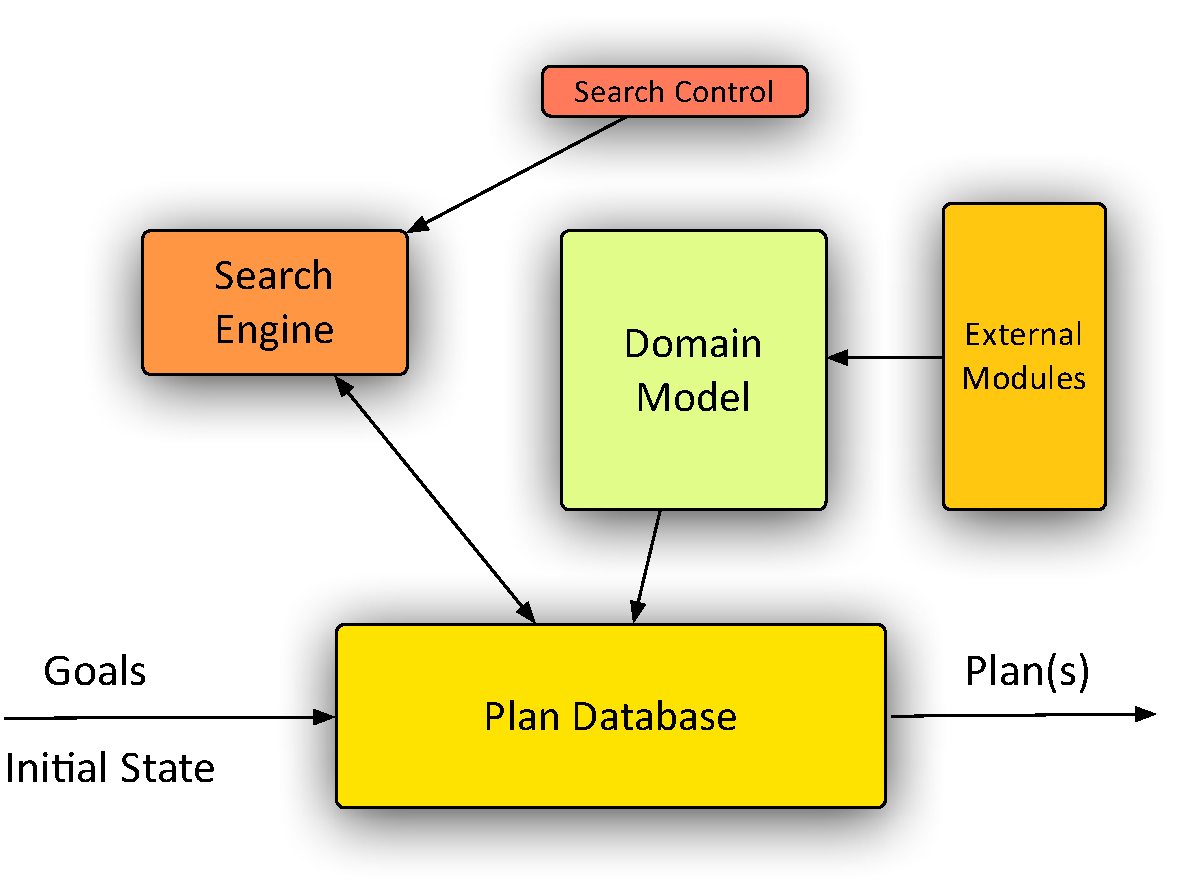
\includegraphics[scale=0.4]{figs/planner-arch.pdf}
 \caption{\small A general architectural block diagram for an AI based
   Planner.}
 \label{fig:planner}
\end{figure}

Traditionally generalized planning has been considered computationally
intensive (the general planning problem can be worse than NP-complete
\cite{ghallab04}). A major reason for this belief had to do with the
role of the planner (which was assumed to be generative) and its place
in the architecture (infrequently called to re-plan the \emph{entire}
mission in off-nominal conditions) within a \emph{sense-plan-act}
paradigm. This can limit the reactivity of a robot especially when the
environment could change at a rate faster than the planner can plan.

The architecture of a typical AI planner is along the lines of
Fig. \ref{fig:planner}. Given a \emph{domain model} which encodes the
platform constraints in a higher-level language, an \emph{initial
  state}, a high-level objective or end \emph{goal}, the \emph{plan
  database} (or \texttt{plandb}) is where all assertions are tracked
and maintained. Theorem proving in the form of satisfaction of axioms
embodied in the domain model occurs within the \texttt{plandb}. It is
the job of the \emph{search engine} to provide the inferential
mechanism for state space exploration potentially aided by heuristics
encoded for \emph{search control}. In some complex domains
\cite{mus98} \emph{external modules} can provide additional domain
expertise which can augment the model. The end result is plan
formulation using a multitude of approaches either using forward or
backward search or using more generalized \emph{partial order} methods
\cite{ghallab04}.


There are costs associated with such inference based control which are
not inconsequential. Foremost among them is the steep learning curve
that comes with the design of the domain model. With limited support
tools necessary for knowledge capture and design of the constraints
often in stylized higher-level languages (see \cite{NDDL} for an
example), it requires the modeler to think in alternative ways to do
problem solving. More importantly it is often necessary for the
modeler to be exposed to the internal representation of the planner
and how it performs search. The level of expertise is often well above
what would be expected of a typical well-rounded Computer Science
graduate student. Yet in our experience, the cost of model design in
such systems, is well balanced against the cost of re-engineering new
mission scripts for new deployment in more ``classical'' script-based
controllers.

However this is mild criticism given the end benefits and the
scientific and engineering goals associated with adaptive and
persistent observation for marine robots whether for civil or military
applications. Given the general problem-solving nature of such
deliberative systems, there is also a substantial overall benefit for
the field of robotics.

\subsection{Evolution of AI-based Robotic Planning: A Necessary Digression}
\label{sec:related:robotplans}

Planning and plan execution are not new to the overall field of
robotics. Early motivation of building computational mechanisms for
decision making were intended to be deployed on robotic devices by
very definition. The seminal volume \cite{computersthought} very
clearly articulates how physical manifestation of robots could be
controlled by task planning and execution. The very first planner
\cite{green69} was an exercise in computational theorem proving with
early state space planners popularized by \texttt{STRIPS}
\cite{strips71} dominating the academic landscape. An early
demonstration of planning as a situated agent\footnote{\kcomment{By
    \emph{situated} we emphasize that an agent is embedded within a
    physical robot.}} was the highly influential \texttt{Shakey} the
robot \cite{shakey84}. Subsequent work driven largely by defense
funding in the United States sequestered the discipline in academic
labs principally applied for algorithmic development and if embedded
then in testing within the confines of \kcomment{structured} indoor
settings. The leap to applying them for real world problem solving is
relatively new and driven largely by NASA applications pioneered by
\cite{mus94,mus98, jonsson00, rajan00, chien05, bresina05}.

The dominant approach for building agent control systems utilize a
$3$-layered architecture (see \cite{gat98} for a well thought out
rationale \kcomment{and survey}), notable examples of which include
\texttt{IPEM} \cite{AmbrosIngerson88}, \texttt{ROGUE} \cite{Haigh98},
the LAAS Architecture \cite{alami:1998p820}, the Remote Agent
Experiment \texttt{RAX} \cite{mus98} and the Autonomous Spacecraft
Experiment \texttt{ASE} \cite{chien99} (see \cite{Knight01} for a
survey). 

Representationally, the first paper on managing time systematically
within AI Planning frameworks was \cite{dean87}; subsequent efforts by
Boddy and others \cite{Dean88,Boddy93} refined the notion of using a
temporal database and the conceptualization of temporal
intervals. Using these concepts Muscettola and others \cite{mus92,
  ghallab94, laborie95, cesta96} developed the notion of plan/schedule
envelopes using the notion of state variable instantiated
timelines. Simultaneously work by Dechter et.al \cite{dechter91}
resulted in efficient temporal constraint propagation which
systematically defined the notion of Simple Temporal Networks (STNs)
and path and arc consistency algorithms. This work neatly put together
earlier efforts by Mackworth and Freuder \cite{mackworth77, mack85}
and the Constraints community on propagation algorithms. In parallel
work in the UK, resulted in the design of \texttt{O-Plan}
\cite{currie91}, which leveraged the notion of constraints and metric
time, but within a Hierarchical Task Network (HTN) representation.
These efforts were soon after Vere’s paper on planning and time
\cite{vere83} which had a profound effect on the AI Planning
community. In particular the work of Muscettola \cite{mus94} was
embraced by NASA for telescope scheduling. Around the same time
period, researchers at LAAS came up with an architecture
\cite{alami:1998p820} which encapsulated the \texttt{IxTeT} planner
\cite{ghallab94} \kcomment{which dealt with time and resources}. It
featured advanced concepts for a temporal planner with the notion of
chronicles, plan recognition for partial plan fragments and early use
of systematic resource constraints. % Development on \texttt{IxTeT} has
% continued albeit at a slower pace with the contribution of various PhD
% students’ thesis.

\subsection{The Remote Agent Experiment and beyond}
\label{sec:rabeyond}

While \texttt{HSTS} \cite{mus94} was being implemented as a
ground-based planning tool for decision support for US based space
observations (EUVE and Cassini) \cite{mus95}, the opportunity to fly
onboard NASA’s New Millennium Deep Space $1$ came about. The design of
the Remote Agent Experiment \texttt{RAX} \cite{pell97, bernard98,
  pell98, mus98, DS1report, rajan00, jonsson00} was a direct off-shoot
of this effort where \texttt{HSTS} (written in LISP) was flown on
board and successfully commanded the spacecraft for a week in May
1999\footnote{This was the first (and to our knowledge only) software
  ever to been written in \texttt{LISP} to be flown in space.}. There
were a number of significant software engineering lessons learned with
the HSTS technology as \kcomment{implemented} for the RAX
\kcomment{experiment}:

\begin{enumerate}

\item Constraint-based representations were not only sufficient for
  plan synthesis, but valuable during debugging and development as a
  means of building a viable domain model.

\item Domain models when separated from the search engine as
  articulated by the model-based approach \cite{williams96a} ensured
  that sufficient effort would be targeted on human validation of the
  model building phase while ensuring that search engine stability
  across applications and domains resulted in lower cost to deploy.

\item Flexible temporal representation generating a range of plans as
  against a single plan, were robust for \kcomment{robotic} plan
  execution.

\item If planning and execution were disconnected (as in
  \texttt{RAX}), dispatchabilty \cite{mus98a} and controllability
  \cite{morris00} issues within temporal plans need be addressed. In
  \texttt{RAX}, a post-processing step was added to counter these
  effects. It was clear that execution needed access to the planners
  database and be able to propagate execution time constraints prior
  to command dispatching.

\end{enumerate}

It was with the demonstration of \texttt{RAX} $65$ Million miles in
outer space, that temporal reasoning using \kcomment{planning} methods
came to the forefront of AI Planning for situated agents. Lessons
learned from \texttt{RAX} led to the development of \texttt{IDEA}
\cite{mus02,mus04,Dias:2003ua,mus06} with the central theme of using
planners collectively for problem solving. Another critical theme was
iteratively and incremental plan repair of an anytime plan
\cite{Zaimag96} as proposed by \texttt{CASPER} \cite{chien00}.

This last lesson in particular had a lasting impact with the
observation that planning and execution are strongly
inter-related. This core concept was behind the next generation of the
Remote Agent, called \texttt{IDEA} (Intelligent Deployable Execution
Agents) where planning and execution were \emph{intertwined} within a
single domain model that spanned the most abstract (for high-level
planning) to the least (for diagnosis). \texttt{IDEA} \cite{mus02,
  mus04} agents were expected to interact to achieve plan formulation;
however there was no systematic framework for formally governing these
interactions. \texttt{IDEA} was also computationally heavy and
required substantial effort to customize for an application domain. It
did move to a retooled version of \texttt{HSTS}, called \eu
\cite{frank2003, barreiro09} while being ported to the C++ language.

While \texttt{IDEA} was being deployed as a coordinating executive for
earth analog rover deployments \cite{wetter05} a separate development
was undertaken to deploy the \eu planner for NASA’s Mars Exploration
Rovers (MER) mission. The \texttt{MAPGEN} (Mixed-initiative Activity
Plan GENerator) planner \cite{bresina03, aichang04, bresina05,
  bresina05a} as a decision support tool in the mixed-initiative mode;
\texttt{MAPGEN} continues to be used to this day to command the twin
rovers on the Red Planet. % While EUROPA2 was not
% designed as an embedded planner, NASA undertook a bottom-up
% re-implementation of the planner and substantially increased its
% performance. EUROPA2 was then released as open source to the AI
% community at large [Europa].

The Autonomous Sciencecraft Experiment (\texttt{ASE}) \cite{chien99,
  chien03} was another autonomy demonstration in space, this time for
a more observable vehicle, the EO-1 in Earth orbit. It encapsulated a
classical 3-layered architecture like \texttt{RAX}. Goals could not
only be sent by a ground segment, but also by an onboard science
driver which could encapsulate a range of Machine Learned feature
detectors which could trigger the planner. However \texttt{ASE} was
not an integrated system; the \texttt{CASPER} planner \cite{chien00}
would generate plans which were executed by a separate commercially
available rule-based system \cite{icl}. \texttt{CASPER} demonstrates
what is called as a \emph{continuous} paradigm for incremental
planning and iterative plan repair; this methodology takes the overall
mission plan and selectively plans \kcomment{for the} near-term at a
more detailed level.
% The system also uses iterative-repair as a way to fix
% plans; however this too is derived from a model of the mission and
% spacecraft constraints which allow simple reconfiguration modes
% towards replanning. 
Robust software engineering is also not an important aspect targeted
by \texttt{ASE} given the disparate models between the planner and the
rule-based executive. With such a system, real-time updates from the
environment could not be accommodated since the planner is a
monolithic computational environment. The rate of updates from the
science drivers is roughly \kcomment{on} the order of an earth orbit
on the EO-1 vehicle. As a result, the \texttt{ASE} is only an
incremental update on \texttt{RAX} and is not suitable for domains
where complex automated reasoning and asynchronous environmental
observations need to be factored in deliberation.

\texttt{TCA} \cite{simmons94} another framework for robot control and
has similar motivations to \texttt{RAX} and \texttt{ASE}. Reactivity
and deliberation are also key to \texttt{TCA} \kcomment{along with} a
systematic approach to development led to its design. However it
suffers from three key weaknesses. First it has a weaker
representational framework of Task Trees which require representation
of tasks within cleanly formulated hierarchies. Constraints between
branches within a task hierarchy are allowed; timing between leaves of
different trees is however not possible. Second, its temporal
framework does not deal with flexibility; time points are fixed and
while partial orders are possible, it does deal with execution time
uncertainty. Third, while \texttt{TCA} shares the notion of using
domain expertise of different planners, it does so thru a centralized
message passing mechanism. While this allows disparate code-bases to
talk to each other \kcomment{through} IPC (\kcomment{an} inter-process
communication or message passing mechanism), failure in the
centralized controller is tantamount to a system crash.

The \texttt{ReSSAC} project at ONERA \cite{teichteil07} \kcomment{is
  motivated by} controlling aerial UAV platforms for autonomous Search
and Rescue. Like \texttt{TCA}, the project uses a supervisor to
control planning and at the same time decouples the deliberation and
reactive components from the lower level functional layer. This
deliberate separation is partly because of the use of optimizing MDP’s
(Markov Decision Processes \cite{mdp93}) for planning which uses
probabilistic state transitions to determine the next course of action
based on perceived state. To overcome the typical problem of state
space explosion with MDPs, a local heuristic is used in order to
generate reachable goal states incrementally. This work however does
not deal with metric time \kcomment{and comes} with a modestly simple
model.

\texttt{CIRCA} \cite{musliner95} is an effort to bring decision making
for real-world problems with the augmented need to have
\emph{verifiable} controllers synthesized in-situ to ensure that
\kcomment{during state space exploration}, there are no erroneous
transitions to dangerous states by asynchronously generating
Test-Action-Pairs (TAPs).  These are annotated production rules
consisting of a set of tests (or preconditions) and a set of actions
to take if all the tests return true. TAPs are synthesized and
scheduled by \texttt{CIRCA} and provide a viable way to deal with a
dynamically changing world. \texttt{CIRCA} however differentiates
between reasoning about time and reasoning in real-time with the
implication that reasoning necessarily requires substantial
computation for state space exploration which negates the real-time
(and thus real-world) impact.

A key and early concern that dominated planning was that of
scalability.  The planning cycle in many approaches was \kcomment{(and
  is)} monolithic, often making fast reaction times impractical when
necessary for embedded robotic agents. Many of these systems (which
were $3$-layered) also utilized very different techniques for
specifying each layer in the architecture resulting in duplication of
effort and a diffusion of knowledge.  The work we highlight in this
chapter builds on the approach used by \texttt{IDEA} \cite{mus02,
  mus04} in utilizing a collection of controllers, each interleaving
planning and execution within a common framework. \texttt{IDEA}
however, provided no support for conflict resolution between
controllers, nor did it provide an efficient algorithm for integrating
current state within a controller, relying instead on a possibly
exponential planning algorithm. Efficient synchronization of state in
a partitioned structure is fundamental to making the approach
effective in practice.

Our system, \rxe, the focus of this chapter, is an agent control
structure formally defined as a composition of coordinated control
loops where sensing, planning and acting \kcomment{result} from
concurrent deliberating tasks within a formal framework.  \rx was
designed after carefully evaluating lessons learned from \texttt{IDEA}
to which it owes substantially the notion of partitioned problem
solving. Partitioning in \rx is systematic and methodologically
principled where we manage the information flow within the partitioned
structure to ensure consistency in order to direct the flow of goals
and observations in a timely manner. The resulting control structure
improves scalability since many details of each controller can be
encapsulated within a single control loop.  Furthermore, partitioning
increases robustness since controller failure can be localized to
enable graceful system degradation, making this an effective
\emph{divide-and-conquer} approach to \kcomment{solving} the overall
control problem.

A recent variation of the key idea of such controller composition
derived from \rx is \texttt{ROAR} \cite{degroote11} where lower-level
functional modules that control sensors are organized within a graph
hierarchy. One reason they cite such a structure \kcomment{as being}
essential is in dealing robustly to failure; an off-nominal condition
will allow rapid graph traversal to identify alternative ways in which
sensing tasks can be executed and therefore aiding \kcomment{platform}
responsiveness. % However,
% it is unclear whether to date this system actually deliberates and
% whether it is actually instantiated on a real platform for control.

% ``The whole partition must be accordingly reorganized: this kind of
% construction does not scale well over a large variety of missions,
% missing the objective of a versatile architecture for robots.''

%%% Local Variables: 
%%% mode: latex
%%% TeX-master: "setobook"
%%% End: 


\section{Foundational Concepts}
\label{sec:concepts}

\rx is an adaptive, artificial intelligence based controller and
provides \kcomment{a} general framework for building reasoning systems
for real-world autonomous vehicles. At MBARI \rx is used for AUV
control; another instantiation of the system is being used for control
of a terrestrial personal robot \cite{pr2, Meeussen:2010dn}. The
development of \rx has been targeted at surveying a number of
oceanographic features which are dynamic and spatio-temporally
unpredictable. Typically this requires our AUVs to balance the goals
of spatial coverage while opportunistically following features of
scientific interest and to do so while being aware of its own resource
limitations (\eg the battery state of charge) and overall proximity to
other observational assets for obtaining scientific ground-truth. We
are interested in representational frameworks that allow robots to
pursue long-term objectives while choosing short-term gain and can
gracefully deal with exogenous or endogenous change.

To enable this responsiveness to external observations, the agent has
to be able to synthesize plans insitu and to re-plan without human
intervention. \rx uses a temporal constraint-based planner with a
demonstrated legacy of having flown on NASA space missions. Our
autonomy architecture brings three key innovations for AUV control:
in-situ plan synthesis, the use of flexible plan representations with
a sound theoretical basis and systematic compositional control with
the use of partitioned networks and doing so with a demonstrated
capability at sea \kcomment{for} novel ocean observation methods.

The next few sections will cover \eu in a bottom-up fashion, going
from its \kcomment{general} theoretical framework, to the specific
representation, modeling and algorithms implemented by it.  A brief
introduction to Constraint Programming and Constraint-Based Planning
is provided followed by the specific representation that \eu uses to
undertake Constraint-Based Planning.  Subsequently, we provide an
overview of \eus architecture and how it can be embedded in a planning
application such as \rxe. Finally, \eus modeling, inference and search
mechanisms are covered in detail so that the reader can
\kcomment{appreciate} how \rx can perform \kcomment{deliberation while
  being responsive to events in the real-world}.

\subsection{Automated Planning}
\label{sec:planningfound}

{\scriptsize
  \begin{quote} [Planning] \emph{is an abstract, explicit deliberation
      process that chooses and organizes actions by anticipating their
      expected outcomes. This deliberation aims at achieving as best
      as possible some prestated objectives. Automated planning is an
      area of Artificial Intelligence (AI) that studies this
      deliberation process computationally.} -- from \textbf{Automated
      Planning Theory and Practice} by Ghallab, Nau and Traverso
    \cite{ghallab04}
\end{quote}
}

Planning as an activity is ingrained in human decision-making
\cite{berthoz} and its generalization into a computational framework
demonstrating machine intelligence \kcomment{has for long been}
targeted by pioneers in computer science
\cite{computersthought}. Early work in this context focused on logical
theorem proving by computer \cite{green69} which has formed the basis
of much of the discipline. The emphasis in these early efforts was to
logically derive the existence proof of a trajectory of actions for a
hypothetical robot (moving blocks, chess pieces, furniture etc) to
achieve a specific goal given specific initial conditions. Two
important properties of \emph{Soundness}\footnote{A planning algorithm
  is sound if invoked on a problem $P$ returns a plan which is a
  solution for $P$.} and \emph{Completeness}\footnote{A planning
  algorithm is complete if invoked on a solvable problem $P$ is
  guaranteed to return a solution.} along with derived results for
algorithmic complexity \cite{gareyjohnson,corman} were a defining
cornerstone for understanding how different computational paradigms
could actually be tractable first in simulation and subsequently in
actual robotic platforms. In this chapter our emphasis is to focus on
embedded AI Planning and the execution of plans on an embedded
\kcomment{marine robotic} platform. The techniques we highlight are
general purpose as noted in Section \ref{sec:intro}.

\begin{figure}[b]
\centering
  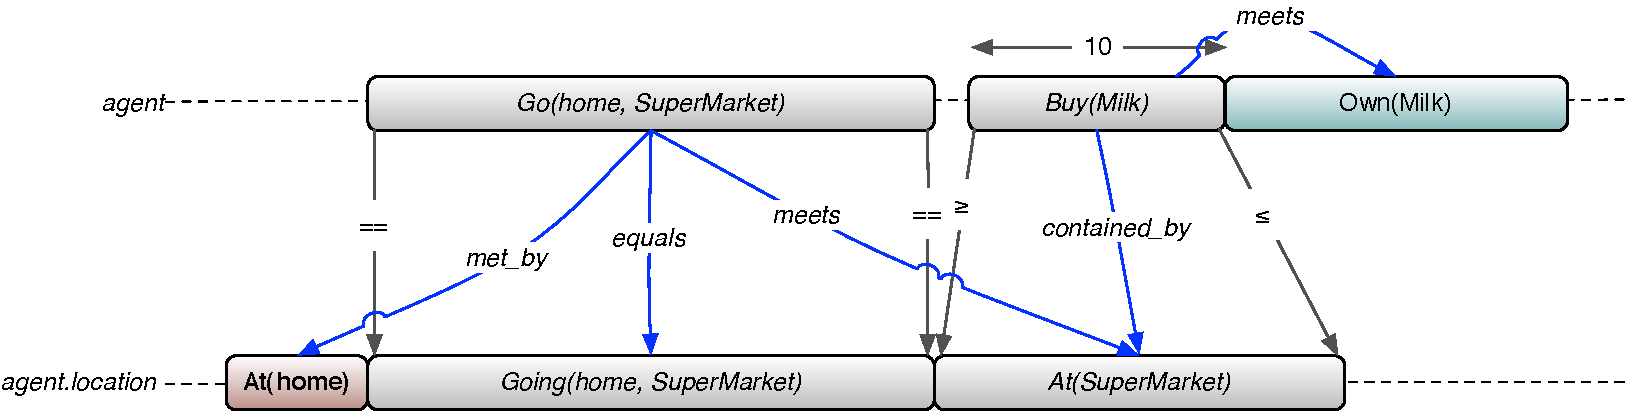
\includegraphics[scale=0.45]{figs/shopping_europa.pdf}
  \caption{\small A potential plan for a robot shopping for groceries.}
\label{fig:shop:shopping}
\end{figure}

To articulate the fundamentals of automated planning briefly and use
that to motivate the mechanisms we use in our specific form of
planning we start with an example.

{\small
  \begin{quote}
    In the near future, a personal robot sets out to buy a gallon of
    milk. This involves a number of tasks: obtain keys, obtain wallet,
    start car, drive to store, find and obtain milk, purchase milk,
    etc.  The embedded planner has to have a ``model'' of the world in
    which it 'lives' and has to use the task primitives in this model
    to structure the actions so it achieves its goal. Constraints
    control when certain tasks can or cannot occur. For example the
    robot must obtain the keys and wallet \emph{before} driving to the
    store and pick up the milk \emph{before} purchasing it.
\end{quote}

For such a robot the milk buying plan at the store might look like
that shown in Fig. \ref{fig:shop:shopping}.

At the core of the \rx framework, is the deliberation engine, \eue,
which has a rich legacy from NASA missions \cite{mus98,rajan00,
  jonsson00,aichang04, bresina05}. \eu is a versatile Constraint-based
Temporal Planner which continues to be deployed on a diverse set of
applications including recently, planning for the International Space
Station \cite{barreiro09}. We first motivate this section with some
problem domains this planner has handled.

\paragraph{} {\em Constraint Satisfaction}: A canonical problem in
dealing with constraints is the $N$-Queens problem in which chess
queens must be placed on an $N \times N$ chessboard so no queen can
attack the other. 

If we define $N \times N$ variables Q$_{rc}$, $r \in [1,N]$, $c \in
[1,N]$, Q$_{rc} = 1$ if cell $r,c$ in the chessboard is occupied by a
Queen, $0$ otherwise. Then the following constraints need to be
satisfied:

\begin{eqnarray*}
 Sum(Q_{rc}) & = & \left\{
   \begin{array}{l l}
     1 & \forall r \quad \mbox{(only one Queen per row)}\\
     1 & \forall c \quad \mbox{(only one Queen per column)}\\ 
   \end{array} \right. \\
Sum(Q_{r+i,c+i}) & = & 1\\
Sum(Q_{r-i,c-i}) & = & 1 \qquad \mbox{(only one Queen on each diagonal)}\\
\end{eqnarray*} 

The problem can be solved by finding assignments for all variables
Q$_{rc}$ that satisfy the above constraints. Fig. \ref{fig:nqueens-2}
is a solution found by \eu using a compact version of that formulation
and a specialized search procedure.

\begin{figure}
\centering
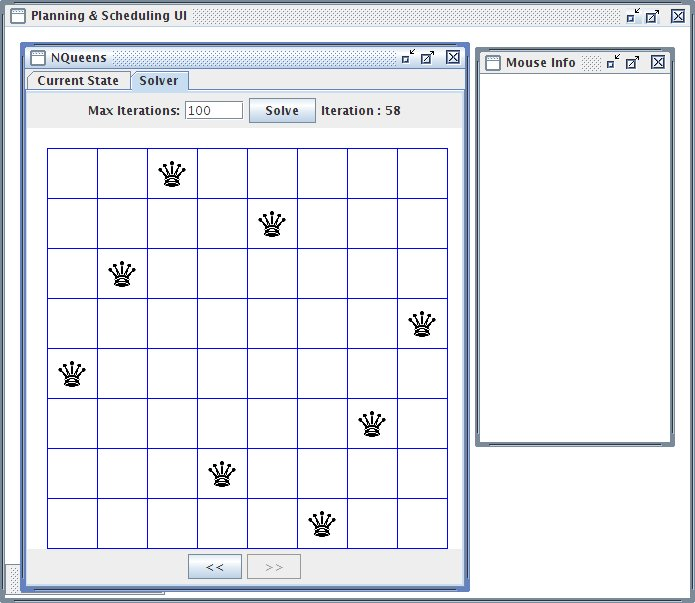
\includegraphics[scale=0.3]{figs/Example-NQueens1.jpg}
\caption{\small An $N$-Queens solution generated by \eu}
\label{fig:nqueens-2}
\end{figure}


\paragraph{} \textit{Scheduling}: The Resource Constrained Project
Scheduling Problem (\texttt{RCPSP}) \cite{Bruckera99}, consists of a
set of activities that must be scheduled in a way that satisfies
minimum and/or maximum temporal separation constraints. The activity
schedule must also respect fixed limits on the availability of
resources required to perform each activity. In addition to satisfying
temporal and resource constraints, it is common for the user to want
to minimize makespan \cite{ghallab04} so that the entire project is
finished as early as possible. Fig. \ref{fig:rcpsp-1} shows an example
of a a solution provided by \eu for an \texttt{RCPSP} instance with
$10$ activities, $5$ resources and $30$ temporal constraints.

\begin{figure}[t]
\centering
\subfloat[\small A \eu solution to an \texttt{RCPSP} \cite{Bruckera99}
  problem.]{\label{fig:rcpsp-1}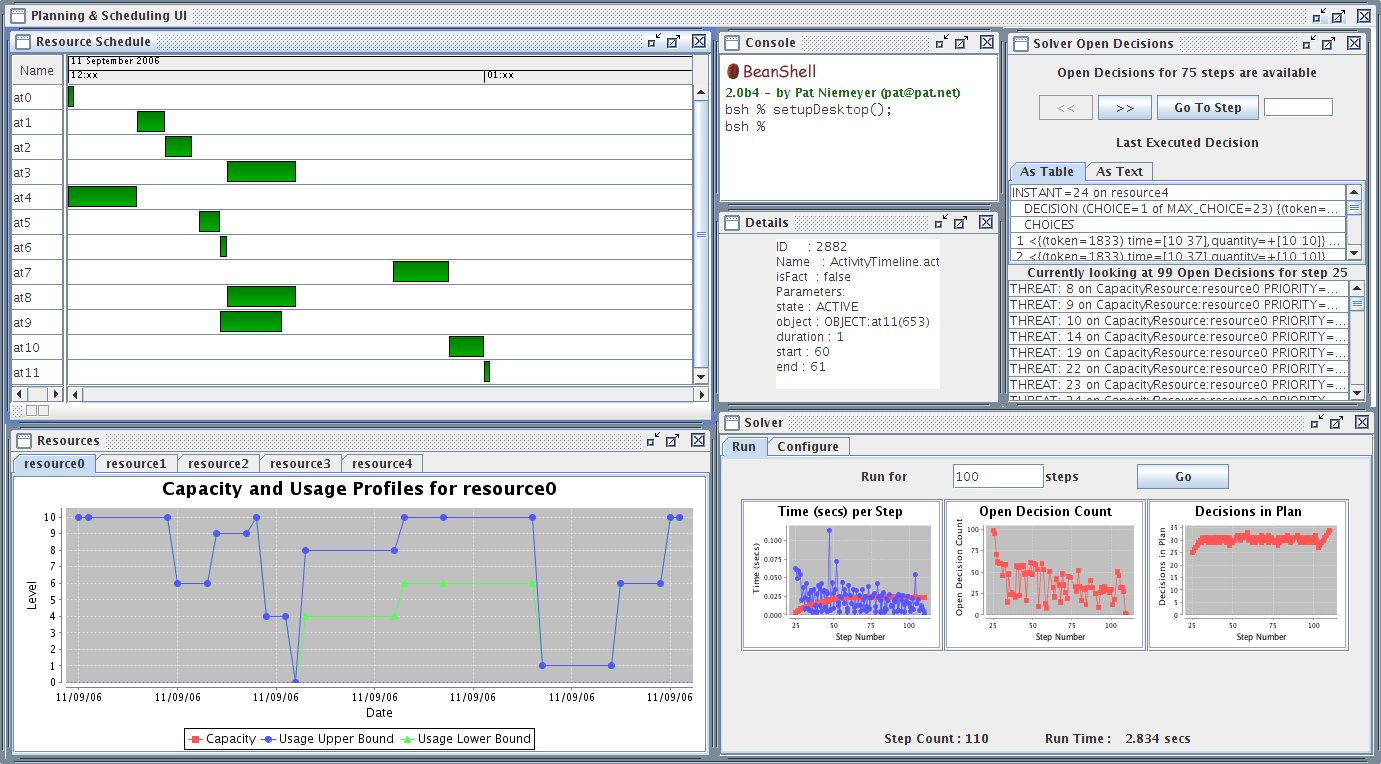
\includegraphics[scale=0.25]{figs/Example-UBO0.jpg}}\qquad
\subfloat[\small A \eu solution to a shopping agent problem domain where
  the agent needs to buy Bananas, Milk and a Drill.]{\label{fig:shopping-1}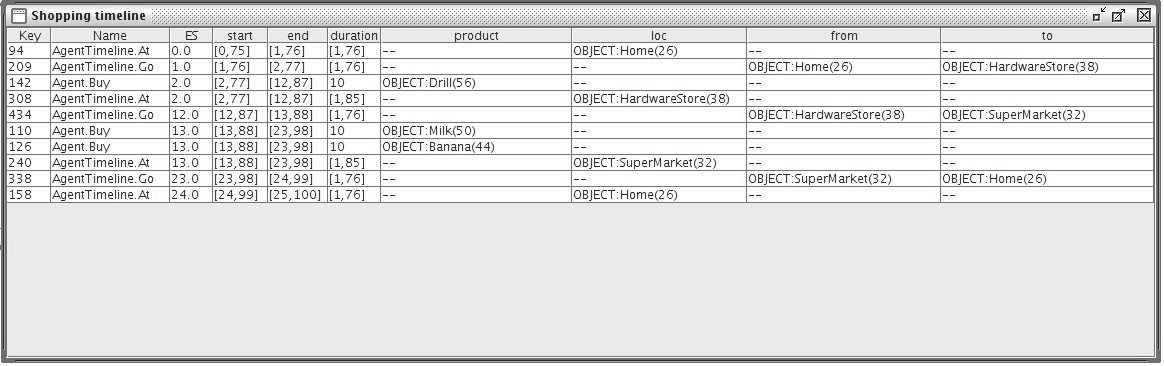
\includegraphics[scale=0.3]{figs/Example-Shopping0.jpg}}
\caption{\small \eu based solutions to scheduling and planning problems.}
\end{figure}


\paragraph{} \textit{Planning}: The Shopping Agent Problem
\cite{russelnorvig} is a variation of the problem with which we
started this chapter.  An agent needs to purchase a set of products
(milk, drill, etc) that are available at specific locations
(supermarket, hardware store, etc). The agent is subject to temporal
(must complete tasks by specific deadlines) and resource (fuel,
carrying capacity, etc) constraints and it needs to synthesize actions
that need to be performed to find and acquire the required items, as
well as when to perform each of those actions.
Fig. \ref{fig:shopping-1} shows a solution produced by \eu for such a
problem instance.

As the examples above show, a Planning problem (actions to achieve a
goal) may embed a Scheduling problem (what resources are necessary to
achieve stated goals) and both Planning and Scheduling may embed a
Constraint Satisfaction problem.  The relationships between Planning,
Scheduling and Constraint Satisfaction have been examined
\cite{smith00} and have lead to use of constraint reasoning in \eu as
a core building block.

\subsection{Constraint Programming}
\label{sec:europa:cp}

Constraint Satisfaction Programming (also known as Constraint
Programming or \textsf{CP}) is \kcomment{an AI} discipline that
provides a generic framework for representing, solving and making
logical inference on constraints. A complete treatment of this
discipline is given in \cite{marriott98,apt03} with concise
introductions provided in \cite{bartak99,lustig01}.

A constraint programming problem consists of a set of variables $V=
{x_1,..,x_N}$, where each variable takes values from a domain
$d_1,..,d_N$; in this chapter we will deal only with discrete and
finite domains. Given a defined conjunctive set of constraints
\kcomment{\cite{gen87}} on the variables: $C=\{c_1(x_1,..,x_N), ...,
c_K(x_1,..,x_N)\}$, the objective is to find one or more value
assignments to $V$ where all constraints are satisfied. To solve a
problem, \textsf{CP} techniques use logical inference to perform
Constraint Propagation, which consists of two operations:

\begin{enumerate}

\item \textbf{Bounds propagation} inferring upper and lower variable
  bounds. For example, from the constraints $x_1 + x_2 \leq 2$ \& $x_i
  \geq 0$, we can infer $[0,2]$ bounds for $x_1$ and $x_2$.

\item \textbf{Domain reduction} inferring a valid set of values for a
  variable.  For example, for constraints
  \texttt{allDifferent}($x_1,x_2,x_3$), $x_i \geq 0$ \& $x_i \leq 4$,
  if $x_1 = 1$ and $x_2 = 3$ we can infer that the valid and reduced
  domain for $x_3$ is $\{2,4\}$.

\end{enumerate}

A set of constraints and variables that describe a problem domain are
typically represented as a \emph{Constraint Network}, where the
variables are nodes and constraints are arcs between the variables. A
pair of variables $x$ and $y$ is said to be \emph{arc consistent} if
for every value in $x$'s domain, there is a value in $y$'s domain that
is consistent with all the constraints that connect $x$ and $y$.  A
naive approach to ensuring arc consistency consists of cycling through
all the variable pairs and performing constraint propagation until
there are no variable domain changes. The \texttt{AC-3} algorithm
\cite{mackworth77}, a popular implementation, improves over the naive
approach by ignoring constraints whose variables were not affected
since the last iteration. Fig. \ref{fig:constraintnet} shows a set of
constraints on $3$ variables ($x$, $y$ and $z$) represented as a
constraint network and their domains before arc consistency is
enforced.  After the \texttt{AC-3} algorithm is executed, the domains
for the variables would be pruned to x=$\{2$\}, y=$\{2$\}, z=$\{2$\}.

\begin{figure}[!t]
\centering
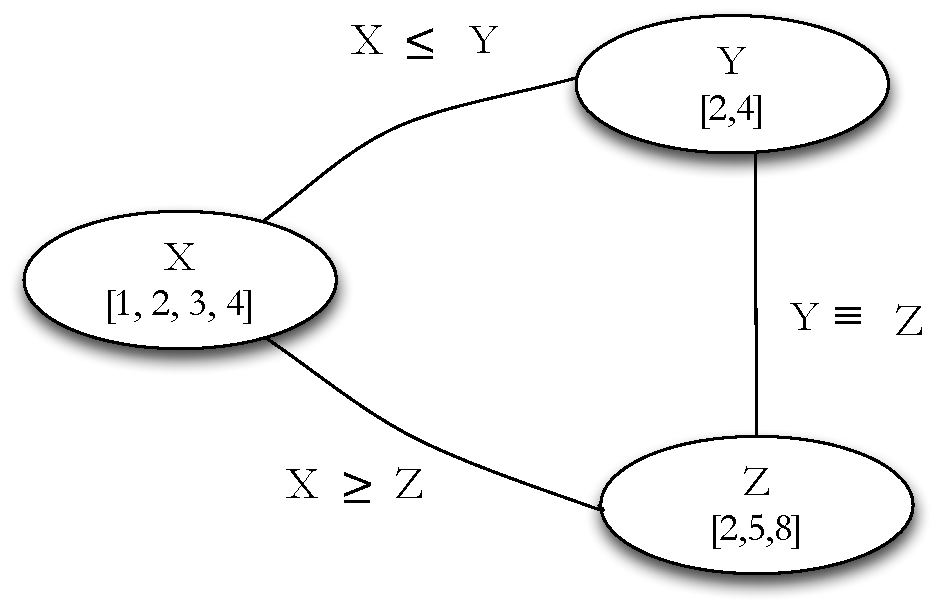
\includegraphics[scale=0.3]{figs/constraint-net.pdf}
\caption{\small Variables and Constraints represented as a Constraint
  Network \kcomment{before arc consistency is enforced}.}
\label{fig:constraintnet}
\end{figure}

Arc Consistency and other more stringent consistency definitions can
be used to efficiently prove that a \textsf{CP} problem is
\emph{unsatisfiable}. However, they generally cannot prove that a
\textsf{CP} problem is satisfiable and provide specific variable
assignments that constitute solutions. To do so, search algorithms
like global backtracking \cite{hooker05} or local search are used.
These use consistency as an efficient way to prune the search space
\cite{cp06}. In theory, solving a \textsf{CP} problem is NP-Hard
\cite{ghallab04}, but often in practice \kcomment{heuristic methods
  provide viable ways to generate efficient solutions}.

\textsf{CP} is usually implemented as part of a programming language
and constraints are usually represented as objects \cite{puget95}. Any
constraint that the user is able to reason about can be introduced
into the system and as long as the constraint propagation protocols
specified by the host \textsf{CP} system are enforced, it will be
indistinguishable from any other "primitive'' \textsf{CP} constraint,
such as $\leq$ or $\geq$.


\subsection{Constraint-Based Planning}
\label{sec:europa:cp}

The most common planning formulations use propositional
\kcomment{logic}, where the state of the world is represented by a set
of propositions (statements that can be true or false), and operators
change the truth values of these propositions \cite{gen87}. Although
these formulations are powerful \kcomment{for descriptive semantics}
in automated planning, there are classes of problem domains that are
difficult to represent. In particular, it is hard to represent time,
resources, mutual exclusion and concurrency.  Constraint Programming
is a framework that lends itself well to represent and reason about
these elements \cite{ghallab94} with the consequence that there has
been substantial effort in building automated planners that
\kcomment{leverage} \textsf{CP} techniques.  The most common approach
in constraint-based planning has been to encode the entire planning
problem as a \textsf{CP} problem, where action choices and
relationships are represented as variables and/or constraints
\cite{do01,vanbeek99,vossen99,wolfman99}.  The advantage of using a
pure \textsf{CP} formulation is that standard solvers can be then used
to solve the planning problem. However, this approach also has
significant drawbacks:

\begin{enumerate} 

\item Given that action choices and relationships (rules) are
  expressed through variables, the domain descriptions that result
  from this approach are not intuitive and therefore difficult to
  understand and debug.

\item If the structure of a planning model (actions, conditions,
  effects, dependencies at the action level) is not explicitly
  maintained by the \textsf{CP} planner, the search algorithms are
  deprived of critical information to make better decisions. If that
  structure is maintained (for instance, by internally marking
  variables that represent action choice and relationships between
  actions), it is still hard to write search algorithms as any
  planning-specific insight has to be translated into the \textsf{CP}
  representation of variables and constraints.
  
\end{enumerate}

These drawbacks have been addressed by a number of frameworks like
\texttt{Descartes} \cite{joslin95,joslin96}, \texttt{IxTet}
\cite{ghallab87,lemai04} and \texttt{CAIP} (Constraint-Based Interval
and Attribute Planning) \cite{mus94,frank2003}.  They take advantage
of a \textsf{CP} representation to deal with time and resources,
\kcomment{while} maintaining an explicit representation of the
elements relevant to planning (action choices, causal relationships,
etc). This combination results in a planning approach that can deal
with the \kcomment{kind} of constraints found in real-world problems
while allowing for intuitive problem descriptions and a natural way to
express search algorithms and heuristics. \eu is one such
implementation of the \texttt{CAIP} framework, \kcomment{others
  include \cite{chien00, iaai-CestaCFO09}}. In \eu planning problems
are specified in terms of:

\begin{description}

\item[\textbf{Intervals}:] entities that have a temporal scope (that
  is, a beginning and an end in time) and a set of
  attributes. Intervals are used to represent actions and states in
  the planning domain.

\item[\textbf{Variables and Constraints}:] Variables represent Interval
  attributes and constraints enable a direct representation of
  temporal, resource and any other restrictions that a valid plan must
  comply with.

\item[\textbf{Domain Configuration Rules}:] This is an explicit
  representation of the conceptual relationships between actions and
  states in the problem domain, for instance, for a Shopping Agent to
  be able to purchase a product, it must be at a location where the
  product is available.

\end{description}

To generate plans, the \texttt{CAIP} framework uses a plan-space
search approach \cite{ghallab04}, where a \emph{partial
  plan}\footnote{\kcomment{A partial plan is a subsequence of a plan
    which can be refined into a plan structure.}} is evolved until all
open goals are achieved and all inconsistencies are removed. The
specific search algorithm used by \eu will be covered in
\kcomment{further} detail below.


%%% Local Variables: 
%%% mode: latex
%%% TeX-master: "setobook"
%%% End: 


\section{\eu Basics}
\label{sec:basics}

\paragraph {A brief note on \eu history and notation} The earliest
origin of what we will call \eu in this chapter, is from the
\texttt{HSTS} planner \cite{mus94} which was used for a number of
demonstrations for space telescopes as noted in Section
\ref{sec:rabeyond}. \texttt{HSTS} was also the
\texttt{LISP}-based\footnote{This was the first (and only to our
  knowledge) software ever to been written in \texttt{LISP} to be
  flown in space.} planner that was flown as part of the Remote Agent
\texttt{RAX} experiment. Concurrent to \texttt{RAX}, a C++ version of
the planner was implemented at which went on to be used for the
\texttt{MAPGEN} \cite{bresina05} system and continues to be used to
date, in the mission-critical uplink process for the command/control
of the Mars Exploration Rovers (\texttt{MER}) mission. A vastly
re-factored, higher performance open source version \cite{europapso}
was named \eut and is the subject of this chapter and used onboard
MBARI's Dorado platform. Note however, in using the name \eu, we refer
to the \emph{fundamental ideas as well as the planning paradigm} even
if there exists a specific implementation.

\subsection{Introduction}
\label{sec:euintro}

\eu uses a \emph{domain model} written in a declarative language,
together with initial conditions and goals also in that specified
language, to construct a set of temporal relations that must be true
at the start time. These models include assertions about the physics
of the vehicle, i.e how it responds to external stimulus and
internally driven goals. By propagating these relations forward using
Simple Temporal Networks \cite{dechter91} and applying goal
constraints, \eu can select a set of conditions that should be true in
the future, where some of these conditions will correspond to actions
the agent must take. The planner can backtrack and try another path
during search if a goal cannot be reached while being capable of
discarding unachievable goals.

Traditionally robot execution has relied on dispatching commands at
precise times. Such linear sequences of precisely timed commands give
no ability to adjust execution on the basis of sensory
information. Although some commands can issue tests on sensor
readings, these tests have the objective of verifying whether expected
execution conditions are occuring. If not, the state of the system is
declared off-nominal and execution of the sequence of commands is
interrupted. More recently, executives have been proposed and
implemented that significantly broaden the way robots can be commanded
\cite{mus98,alami:1998p820}. For example, the Remote Agent executive
interpreted a \textit{temporally flexible plan} which represents each
start time as a variable and contains an explicit network of bounded
delay constraints between such variables.

\begin{figure}[!t]
\centering
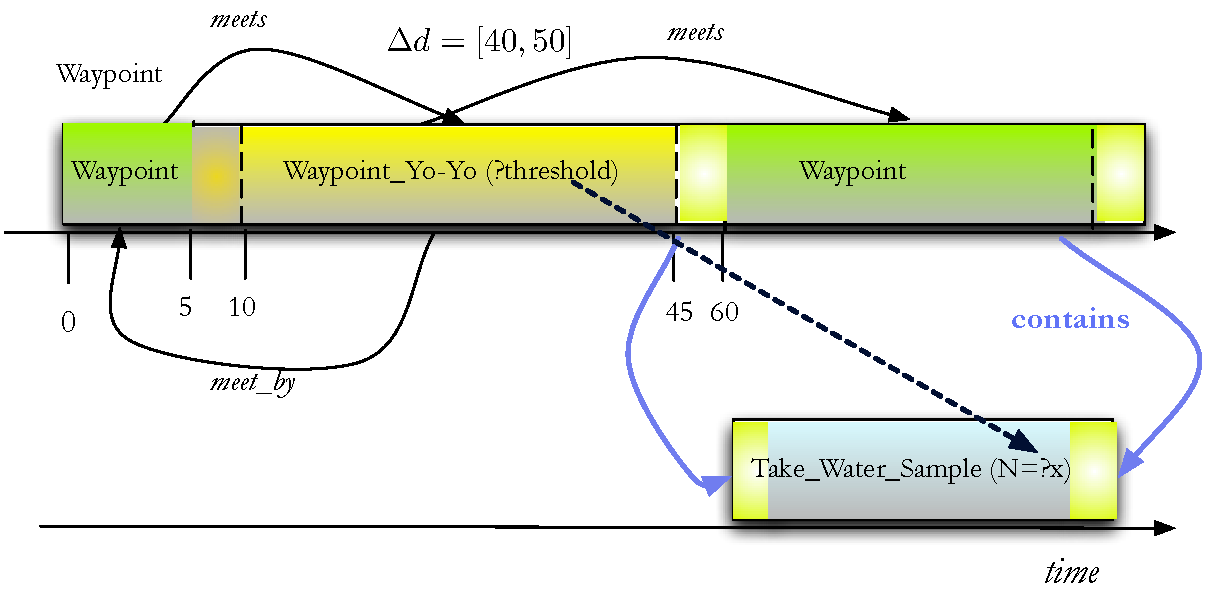
\includegraphics[scale=0.35]{figs/flexible-timelines.pdf}
\caption{\small Tokens with flexible temporal intervals and parametric
  constraints between tokens. This example shows the triggering of a
  water sampler based on a feature threshold while the vehicle
  Yo-Yo's. The \texttt{Waypoint\_Yo-Yo} token has a flexible duration,
  start \& end times.}
\label{fig:flex-timelines}
\vskip+0.1cm
\end{figure}

Unlike a traditional fixed time-tagged command sequences, such
flexible plans leave room for adaptation at execution time. When the
executive considers when to start a task, it propagates information
through the constraint network, computes a time bound for the
variable, selects an actual execution time within the bound, and
starts the task at that time. Temporally flexible plans therefore,
express a \textit{range of possible outcomes} of the robots
interaction with the environment within which the executive can elect
at run time the most appropriate one for the actual execution
conditions. The fact that constraints are explicitly represented
ensures that through constraint propagation the executive will respect
global limits expressed in the plan (e.g., don't start a task until a
certain condition has been satisfied but still satisfying some global
deadline). Such flexibility is critical when dealing with dynamic
ocean conditions where precise timing of a robotic action might be
indeterminate. Further, the advantage of flexibility can be contrasted
with the consequences of the intrinsic inflexibiliy of traditional
command sequences. Because they are inflexible, sequences must
necessarily be designed considering worst case scenarios.

\eu uses a \emph{state variable} representation to describe the
evolution of state over time. The instantiated history of such state
variable evolution over a temporal horizon we call \emph{timelines}
and which represent a single thread in the execution of a concurrent
system. At any given time each thread can execute a single procedure.
Thus each timeline consists of a sequence of procedures which
encapsulate and describe state evolution; we call these instantiated
atomic entities \emph{tokens}.  A token therefore describes a
procedure invocation, the state variables on which it can occur, the
parameter values of the procedure, and the time values defining the
interval. We allow encapsulation of uncertainty within these tokens
with a range of start and end times and parameters, all of which are
encoded as variables. A constraint solver in turn manipulates these
variables defined in a \eu domain model. For example, consider
a scientific need to take a water samples 100 meters from a hotspot
while an AUV is performing a Yo-Yo in the water-column. Two samples
are needed if the feature's signal is above a threshold; one
otherwise. The token that is capturing the sensory threshold has a
parametric constraints to the token which fires the requisite water
sampler. In addition, the start time of the water sampling procedure
is highly dependant on the variability of sub-sea currents and actual
speed of the vehicle. Therefore a number of values are possible for
the start times and duration of the sampling all of which are valid
combinations for desired outcomes.

\subsection{\eu Plan Representation}
\label{sec:europa:pr}

\eu follows the representation outlined by the CAIP framework, it also
adds a few elements to it that are necessary for an efficient
implementation of constraint-based planning. Below is a brief summary
of the main elements, followed by a detailed description for each one:


\begin{enumerate}

\item \textbf{Tokens} Temporally scoped entities that correspond to
  Intervals in the CAIP framework, are used to represent state and
  actions in time. A\textbf{Token State model} is defined to support
  an efficient implementation of plan-space search algorithms.

\item \textbf{Domains, Variables and Constraint} are used to represent
  restrictions in the problem domain in terms of a CP formulation.

\item \textbf{Domain Rules} are used to describe internal and external
  relationships on and between tokens, as presecribed by the CAIP
  framework.
  
\item \textbf{Objects} are used to represent problem domains in a more
  modular and scaleable way. \textbf{Timelines and Resources} are
  built in implementations of Object types that appear frequently in
  real life domains.

\end{enumerate}

\begin{description}

\item[\textbf{Variables}] Values that need to be represented to
  describe the problem domain and over which we may want to specify
  constraints. In the Shopping Agent example, the times at which the
  agent needs to leave or be back, or executes a purchase, are all
  instances where variables representing time would be used.  As
  explained in the \textsf{CP} section, a variable can take values
  from a domain. In \eu, domains are defined over a specific data
  type, the primitive data types supported are:

  \begin{enumerate}

  \item \textit{String}: sequences of characters, like "Red",
    "Spirit", etc

  \item \textit{Boolean}: {True,False}

  \item \textit{Numeric}: integers and floats

  \item \textit{Object}: reference to an object instance (see below
    for a description of objects in \eu)
  
\end {enumerate}

Two types of variable Domains can be defined over a data type:

  \begin{enumerate}

  \item \textit{Enumerated}: Finite sets over any data type, specified
    explicitly, for instance: ["Red","Yellow","Green"], [1,18,32], etc

  \item \textit{Interval}: Only for Numeric data types, they are
    specified by a [LowerBound,UpperBound] pair, for instance: [1,10],
    [5.0,100.0], etc.

  \end {enumerate}

  \eus ability to represent and reason over numeric intervals is a
  very useful characteristic that allow users to create flexible
  plans.

\item[\textbf{Constraints}] valid plans in most problem domains have
  to satisfy a number of restrictions, for instance, a Shopping Agent
  may only be able to perform one task at a time, may have limited
  time or an energy or fuel budget to perform a task, and so on. In
  \eu, these restrictions are represented by Constraints, which can be
  defined over any combination of Variables in a domain. \eu provides
  a Constraint Library that already implements many useful constraints
  (temporal, resource, relational, etc), it is also possible to add
  new constraints if required by a particular domain.

\item[\textbf{Objects}] The items we wish to describe and refer to in
  a domain are considered Objects. As in the case with object-oriented
  analysis and design, one can seek out the nouns in any domain
  description to find likely objects. In the Shopping Agent example,
  we might consider the Agent itself, Products and Locations all to be
  objects. Objects have state and behavior. For example, a Shopping
  Agent can have:

  \begin{itemize}

  \item State: its location, a bag that contains the products it has
    already purchased (the bag can in turn be another object), etc.

  \item Behavior: go to a location to look for a product, perform a
    purchase, return home, etc.

  \end{itemize}

  Objects that have similar state and behavior can be described
  generically in terms of object types or classes. \eu allows the
  definition of classes in the same way that it is done in popular
  object-oriented programming languages, where a class can have
  attributes (represented by Variables), and classes can be arranged
  in a single-parent hierarchy through inheritance.  However, one key
  aspect needs to be introduced to class definition in \eu that is not
  found in object-oriented programming: to describe state and behavior
  for the purposes of planning we need to build on the formalism of
  first order logic as explained below.

\item[\textbf{Tokens}] In first order logic, a predicate defines a
  relation between objects and properties \cite{gen87}.  In \eu, we
  define such relations between variables whose domains are sets of
  objects and sets of properties to describe state and behavior. For
  example, we might use a predicate \texttt{At($a$,$l$)} to indicate
  that agent $a$ is at location $l$, or a predicate
  \texttt{Buy($a$,$p$}) to indicate that agent $a$ is taking acting to
  buy product $p$. Note that $a$ is a variable which may have a number
  of possible values in a problem with multiple agents. Similarly, $l$
  and $p$ are variables whose values are the set of possible positions
  and products respectively. \eu can be used to create partial plans,
  where the domains of variables $a$ and $l$ can have more than one
  possible value in them, or grounded plans, where single values will
  be specified for each variable as we saw in the case of the
  N-queen's problem.

  In general, to come up with an executable plan it is not sufficient
  to state predicates that describe required state or behavior without
  also specifying some temporal extent over which each of those
  predicates hold. Predicates that are always true can be thought to
  hold from the beginning to the end of time. However, in practice,
  the temporal extent of interest must be defined with timepoints to
  represent its start and end. So we might want to write
  \texttt{At($a$,$s$,$e$,$l$)} to indicate that the agent $a$ is at
  location $p$ from time $s$ to time $e$. In fact, this pattern of
  using such predicates to describe both state and behavior of objects
  is so prevalent in \eu that we have introduced a special construct
  called a Token which has the built in variables to indicate the
  object to which the statement principally applies and the timepoints
  over which it holds. A Token is an instance of a predicate that
  represents and object's state or behavior and is defined over a
  temporal extent. In \eu, all predicate instances are Tokens. Also,
  in the same way that objects are described generically by classes,
  in \eu Tokens can be described generically by Token Types. Every
  token has five built-in variables:

  \begin{enumerate}

  \item \textit {start}: The beginning of the temporal extent over
    which the predicate is defined.

  \item \textit {end}: The end of the temporal extent over which the
    predicate is defined.

  \item \textit {duration}: The duration of the temporal extent over
    which the predicate is defined. The constraint \textit{start} $+$
    \textit{duration} = \textit{end} is enforced automatically.

  \item \textit{object}: The set of objects to which a token might
    apply. In a grounded plan each Token applies to a specific Object,
    reflecting the intuition that we are using Tokens to describe some
    aspect of an Object (i.e. its state or behavior) in time. However,
    in a partial plan, the commitment to a specific object may not yet
    have been made.

  \item \textit{state}: Tokens can be \texttt{ACTIVE, INACTIVE,
      MERGED}, or \texttt{REJECTED}. The state variable captures the
    token's current state and its reachable states through further
    restriction.  This is required to support CAIP's approach to
    planning where goals and subgoals can be satisfied by either
    adding new intervals (Tokens) to the plan, or by merging with
    existing intervals. Token State lifecycle is examined in detailed
    in a separate section below.

  \end{enumerate}

\item[\textbf{Built-in Object Types}] In a domain model, there may be
  some classes that don't have any time-dependent state or behavior,
  and therefore those classes will not have any Token types associated
  with them, for instance in the Shopping Agent model, the set
  locations and products are static for the agent's purposes so we may
  only want to say what they are but not have any state or behavior
  associated with them.

  However, the most common case in any non-trivial domain model is
  that Objects will have many associated Tokens in order to describe
  their state and behavior throughout a plan. There are a couple of
  Object Types that are so commonly used in domain descriptions, that
  \eu provides a built-in implementation for them:

\begin{enumerate}

\item \textit{Timelines}: Often objects in a domain must be described
  by exactly one token for every given timepoint in the plan. Any
  instances of a class derived from \eus built-in Timeline class will
  induce ordering requirements among its tokens to ensure no temporal
  overlap may occur among them \cite{mus94}.  \comment{Maybe: add
    small example?}

\item \textit{Resources}: Metric resources, e.g. the energy of a
  battery or the capacity of a cargo hold, are objects with an
  explicit quantitative state in time and with a circumscribed range
  of changes that can occur to impact that state i.e. produce,
  consume, use, change.  Resources are such a common requirement for
  \eu users that built-in object types (with their corresponding token
  types to denote production, consumption, etc) are provided for
  them. Instances of classes derived from a Resource will induce
  ordering requirements on their Tokens in order to ensure that the
  level of the resource remains within specified limits.
  \comment{Maybe: add small example?}
\end{enumerate}

\item[\textbf{Token State Model}] In \eus representation, goals are
  temporally scoped states that need to be achieved, or actions that
  must be performed. As a result, \eu internally represents goals as
  Tokens.  Goals can be posted explicitly, for instance, when a user
  asks the Shopping Agent to own a specific product by a specific
  time, or implicitly when subgoals are created as a result of domain
  compatibilities (described in the CAIP framework above), for
  instance, when the Shopping Agent must get to a Location where a
  Product is available before it is able to purchase it, in this case
  the original goal of purchasing the product will spawn a subgoal of
  being at a specific location.

  Looking at a how a simple Shopping Agent goal would be addresed by
  \eu helps illustrate how Token States support the planning process.

  Let's assume we start with a partial plan that places the Shopping
  agent at home at time 0 and with no Products in its possession, then
  we post a goal for the Shopping Agent to own a Drill at time 10.

  \comment{Use Fig 4 and edit:: Add figure showing an AgentLocation
    timeline with an At(Home) token with start=0 and end open, an
    empty AgentBag timeline, and a Own(Drill) token with start=10
    floating below both timelines}

  Note that the \texttt{Own(Drill)} token that represents the goal is
  not immediately placed on the \texttt{AgentBag} timeline since \eu
  must determine whether it can achieve that goal and how. When the
  goal is posted and before any decisions are made on it, the
  \texttt{Own(Drill)} token is created in an INACTIVE state, then \eu
  looks at the current partial plan and considers 2 alternatives:

\begin{enumerate}

\item If there are any tokens in the plan that are compatible with the
  new goal, \eu may attempt to satisfy the goal by merging it with any
  of them (if there is more than one it can try them one at a time),
  in this case, the state of the token would change to
  \texttt{MERGED}.

\item Instead of merging with existing tokens in the plan, \eu may
  decide to insert the new token into the plan, in that case its state
  would change to ACTIVE.

\end{enumerate}

When a token is merged, all restrictions imposed on the merged token
are transferred to the active token upon which it is merged. Merging a
token requires finding a target active token that is compatible with
the inactive token. Two tokens are merge-compatible if they are
instances of the same predicate and that no intersections between
corresponding variables are empty. The effect of merging is
illustrated in Figure 3.

\comment{Use previous fig and modify as appropriately:: Add figure
  showing the effect of merging; all figs on this section are
  conjoined. JB to sketch it out.}

When a token is activated all compatibilities associated with its
token type are evaluated, which may lead to new subgoals being
generated. In our example, there should be a compatibility stating
that the Shopping Agent must be at the same location as the product it
is purchasing. In that case, activating the \texttt{Own(Drill)} token
will cause a new \texttt{At(Drill.location)} to be created in an
INACTIVE state, which in turn will have to be dealt with.

\comment{Use previous fig and modify as appropriately: Add figure
  showing the effect of activating the token by putting it on the
  AgentBag timeline, and a new At(Drill.location) token floating
  below}

If neither activating nor merging works, a token may become REJECTED,
this is possible only for goals posted by the end user and specified
as optional. Subgoals generated as a result of token activation cannot
be rejected, if a subgoal cannot be satisfied through activation or
merging then it will cause the original activation decision that
spawned it to be retracted (\eus search mechanisms are explained in
detail in a separate section later on).

As we can see, a token's state can go from \texttt{INACTIVE} to
\texttt{ACTIVE, MERGED} or \texttt{REJECTED}, this lifecycle is
illustrated in the figure below.

\comment{Maybe: Add figure showing possible state transitions. Need a FSM.}

\item[\textbf{Rules}] In order for a plan to be valid, it must comply
  with all rules and regulations pertinent to the application domain
  in question. Rules govern the internal and external relationships of
  a token. For example, consider a parameterized action
  \texttt{Go(origin,destination)} which describes a Shopping Agent
  traveling from one location ( \textit{origin}) to another (
  \textit{destination}). The parameters are instantiated on a token as
  variables whose domain of values is the set of all locations in a
  given problem. A rule governing an internal relationship among token
  variables might stipulate that a transition must involve a change in
  location. This can be easily expressed as a constraint on the
  definition of a predicate of the form: \textit{origin !=
    destination}. It makes sense to further stipulate that the agent
  must be located at \textit{origin} before travel can happen and the
  agent must be located at \textit{destination} when completed. This
  is an example of a rule governing an external relationship among
  tokens. It specifies a requirement that tokens of the predicate
  \texttt{At} that represent the location state for the Shopping Agent
  precede and succeed tokens of the predicate \texttt{Go} that
  represents traveling.

  \comment{Use previous fig and modify as appropriately (used as
    above): Add figure showing internal and external relationships
    from rules on action Go. Need a fig from JB}

  Figure xx illustrates the entities and relations involved in
  specifying such a rule on a \texttt{Go} action. The token on which
  the rule applies is referred to (\texttt{Go}) as the master. Each
  \texttt{At} token required by the master is referred to as a
  slave. All variables are indicated by name and their domains are
  expressed as intervals in the case of temporal variables and as
  enumerations for the remainder. Application of a rule on a token can
  thus cause slave tokens, variables, and constraints to be
  introduced.

  The capability of a domain rule to cause a slave token to be created
  is a key vehicle through which planning occurs. Semantically, this
  rule imposes a requirement for supporting (slave) tokens to be in
  the plan in order for the master to be valid.


\end{description}

%\begin{figure*}
%\centering 
%\subfloat[]{\label{fig:plan-evolve1}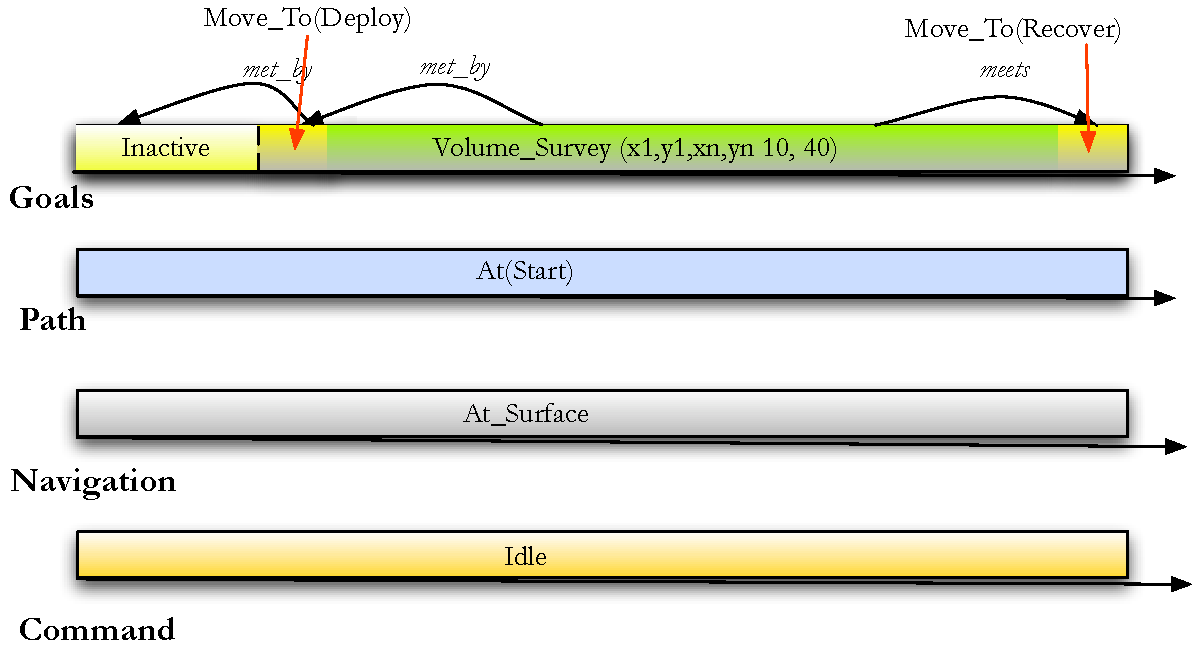
\includegraphics[width=0.3\textwidth]{figs/Plan-evolve-1.pdf}} 
%\subfloat[]{\label{fig:plan-evolve2}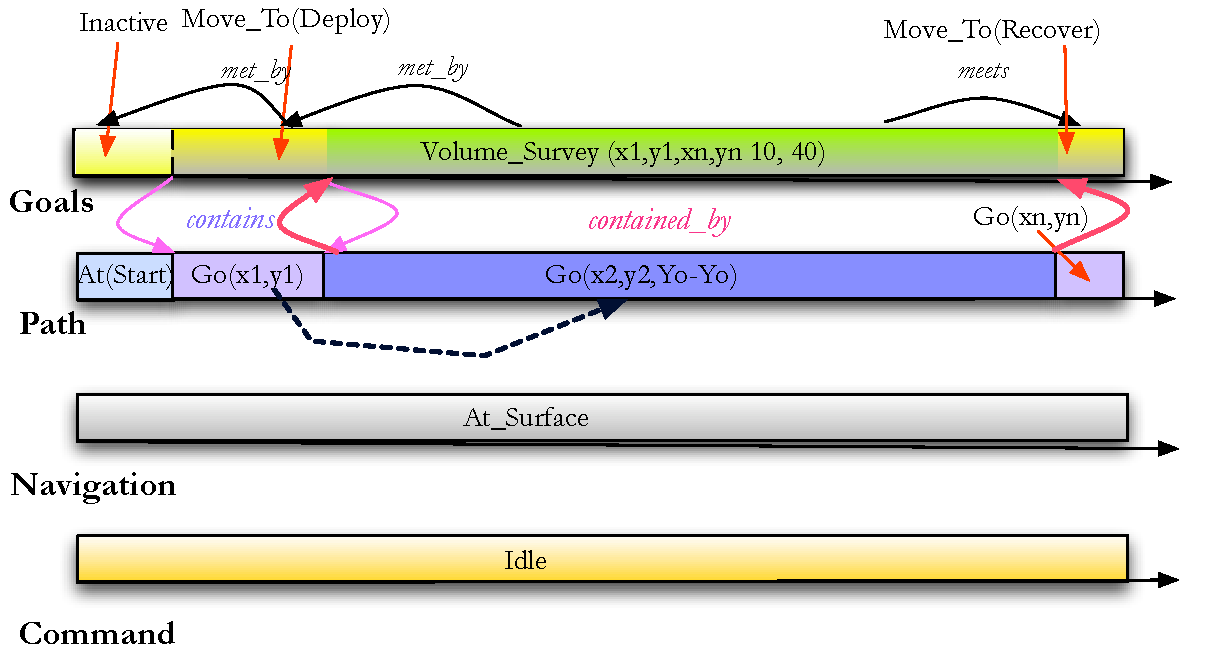
\includegraphics[width=0.3\textwidth]{figs/Plan-evolve-2.pdf}} 
%\subfloat[]{\label{fig:plan-evolve3}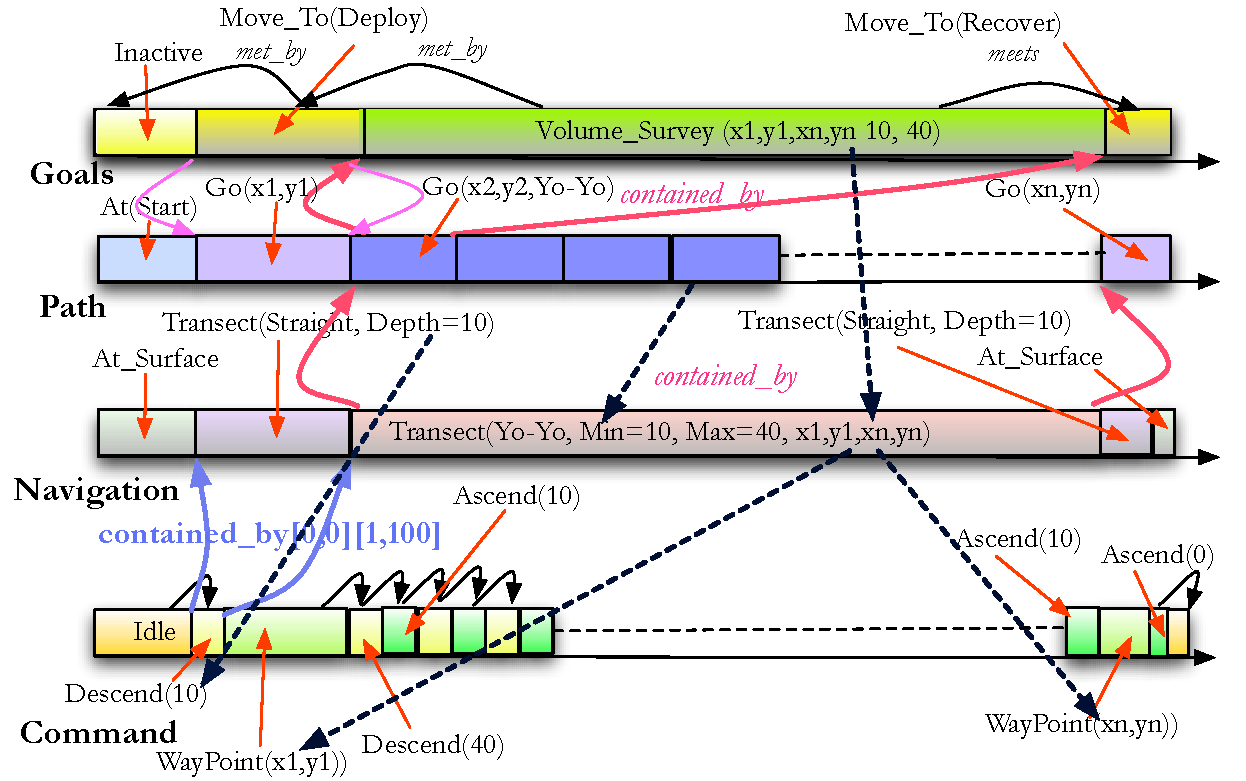
\includegraphics[width=0.3\textwidth]{figs/Plan-evolve-3.pdf}} 
%\caption{\small An illustrative plan synthesis example with concurrent
%  timelines. Each timeline is an instantiation of a subsystem tracked
%  by the planner. Tokens describe the instantiated state of subsystem
%  at a particular time instance and enforce temporal and parametric
%  constraints. Abstract goals are decomoposed into successively less
%  abstract tokens and instantiated in co-temporal timelines using
%  \texttt{Allen Algebra} relations. All tokens represent flexible
%  start/end times. \ref{fig:plan-evolve1} shows an initial state
%  evolving into \ref{fig:plan-evolve2} and \ref{fig:plan-evolve3}.}
%  \label{fig:Plan-evolve}
%  \vskip-5pt
%\end{figure*}

%Fig. \ref{fig:Plan-evolve} shows an illustrative example. We show four
%timelines which track \texttt{Goal, Path, Navigation} and
%\texttt{Command} state over time. Tokens on the goal timeline indicate
%a survey within a bounded volume and a min/max depth envelope. As the
%Volume Survey sub-goals on the \texttt{Path} timeline, the initial
%token on that timeline gets \emph{squeezed} to have dependencies of
%the goal token instantiated. Initially this dependency are the tokens
%\texttt{Go(x1,y1)} and \texttt{Go(xn,yn)} indicative of the area of
%coverage. The first of these in turn generates a sub-goal on the same
%timeline to go to the next intermediate waypoint, which is illustrated
%in Fig. \ref{fig:plan-evolve2}. Subsequent sub-goals (not shown in the
%figure) ultimately generate all the tokens to completion for this
%timeline. Fig. \ref {fig:plan-evolve3} shows a snapshot further along
%in plan generation and shows additional subgoals on the \texttt{Path,
%  Navigation} and \texttt{Command} timelines. Each token can thus
%trace its causality when instantiated in the plan. The domain model
%provides source of these temporal and parametric dependencies in the
%form of rules. 

%\begin{minipage}[c]{\textwidth}
%\vspace{+0.5cm}
% \framebox[\textwidth][t]{
%Volume\_Survey(x$_1$,y$_1$,x$_n$,y$_n$,Min\_Depth, Max\_Depth)\\
%$\Rightarrow$ \\
%met\_by Go(x$_1$,y$_1$,Min\_Depth); \\
%starts [50,0] Go(x$_2$,y$_2$,Min\_Depth,Max\_Depth); \\
%\ldots{} \\
%ends [50,0] Go(x$_{n-1}$,y$_{n-1}$, Min\_Depth,Max\_Depth); \\
%meets Go(x$_n$,y$_n$,Min\_Depth, Max\_Depth); 
%\end{minipage}

% \end{enumerate}



% \subsubsection{Partitioned Control}


% \subsubsection{State Estimation}

% Even as automated reasoning approaches have the ability to dynamically
% retarget the vehicle, estimating environmental signals of interest (or
% their proxies) is important to be able to enable opportunistic science
% in the water-column. In \texttt{T-REX} feature recognition revolves
% around a Hidden Markov Model (HMM) \cite{rabiner86} which is encoded
% directly within the unified representational and computational
% framework of a reactor. HMMs are useful since the stochastic nature of
% these models can correlate the type of features we want to detect with
% the sensor observations. Online targeted sensor data is classified by
% apriori generated cluster data which in turn determines the
% probability of having seen the feature of interest. Together with
% posterior probability, the HMM generates a probability of being within
% the target feature if it dominates the distribution. If other sampling
% conditions are satisfied (for instance sampling proximity), a
% constraint is activited in the model which can trigger a water sampler
% and also preserve the memory of sampling to alter a future transect
% resolution.


% The HMM is customized for the feature of interest and is built offline
% using clustering techniques from large data sets; we use Kohonen's
% Self Organizing Maps \cite{kohonen}. We use a semi-supervised learning
% method \cite{zhu05} to extract an environmental model that make uses
% of both labeled and unlabeled data for training. Online,

% The sensor data for classification depends on the
% feature of interest; for detecting INLs we use backscattering data
% from a HydroScat and for tracking riverine plumes to track fertilizer
% runoff, we use an ISUS Nitrate sensor.

%%% Local Variables: 
%%% mode: latex
%%% TeX-master: "ieee-ram09"
%%% End: 


\subsection{Architecture}
\label{sec:europa:arch}

\eu is implemented as a library that encapsulates all elements
described above making them accessible via modeling and Application
Programming Interface (API) layers.  A user will typically use the
modeling facilities to inject a problem domain description and the
API to extract and manipulate plans and to obtain information about
plan flaws and constraint violations at any stage of the planning
process.

\begin{figure}[b]
\centering
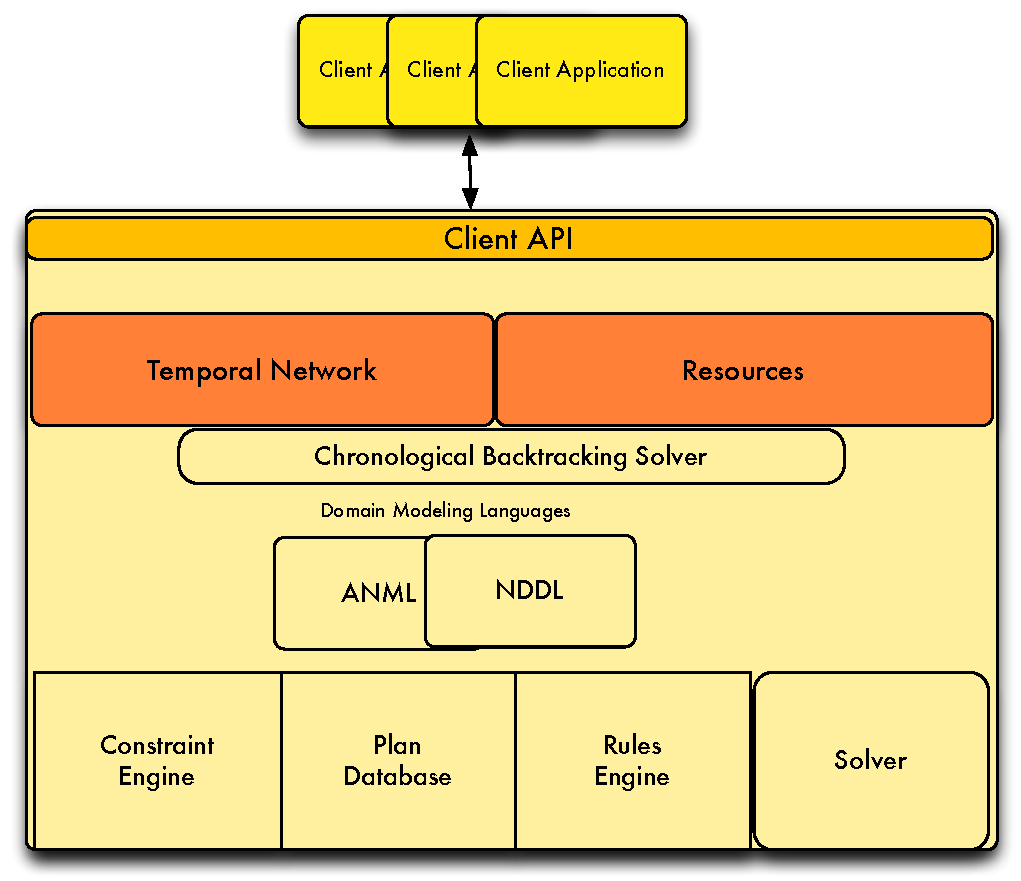
\includegraphics[scale=0.5]{figs/EUROPA-Architecture.pdf}
\caption{\small The \eu software architecture.}
\label{fig:europa-architecture}
\end{figure}

Fig. \ref{fig:europa-architecture} shows the main architectural
components in \eu and their relationships. The \textbf{Constraint
  Reasoning Engine} (\texttt{CRE}) manages domain types, variables and
constraints that define relationships among them. It also provides an
efficient arc consistency mechanism \cite{mackworth77}. The
\texttt{CRE} is designed so that specialized reasoning algorithms for
new constraints can be easily and efficiently plugged in. The
\textbf{Plan Database} (\texttt{PDB}) manages object and token
types. It also maintains the state of partial plans in terms of
object, variable and token instances. This constitutes the data
foundation on which end user applications and automated problem solvers
 are built. The \textbf{Rules Engine} (\texttt{RE})
modularly adds the semantics of domain rules that describe
dependencies between tokens. The \textbf{Solver Module} provides the
framework for flaw detection and resolution that is needed to
implement search algorithms for planning. The \textbf{API Layer}
provides access to services from all the different modules in a
programmatic way so that \eu can be easily embedded into specialized
applications.

Describing problem domains and problem instances in terms of objects,
variables and domain rules in a programmatic way is cumbersome to the
extent of being impractical; this motivated the creation of modeling
languages that support those definitions in a much more natural and
compact way. \texttt{NDDL} (New Domain Description Language
[pronounced ``noodle'']) \cite{NDDL} is the main modeling language for
\eu and will be described in detail in the Modeling section
below. Another, \texttt{ANML} is a language under development that
provides a more intuitive syntax \cite{smith08}.
  
In an effort to mimimize the amount of work that a user needs to
perform to solve specific problems, \eu also bundles extension
modules that have been found to be useful in many domains:

\begin{enumerate}

\item \textit{Temporal Network}: Extensions to the \texttt{CRE} module to
  reason about temporal constraints

\item \textit{Resources}: Extensions to the \texttt{CRE}, \texttt{PDB}
  and Solver modules to provide reasoning and search for metric
  resources.

\item \textit{Chronological Backtracking Solver}: A general purpose
  built-in solver to provide the ability to plan out-of-the-box.
  Problems that require challenging search may require specialized
  solvers to be built as explained in Section \ref{sec:europa:search}.

\end{enumerate}

\subsection{Modeling in \eu}
\label{sec:europa:modeling}

\eu can ingest descriptions of models, plans and goals and thereby can
be applied to different domains and problems, simply by providing
different models and goals. Consequently the expressiveness of the
language for models, goals and plans is of great importance. For \eue,
\texttt{NDDL} allows the user to specify the different components of a
problem domain in a precise and concise manner. Among the main
features that make \texttt{NDDL} a powerful tool for describing
problem domains are that it is object oriented. \texttt{NDDL} supports
classes and inheritance in similar fashion to popular Object-Oriented
languages like Java and C++. It also supports polymorphism for some of
the planning components. Using object classes and instances is a
time-tested approach to naturally describe problem domains
\cite{rumbaugh}. It offers declarative constructs to define
constraints and causality dependencies between actions and effects and
finally it offers procedural constructs to populate \eus \texttt{PDB}
with specific problem instances expressed in terms of objects,
variables, constraints, facts and goals. To articulate the most important
elements of \texttt{NDDL}, we show how the Shopping Agent problem
could be modeled:

\begin{verbatim}

// Locations (Home, SuperMarket, etc.)
class Location {
  string name;
  Location(string _name){
    name = _name;
  }
}

// Products (Milk, Banana, etc.) and
class Product {
  string name;
  Product(string _name) {
    name = _name;
  }
}

// ProductLocations (Banana can be found at SuperMarket, for example)
class ProductLocation {
  Location location;
  Product product;

  ProductLocation(Location _location, Product _product){
    location = _location;
    product = _product;
  }
}

// Use built-in Timeline functionality to enforce that an agent:
// a) Can't be at more than one place at a time.
// b) Can't Go more than one place at a time.
// c) Can't Go somewhere and be At somewhere at the same time.
class AgentLocation extends Timeline{
  predicate At {
    Location loc;
  }

  predicate Going {
    Location from;
    Location to;
  }
}

// In addition to having a location timeline, the agent can buy and own things.  
// Note that the actions and the location predicates can be concurrent 
// so they can't be on the same Timeline
class Agent {
  AgentLocation location;

  Agent() {
    location = new AgentLocation();
  }

  action Buy {
    Product product;
  }
  
  action Go {
    Location from;
    Location to;
  }
  
  predicate Own {
  	Product product;
  }
}
\end{verbatim}

In the model above one can see how the main elements of a problem domain
can be mapped to \eus representation:

\begin{description}

\item[\textbf{Object Types}:] \texttt{NDDL} supports an object-oriented
  approach, where common data and behavior can be abstracted as a
  class. In this case, we have the \textit{Product} class represent
  the products that the Shopping Agent needs, \textit{Location}
  represents the places where products can be found,
  \textit{ProductLocation} represents the association arising when a
  product can be purchased at a location. The Shopping Agent itself is
  represented by an \textit{Agent} class, which relies on the
  \textit{AgentLocation} class to keep track of where the agent is at
  any point in time. \texttt{NDDL} supports a single rooted class
  hierarchy so that state and behavior can be extended through
  inheritance. We take advantage of that feature by making
  \textit{AgentLocation} inherit from \eus built-in \textit{Timeline}
  class which doesn't allow predicates to overlap in time for the same
  object instance. This feature is used for instance, to ensure that
  an agent can only be at one place at a time in our example.

\item[\textbf{Variable Types and Instances}:] All object attributes
  are represented as variables in this model. For instance, it uses
  integer variables to represent the built-in temporal parameters for
  each token (duration, start and end times), string
  variables to represent \textit{Location} and \textit{Product} names,
  and object reference variables to represent the structural
  relationships between different objects (for instance, each Agent
  maintains a variable to keep track of its \textit{AgentLocation}).

\item[\textbf{Predicate Types}:] Some classes like \textit{Product},
  \textit{Location} and \textit{ProductLocation} are static and so
  don't have any predicate or action types associated with them. The
  \textit{AgentLocation} class is used to keep track of state and so
  has \texttt{At} and \texttt{Going} predicate types associated with
  it. The \textit{Agent} class keeps track of the products it
  purchases through the \texttt{Own} predicate; having a separate
  \textit{AgentBag} class with its own predicates would have been an
  equally valid modeling choice.

\item[\textbf{Action Types}:] In our example, \textit{Agent} is solely
  the class that has behavior associated with it. Consequently, it
  defines action types to represent when the agent is taking action to
  \texttt{Go} to a \textit{Location}, or to \texttt{Buy} a
  \textit{Product}. 
  
\end{description}

\begin{verbatim}

// Define the rules for our actions:
Agent::Go {
  met_by(condition object.location.At origin);
  eq(from, origin.loc);
 
  equals(effect object.location.Going going);
  eq(going.from, from);
  eq(going.to, to);
   
  meets(effect object.location.At destination);
  eq(to, destination.loc);
}

Agent::Buy {
  // A Buy takes 10 time units
  eq(10, duration);

  // initialized to all locations
  ProductLocation possibleStores;

  // limit possibleStores variables to ones that provide what we need to buy
  eq(product, possibleStores.product);

  // We must be At a location during our Buy, and that location must have the
  // product we want available:
  contained_by(condition object.location.At currLocation);
  eq(currLocation.loc, possibleStores.location);
  
  meets(effect Own purchase);
  eq(purchase.product,product);
}
\end{verbatim}

Domain rules can be defined in \texttt{NDDL} in the context of a
predicate or an action. In the example above we can see the main
elements of a rule definition:

\begin{description}

\item[\textbf{Variables}:] A token type (predicate or action) is part
  of a class, therefore class attributes (see \texttt{object.location}
  above), token type parameters (see \texttt{[from, to]} in
  \texttt{Agent::Go}, or \texttt{[duration, product]} in
  \texttt{Agent::Buy}) and locally declared variables (see
  \texttt{possibleStores} in \texttt{Agent::Buy}) can all be used in
  the definition of a rule.

\item[\textbf{Constraints}:] Restrictions on values that variables can
  take within a rule are expressed through constraints. In the example
  above the \texttt{eq} constraint is used; in general, any constraint
  available in \eus library can be used.

\item[\textbf{Subgoals}:] In \texttt{Agent::Go}, subgoals are used to
  specify that the Shopping Agent's location must transition from
  origin to destination in a temporally consistent way. The
  \texttt{[meets, equals, metby]} operators (see Section
  \ref{sec:europa:inference}) are used to specify subgoals, along with
  the temporal relationship each token representing a subgoal has with
  the the token representing the \texttt{Agent::Go} action. Also,
  \texttt{[condition, effect]} annotations can be used when defining a
  subgoal inside an action. \eu does not intrinsicaly associate semantics
  with these annotations; but they can be extremely useful for search
  modules when creating plans.

\end{description}

With that specification for the Shopping Agent domain, a particular
problem instance could be stated as follows:

\begin{verbatim}

// Allocate instances
Location Home = new Location("Home");
Location SuperMarket = new Location("SuperMarket");
Location HardwareStore = new Location("HardwareStore");

Product Banana = new Product("Banana");
Product Milk = new Product("Milk");
Product Drill = new Product("Drill");

ProductLocation bananaLocation = new ProductLocation(SuperMarket, Banana);
ProductLocation milkLocation = new ProductLocation(SuperMarket, Milk);
ProductLocation drillLocation = new ProductLocation(HardwareStore, Drill);

Agent agent = new Agent();

// Indicate that the database is closed - no new objects can be created
// this allows EUROPA to perform more efficient inference
close();

// We start the day at Home:
fact(agent.location.At atHomeForBreakfast);
atHomeForBreakfast.loc.specify(Home);

// Goals for all of the agent's needs, buy if needed
goal(agent.Own gotMilk);
gotMilk.product.specify(Milk);
goal(agent.Own gotBanana);
gotBanana.product.specify(Banana);
goal(agent.Own gotDrill);
gotDrill.product.specify(Drill);

// Make sure agent is home for dinner
goal(agent.location.At atHomeForDinner);
atHomeForDinner.loc.specify(Home);

// Agent has all day to satisfy goals:
gotMilk after atHomeForBreakfast;
gotMilk before atHomeForDinner;

gotBanana after atHomeForBreakfast;
gotBanana before atHomeForDinner;

gotDrill after atHomeForBreakfast;
gotDrill before atHomeForDinner;

// Force things to happen within our planning horizon:
int horizonStart = 0;
int horizonEnd = 100;
leq(horizonStart, atHomeForBreakfast.start);
leq(atHomeForDinner.end, horizonEnd);

\end{verbatim}

This problem instance consists of \textbf{Variables} and
\textbf{Objects}, \textbf{Facts}, \textbf{Goals} and
\textbf{Constraints}. In our example we define temporal variables that
are used to specify the planning horizon (\texttt{horizonStart} and
\texttt{horizonEnd}) and objects are used to specify locations,
products, product-location associations and the Shopping Agent that we
want to plan for. Facts are used to specify the current state of the
world, do not need any support and are represented as tokens in the
\texttt{PDB}. In this case we use facts to specify that the Shipping
Agent is initially at home. Goals are also represented as tokens in
the \texttt{PDB}. Different from facts, goals trigger inference in \eu
which determines whether flaws (unresolved subgoals, overloaded
resources, etc.) need to be resolved; if so, search modules can be
invoked to resolve those flaws as part of the deliberation
process. Finally, constraints are restrictions on and between facts
and goals. In the example above, we use temporal constraints to
specify when facts hold and when the goals should be accomplished. In
the model above, \texttt{before} and \texttt{after} are \texttt{Allen
  Algebra} \cite{allen84} operators, which \eu supports to specify
temporal relations between tokens (specifically between their start
and end timepoints). The algebra is particularly effective in dealing
with interval arithmetic; its elements are summarized in
Fig. \ref{fig:allen-algebra}

\begin{figure}[!t]
\centering
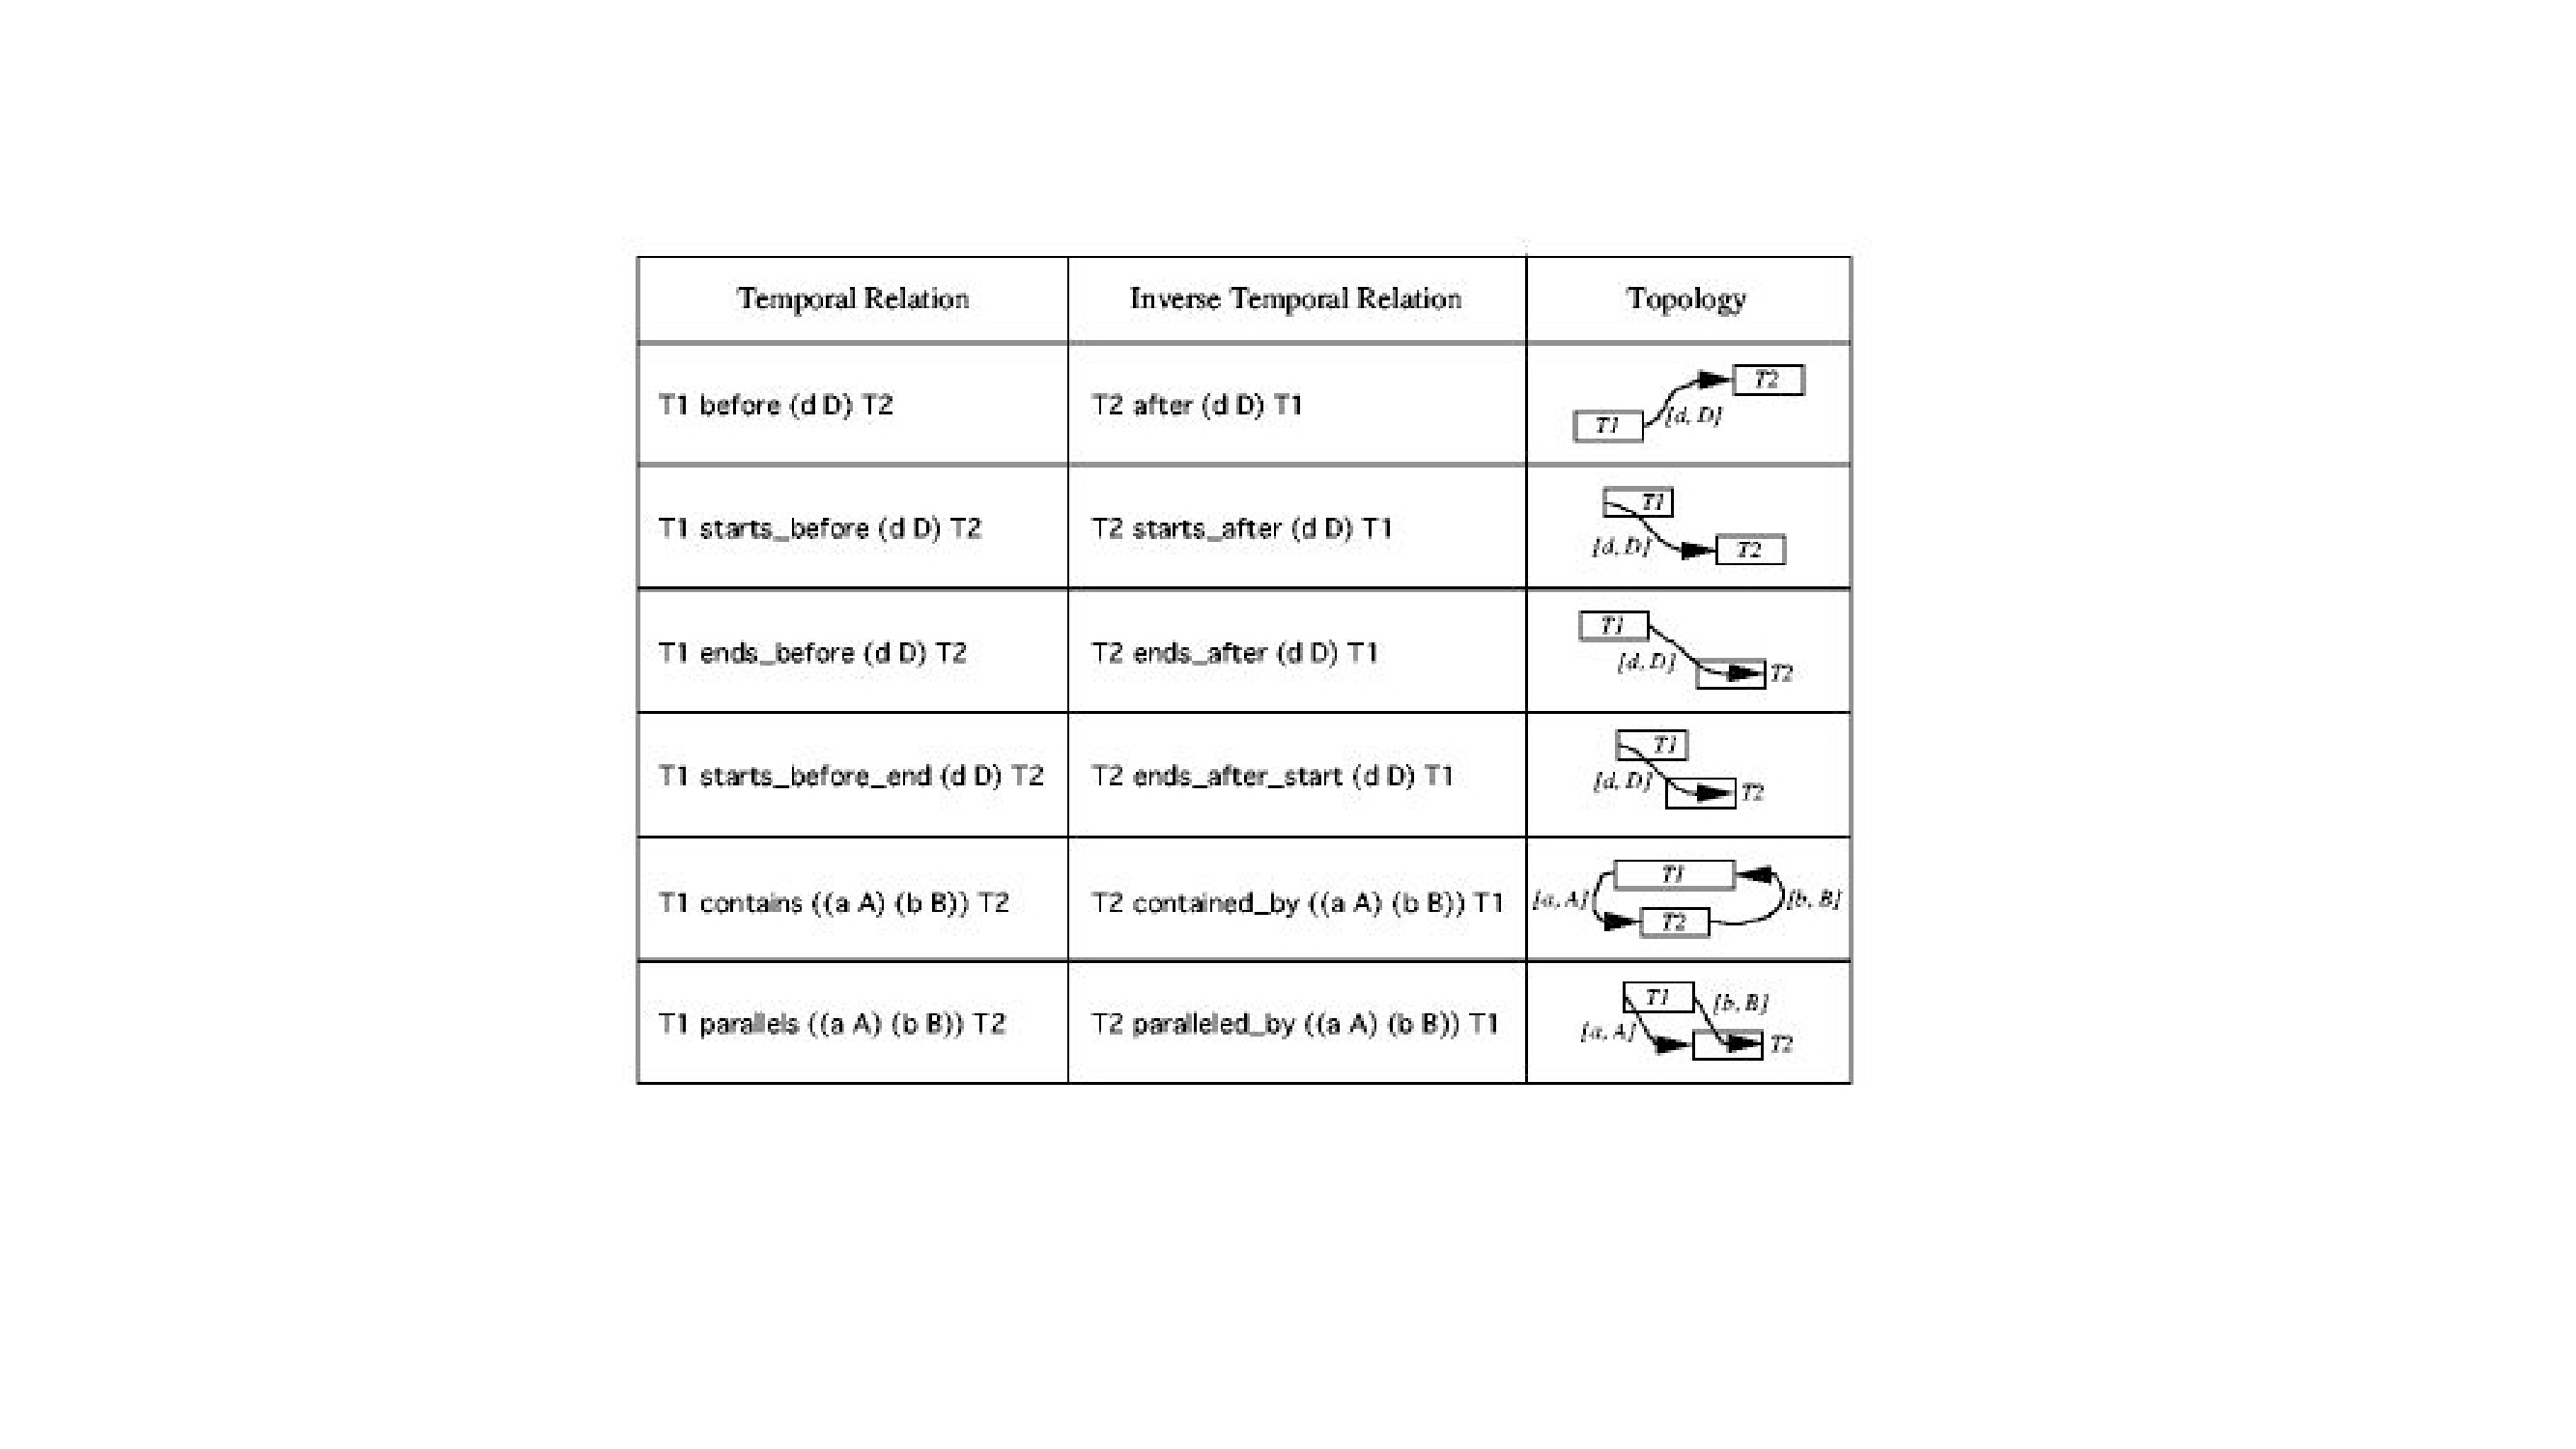
\includegraphics[scale=0.4]{figs/Allen-algebra.pdf}
\caption{\small Temporal relations defined within the planner are
  based on \texttt{Allen Algebra} \cite{allen84} relations shown
  above.}
\label{fig:allen-algebra}
\end{figure}


\subsection{Automated Inference}
\label{sec:europa:inference}

In \eue, all variables and constraints from a problem domain
description are stored inside the \texttt{CRE}.  The \texttt{CRE}
provides a framework where any number of constraint types can
collaborate to perform inference and prune variable domains using
Bounds Propagation and Domain Reduction techniques \cite{marriott98}. 
\eu uses a Propagator pattern which keeps track of a set of
constraint instances of the same type and is responsible for ensuring
variables are updated through inference whenever a relevant change occurs
 (variable domain modifications or constraint addition/deletion).

In a planning problem, variable or constraint changes can come
directly from an end user (by introducing new activities or goals and
relating them to the rest of the plan through constraints, by changing
the start or end time of an activity, etc), or from an automated planner (by
expanding subgoals, introducing precedence constraints to resolve
mutual exclusion conflicts, etc). When these changes occur, each
propagator is only able to ensure consistency for the constraints that
are associated with it.  To maintain global consistency, the
\texttt{CRE} implements a variant of the \texttt{AC-3} algorithm
\cite{mackworth77} where propagators are invoked repeatedly until
the constraint network returns to a quiescent state.

\subsubsection{Constraint Formulation}
\label{sec:europa:constraints}

An \eu user can introduce new constraint types by implementing
specialized constraint and propagator classes; however, \eu provides a
built-in constraint library with a range of arithmetic, temporal, set
and resource constraint types so that a large number of problem
domains can be modeled without having to introduce new constraint
types. Tables \ref{tab:calconst}, \ref{tab:setconst},
\ref{tab:objhierarchy} and \ref{tab:misc} show the main constraint
types included in \eus Constraint Library.

\begin{table*}[ht]
  \centering
  \renewcommand{\arraystretch}{1.0}%{0.99}
  \begin{tabular}{|l|l|p{7cm}|p{3cm}|}
    \hline
    \textbf{Constraint}& \textbf{Syntax}& \textbf{Description}& \textbf{Variable Types}\\
    \hline
    distanceSquares& distanceSquares(a,b,c)& c = sqrt(a+b) if a and b are singleton& Numeric intervals\\
    \hline
    calcDistance&calcDistance(a,b,c,d,e)& a is Euclidean distance between points (b,c) and (d,e)& Numeric intervals\\
    \hline
    sin& sin(a,b)& a = sin(b)& Numeric intervals\\
    \hline
    allDiff& allDiff(a,b,\ldots)& Restrict all domains so the intersection of any pair of domains is empty& Comparable\\
    \hline
    EqualMaximum& EqualMax(a,b,\ldots)& a = max(b,\ldots)& Numeric\\
    \hline
    EqualMinimum& EqualMin(a,b,\ldots)& a = min(b,\ldots)& Numeric\\
    \hline
    CountZeros& CountZeros(a,b,\ldots)& a is the count of the rest that can be zero& Numeric\\
    \hline
    CountNonZeros& CountNonZeros(a,b,\ldots)& a is the count of the rest that can be non-zero& Numeric\\
    \hline
    diffSquare& diffSquare(a,b,\ldots)& c = (a - b)$^2$ if a and b are singleton& Numeric intervals\\
    \hline
    card& card(a,b,\ldots)& a must be greater than or equal the count of the other variables that are true& Numeric\\
    \hline
  \end{tabular}
  \caption{\small Calculation Constraints: These constraints enforce that one variable (usually $a$) is constrained by a calculation done on the remaining variables.}
  \label{tab:calconst}
\end{table*}

%%%%%%%%%%%%%

\begin{table*}[ht]
  \centering
  \renewcommand{\arraystretch}{1.0}%{0.99}
  \begin{tabular}{|l|l|p{7.5cm}|p{3cm}|}
    \hline
    \textbf{Constraint}& \textbf{Syntax}& \textbf{Description}& \textbf{Variable Types}\\
    \hline
    subsetOf& subsetOf(a,b)& a is a subset of b& Comparable\\
    \hline
    memberImply& memberImply(a,b,c,d)& If a is a subset of b, then require that c is a subset of d& a and b comparable, c and d comparable\\
    \hline
    Lock& Lock(a,b)& Restrict a's domain to be contained in b's domain& Comparable\\
    \hline
  \end{tabular}
  \caption{\small Set Constraints: These constraints are likely to be used for set comparisons etc. Note, however, that many of the other constraints could be used for sets (\ie Comparable variables) just as these constraints could be applied to numeric domains as well.}
  \label{tab:setconst}
\end{table*}

%%%%%%%%%%%%%

\begin{table*}[ht]
  \centering
  \renewcommand{\arraystretch}{1.0}%{0.99}
  \begin{tabular}{|l|l|p{7cm}|p{3cm}|}
    \hline
    \textbf{Constraint}& \textbf{Syntax}& \textbf{Description}& \textbf{Variable Types}\\
    \hline
    commonAncestor& commonAncestor(a,b,c)& a and b must be contained by the same object in c (or by c itself)& a, b and c are all objects\\
    \hline
    hasAncestor& hasAncestor(a,b)& a must be contained by some object in b& a and b are objects\\
    \hline
  \end{tabular}
  \caption{\small Object Hierarchy Constraints: These constraints are imposed on objects and tokens. These constraints are used to assert which object one or more tokens is contained by. Most often, the commonAncestor constraint is used to subgoal across timelines which must share a contained object in common.}
  \label{tab:objhierarchy}
\end{table*}

%%%%%%%%%%%%%

\begin{table*}[ht]
  \centering
  \renewcommand{\arraystretch}{1.0}%{0.99}
  \begin{tabular}{|l|l|p{9.5cm}|p{3cm}|}
    \hline
    \textbf{Constraint}& \textbf{Syntax}& \textbf{Description}& \textbf{Variable Types}\\
    \hline
    UNARY& NA& Restrict a variable's domain; given a variable and a domain, intersect them. Note that this constraints is only available internally and not exposed in NDDL& Anything\\
    \hline
    or& or(a,b\ldots)& At least one of the variables must be true& Numeric\\
    \hline
    absVal& absVal(a,b)& a.lb $\geq$ 0, a.ub = max(abs(b.lb)), b.lb $\geq$ -a.lb, b.ub $\leq$ a.ub& Numeric\\
    \hline
  \end{tabular}
 \caption{\small Miscellaneous Constraints}
  \label{tab:misc}
\end{table*}



Temporal and resource constraints are especially important to model
real-world planning domains. 

\eu uses variables to explicitly represent timepoints for plan
actions and states. Constraints among timepoints provide a natural
way to express domain axioms. For example, in order to state that
activity $A$ must occur before activity $B$ we can say that the end
timepoint of $A$ is $leq$ the start timepoint of $B$.
\cite{dechter91} proposed that constraints among timepoints can be
grouped together to form a Simple Temporal Network
(\texttt{STN}). Such a network can be transformed into a Distance
Graph (\texttt{DG}) where the outward arc from a node represents the
maximum distance from the source node to the target node.
Fig. \ref{fig:stn} illustrates an \texttt{STN} with $2$ variables and
a single constraint along with the resulting \texttt{DG}.
\cite{dechter91} also showed that shortest path algorithms could be
used to propagate values in the network and discover a negative cycle:
namely a path from a node to itself that has a path length less than
$0$. If such a cycle exists, the network is inconsistent. It was
further shown that a single-source shortest path algorithm was
sufficient to detect a negative cycle and provide sufficient
propagation to yield a backtrack-free search. \eus propagator for
temporal constraints is a straight implementation of this algorithm.

\begin{figure}[!htb]
  \centering
  \subfloat[\small A Simple Temporal Network (STN)]{\label{fig:stn1}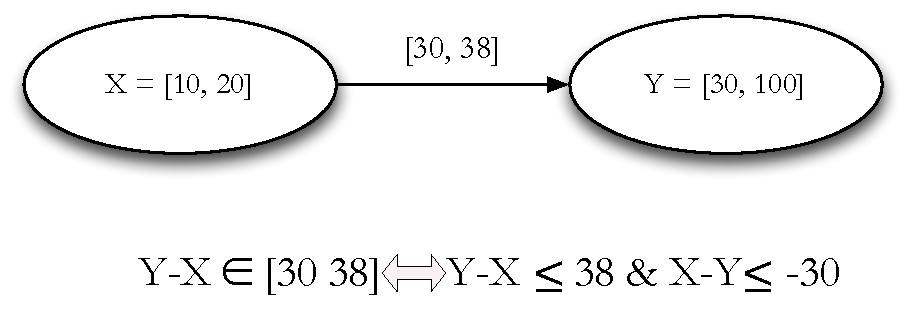
\includegraphics[width=0.4\columnwidth]{figs/stn-graph.pdf}}
  \subfloat[\small Resulting distance graph from \ref{fig:stn1}.]{\label{fig:stn2}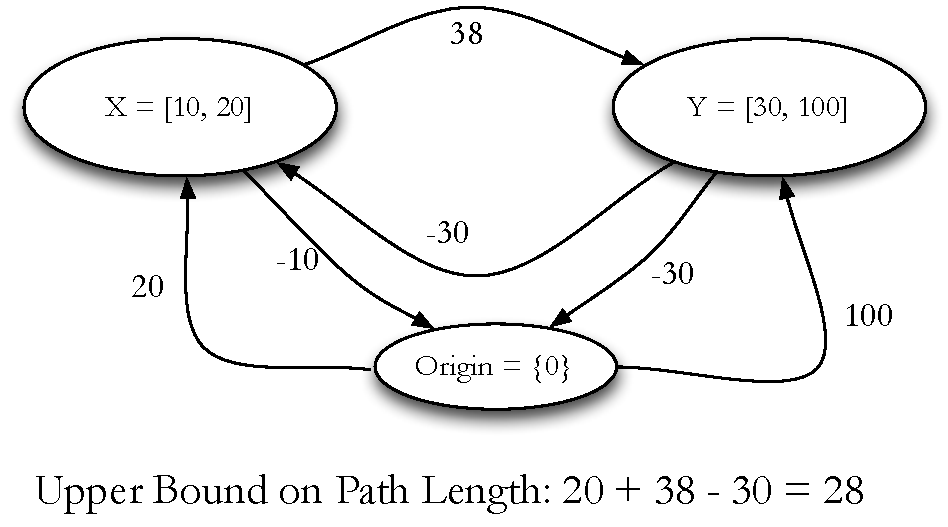
\includegraphics[width=0.4\columnwidth]{figs/distance-graph.pdf}}
  \caption{\small An illustration of a STN and its corresponding
    distance graph.}
  \label{fig:stn}
\end{figure}

Most real-world planning problems need to deal with plans made up of
actions that typically depend upon limited resources (\eg fuel,
storage capacity, battery state of charge, data buffers).  \eu
provides built-in support for resource computation. In \eus
representation resource object types come in three forms with related
constraints. \textbf{Reservoir} resources can have both
\texttt{consume(resource,time,quantity)} and
\texttt{produce(resource,time,quantity)} constraints; production and
consumption is instantaneous. \textbf{Reusable} resources on the other
hand, have constraints that use a quantity of the resource for a
specific duration (\texttt{uses(resource,start,duration,quantity)}),
which are then subsequently released. \textbf {Unary} resources are
reusables with capacity$ = 1$, which allows \eu to perform run time
savings in comparison to the generic reusable class. Configuration
options are offered such that in addition to the usual constraint
violations when a resource is completely depleted, plan flaws can be
generated whenever a resource level is outside a specific upper or
lower bound, or when instantaneous production or consumption exceeds a
specific threshold.

Since \eu supports a flexible temporal representation, where time is
represented by intervals, instead of single values, determining
whether a resource is the source of a plan flaw or a constraint
violation in general is substantially more difficult than just
computing a profile of the resource and checking against some limits.
With temporal flexibility, a number of resource profiles could be
possible depending on precisely when each production/consumption event
occurs out of a range of possible values that are in the domain of the
variables that represent the temporal extent for the event.
\cite{Muscettola04,Muscettola06} proposed an algorithm where the
variables that represent the time for production/consumption events
are placed in a temporal network, similar to the network used by the
temporal propagator; constraints on the resource can then be seen as
quantities flowing through that network. Computing the maximum flow
then, yields the maximum resource usage and thus a lower bound on the
resource level; computing a minimum flow will similarly yield an upper
bound. Since maximum flow on a temporal network can be computed in
polynomial time, \eu takes advantage of this algorithm to efficiently
compute upper and lower bound envelopes on the resource
level. Fig. \ref{fig:resenvelopes} shows an example of such a resource
computation.

\begin{figure}
\centering
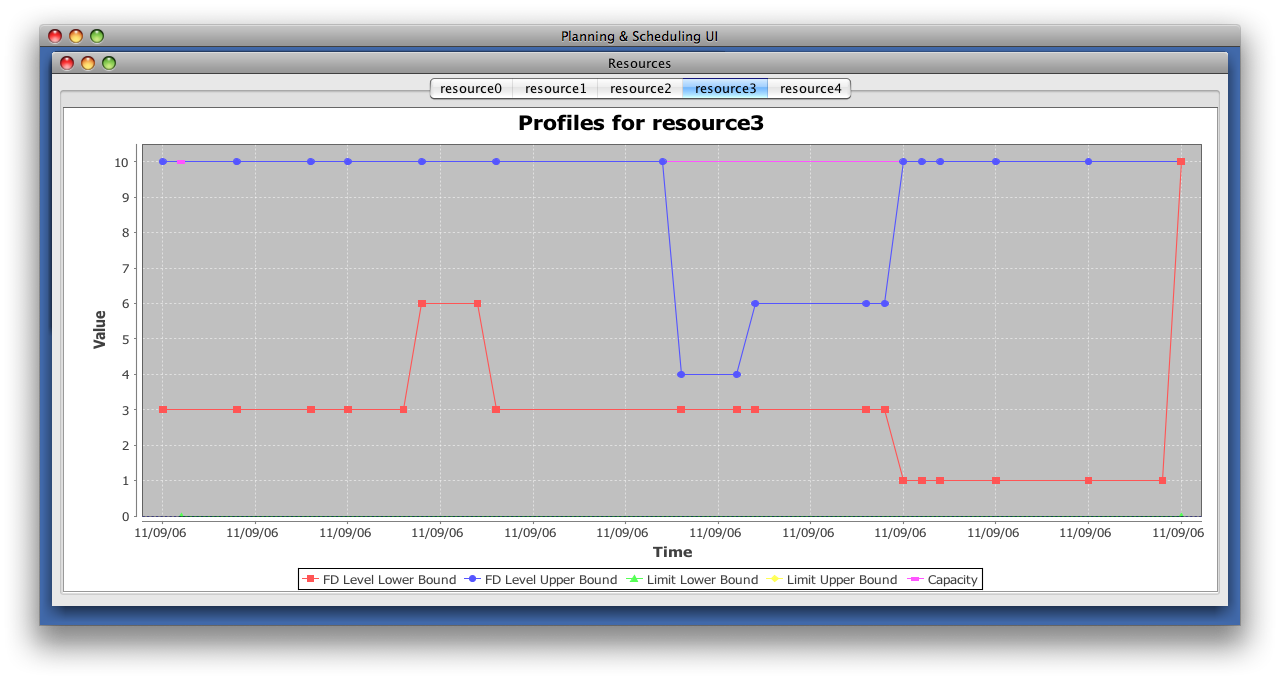
\includegraphics[scale=0.3]{figs/europa-resource-envelopes.png}
\caption{\small An example of resource envelopes computed by \eu.}
\label{fig:resenvelopes}
\end{figure}

Resource envelopes can be useful when trying to evaluate plan
brittleness in the face of changing activity durations or start
times. They can also be useful when searching for plans; however they
are relatively expensive to compute. Therefore their ability to prune
the search space must be weighted against the ability to search faster
\cite{6007772, morris11}.


\subsection{Search in \eu}
\label{sec:europa:search}

Given the above, an automated problem solver can be created using a
\emph{domain model} that describes the variable, object, predicate and
action types that are relevant for the problem, a \emph{problem
  instance} or initial state that consists of variable and object
instances that exist for the entire planning horizon, \emph{temporally
  scoped predicate and action} instances and \emph{temporally scoped
  goals}. This information is retained in \eus \texttt{PDB} so that
inference and search mechanisms can be used to look for a problem
solution.

Since temporal intervals may extend indefinitely in both positive and
negative directions, for problems with a temporal dimension it is also
common to specify a \emph{planning horizon} when invoking a solver;
any decisions that fall completely outside of the horizon can be
ignored. This is useful to ignore activities that may occur far in the
future or in the past to be relevant for a particular plan, ensuring
that the solver is making as few commitments as necessary and reducing
the complexity of plan generation.  The \emph{planning horizon} is
also useful when dealing with recurrent activities; consider for
instance a model where a medical checkup has to occur every $3$
months. The user can model a recurring activity and then use the
horizon to ensure that a finite number of medical checkup activities
are generated as part of a plan.

\subsubsection{Flaw Resolution}
\label{sec:europa:flaws}

\eu provides a built-in solver that performs \emph{Plan Space
  Planning} \cite{ghallab04}; the initial state is considered a
partial plan that needs to be refined toward a solution that achieves
stated goals. The operations to refine the partial plan \texttt{PP} at
any time are:

\begin{enumerate}

\item Find flaws of \texttt{PP}, \ie conditions that prevent it from
  being a solution plan.

\item Select one such flaw.

\item Select a resolver for the flaw.

\item Refine \texttt{PP} by applying the resolver.

\item If an inconsistency is found, try another resolver.

\item If all possible resolvers for a particular flaw fail, return
  failure, otherwise continue until resolving all flaws.

\end{enumerate}
	
The initial partial plan is the state of \eus Plan Database after the
initial state has been instantiated. This results in a set of
variable, object and token instances. Inference then takes place to
detect flaws in the partial plan; the three kinds of flaws that can be
detected are:

\begin{description}

\item[\textbf{Unbound Variable}:] a variable in the partial plan whose
  domain is not a singleton. Unbound Variables are resolved by value
  selection from their domain.

\item[\textbf{Open Condition}:] an open condition is an
  \texttt{INACTIVE} token. \texttt{INACTIVE} tokens can be generated
  by explicitly posted goals, or when a token is activated, rules may
  cause the creation of \texttt{INACTIVE} slave tokens as described
  in Section \ref{sec:europa:pr}. Open Conditions can be resolved in
  three ways:

  \begin{description}

  \item[\textbf{Merging}:] An \texttt{INACTIVE} token is merged with a
    matching \texttt{ACTIVE} token already in the plan. A token $a$ is said to
    match another token $a?$ iff $a$ and $a?$ unify \cite{russelnorvig}
    and the temporal constraints involving $a$ are satisfied by
    $a?$. Thus, $a$ and $a?$ can be considered the same token
    without the need to introduce $a$ in the plan. Consequently, the
    domain rules associated with $a$ are not introduced into the
    planning process, since they are already triggered when $a?$ was
    introduced in the plan.

  \item[\textbf{Activation}:] A token $a$ is introduced in the
    current plan associating it with the appropriate timeline, without
    choosing a specific time slot; if its timing causes a problem a
    Threat flaw will be triggered (see below).  The domain rules
    associated with $a$ are applied and the subgoal activities
    resulting from those domain rules are introduced as \texttt{INACTIVE}
    tokens.  This results in a number of open condition flaws,
    corresponding to the new subgoal activities.

  \item[\textbf{Rejection}:] Some goals may be optional; if so its
    corresponding flaw may be resolved by discarding the
    \texttt{INACTIVE} token.

  \end{description}

\item[\textbf{Threat}:] Once a token has been placed in the partial
  plan it may impact other tokens indirectly through possible
  overlapping requirements on objects. Recall for example that a token
  may belong to objects (\eg timelines) which require a total order
  over their tokens. If any two tokens could possibly overlap (though
  not necessarily), then they pose a threat to each other in terms of
  achieving an extension of the current partial plan which is complete
  and consistent. Similarly, threats may arise where tokens share a
  common resource and their current state might yield extensions of
  the current partial plan which are inconsistent. Threats are
  resolved by imposing ordering constraints among tokens.

\end{description}

Open conditions and threats allow flaw detection and resolution at a
higher-level of abstraction (\ie in terms of objects and tokens) than
that of binding variables as is common in Constraint Satisfaction
Problems. This is advantageous when a solver applies heuristics for
ordering choices since it provides a richer context in which to make
decisions.  Furthermore, it aids in reducing the amount of work done
by a solver so that only the necessary refinements are made leaving a
partial plan with sufficient flexibility. For example, one can bypass
committing unbound timepoint variables since threats will force a
solver to impose ordering restrictions on these variables.  Thus the
planning process may yield partially-ordered plans for which all
possible extensions are provably valid.

The Plan Space Planning algorithm described above can be implemented
in multiple ways depending on the approach chosen for flaw and
resolver selection and for backtracking. \eus built-in solver
implements a chronological backtracking algorithm that is summarized
in Algorithm \ref{alg:europa:solve}.


\begin{algorithm}[H]
\KwIn{PartialPlan $plan$}
\KwOut{\texttt{true} if a plan solution was found, \texttt{false} otherwise}
\Begin{
  \lIf{isInconsistent(plan)}{\Return \texttt{false}\;}\label{li:propagate}
  \BlankLine
  Flaw $flaw \leftarrow chooseFlaw(plan)$ \; \label{li:selectflaw}
  \lIf{ $\emptyset = flaw$ }{\Return \texttt{true} \;} \label{li:noflaw}
  \BlankLine
  DecisionPoint $decision \leftarrow makeDecisionPoint(flaw, plan)$ \; \label{li:decisionpt}
  \While{ $decision.hasNext()$ }{ \label{li:decisionloop}
    PartialPlan $pp \leftarrow decision.executeNext()$ \; \label{li:decide}
    \lIf{ $solve(pp)$ }{ \Return \texttt{true} \; } \label{li:recurse}
    \lElse{ $decision.undo()$ \; } \label{li:backtrack}
   }
   \Return \texttt{false} \; \label{li:noplan}
 }
\caption{$\mathrm{bool} ~ solve(plan)$}
\label{alg:europa:solve}
\end{algorithm}

The algorithm takes as input a partial plan $p$ and returns true if a
complete and consistent refinement of $p$ could be found (or if $p$ is
initially complete and consistent) and false otherwise. Briefly the
algorithm is described as:

\begin{description}

\item[Line \textbf{\ref{li:propagate}}:] Propagate the constraints to
  test for inconsistency. If inconsistent, then return false since no
  refinements to $p$ can yield a consistent plan.

\item[Line \textbf{\ref{li:selectflaw}}:] Choose a flaw from the set
  of available flaws.

\item[Line \textbf{\ref{li:noflaw}}:] If there are no flaws, then $p$
  is complete and terminate with success.

\item[Line \textbf{\ref{li:decisionpt}}:] Formulate a decision point
  which is a branch in the search space. Each choice is a particular
  refinement operation and the \texttt{DecisionPoint} collects all
  possible refinement operations for the given flaw.

\item[Line \textbf{\ref{li:decisionloop}}:] Keep trying until the
  chosen flaw is resolved, or until there are no further resolvers to
  try.

\item[Line \textbf{\ref{li:decide}}:] A new partial plan is obtained
  by application of a refinement operator. Note that the ordering over
  refinement operators to select is a non-deterministic step.

\item[Line \textbf{\ref{li:recurse}}:] Recursive call to solve the
  new planning problem. If successful, then success.

\item[Line \textbf{\ref{li:backtrack}}:] Otherwise, retract the last
  refinement operation and move on to try the next one.

\item[Line \textbf{\ref{li:noplan}}:] Arriving here implies all
  options to resolve the flaw have been exhausted, including the case
  where no options were available initially. Thus the problem is
  insoluble.

\end{description}

Algorithm \ref{alg:europa:solve} provides for a sound and complete
search, assuming that no flaws or available refinement operators are
pruned unnecessarily.  Dead-ends in the search are discovered through
constraint propagation, a vehicle for evaluating the consistency of a
partial plan and also for filtering infeasible values from
consideration prior to commitment. Consistency testing is initiated by
the \texttt{isInconsistent} procedure.

The algorithm permits a heuristically controlled search by
applying orderings for \texttt{chooseFlaw} and
\texttt{makeDecisionPoint} resulting in a chronologically-backtracked
search. Heuristics can be implemented by applying ordering/filtering
policies for \texttt{chooseFlaw} and \texttt{makeDecisionPoint}, for
instance, by dealing with earliest flaws first, or by making planning
decisions (open condition flaws) before scheduling decision (threats).

It should be emphasized that while this algorithm is commonly employed
by applications that embed  \eu, it is only one of many that could be
implemented. As a simple example, consider the following solver for
the $N$-Queens problem, where an integer variable V$_i$ represents the
queen in column $i$; V$_1$ $= 3$ implies that the variable on column
$1$ is placed on row $3$.  Non-attack constraints are posted as
arithmetic constraints among the V$_i$ variables to ensure that all
the rows and diagonals contain only one queen. 

\begin{algorithm}[H]
  \KwIn{ConstraintEngine $ce$}
  \KwIn{int $maxIter$}
  \Begin{
    int $curIter \leftarrow 0$ \;
    \While{$\left( ce.getViolations() > 0 \right) ~ \& ~ \left( curIter <
        maxIter \right)$ }{
      Variable $queenToMove \leftarrow getQueenWithMaxViolation(ce)$
      \;
      SortedSet$<$int$> moves \leftarrow getMoves(ce, queenToMove,
      curPos)$ \;
      bool $moved \leftarrow $ \texttt{false} \;
      \ForEach{int $newPos$ of $moves$}{
        $moved \leftarrow tryMove(queenToMove, curPos, newPos)$\;
        \lIf{$moved$}{ \textbf{break} \; }
      }
      \lIf{$! moved$}{
        $forceMove(queenToMove, curPos, moves.first())$ \;
      }
      $checkSolution()$ \tcp*{Evaluate if a new best solution}
      $curIter$\texttt{++} \;
    }
  }
  \caption{$solveNQueens(ce, maxIter)$}
\end{algorithm}

\eus Constraint Reasoning Engine or \texttt{CRE} can be used to compute the
non-attack constraint violations, with \texttt{ce.getViolations()} a
call on the \eu API. The \texttt{CRE} can also be used to pick the queen 
that has he most violations in \texttt{getQueenWithMaxViolation()}, and to
look ahead and see what moves are possible for a queen that would remove its
violations in \texttt{getMoves()}. 

In similar fashion, the constraint violation and flaw reporting
mechanisms that \eu provides can be used as building blocks that
specialized or general purpose search algorithms can use to construct
plans.


%%% Local Variables: 
%%% mode: latex
%%% TeX-master: "setobook"
%%% End: 


 

\section{Planning and execution in the \texttt{T-REX} architecture}
\label{sec:arch}

\subsection{The T-REX architecture}
\label{sec:arch:trex}


{\em This section presents quickly T-REX architecture but move
  quickly the focus on a single reactor and gross concepts on the
  architecture:
  \begin{itemize}
  \item For t-trex the whole decision and control problem is reduced
    around the state variables (or timeline construct). 
  \item This reduce the execution tracking problem for each reactor on a state
    identification problem (deduce internal state from the external
    state), and the control problem to goal posting which will trigger
    deliberation on the owner of the corresponding timeline. 
  \item the architecture itself see each reactor as a black box and
    therefore each reactor can implement its own mechanism in order to
    resolve both synchronization and deliberation. Still we provide a
    reactor based on the europa framework that leverage the automated
    planning capabilities in order to do model based planning and
    execution with a rich representation of resources and time.
  \end{itemize}}


\subsection{The Europa deliberative reactor}
\label{sec:arch:europa}

In T-REX architecture reactors have two core functions;
synchronization where the main focus is to track and refine the
evolution of the state of the world at any single tick, and
deliberation which focus on providing a plan to the agent in order to
complete the reactor {\em Internal} goals. These two processes are
intertwined in the sense that one influences the outcome of the
other. They are represented as two europa solvers modifying the same
plan database and for which the execution is managed by the T-REX 
framework rythemed by the time advance during the execuion of the
system:
\begin{enumerate}
\item The synchronization solver is a specialized eurpa solver that
  will integrate in the plan new information about the evolution of
  the External state varaible and ensure that the reactor propagate
  these in order yto both identify its current stetate and inform
  other reactors of any state change on its internal timelines. This
  solver is summoned at the beginnning of every single tick.
\item The deliberation solver is managing the deliberation process of
  the reactor in order to produce a new plan or alter its current plan
  as new goals are given to the reactor or the synchronization solver
  identifying a conflict between the current state of the world and
  the expectations of the previous plan. This process can  span other
  multiple tick and therrfore can be interrupted at any single tick in
  order for the synchronization solver to do its task.
\end{enumerate}

In  this section we present how both processes are implemented using
the europa framework. We first present each of them independently by
looking to their specific focus. We then develop how both processes
are not only interleaved (as deliberation can take several tick while
synchronization eneds to happen at every single tick) but also discuss
on how each of these is impacting the other and how this intertwining 
of the two result on an emergent behavior of the reactor by allowing
the system to efficiently adapts its plan that can then be dispatched
as objectives for the reactors it depends on in a seamless flow. 

\subsubsection{Synchronization identify internal state evolution}
\label{sec:arch:synch}

For the sake of simplicity we introduce first how a reactor can track
and identify its state in the context where it does not have any
compelling need to deliberate. Assume here that we have a reactor that
have no future goal. {\em Need to develop the reason why it is a
  necessity: primarily to provide its internal state to whoever
  observe it but als simply to ensure that its current representation
  of the world is up to date and still consistent}

In the europa based reactor we introduce this requirement as a new
type of flaw for the europa framework. This flaw enforces at the
reactor to identify fully its internal state for the current
tick. By using this new flaw we can describe the synchronization
process as this general sequence :
\begin{enumerate}
\item Integrate the external state as provided by the owner of each
  external timeline into the plan database.
\item Propagate this information in the plan database following the
  model $\mathcal{M}$ of this reactor.
\item Resolve the current state value of each internal timelines.
\end{enumerate}

\begin{figure}[!htbp]
  \centering
  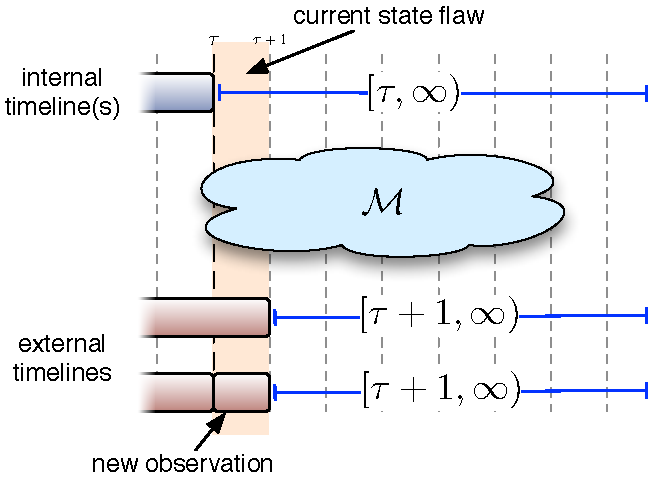
\includegraphics[width=0.5\columnwidth]{figs/synch-relation}
  \caption{Ilustration of the synchronization flaws in a reactor. The
    reactor receive new observations when they are produced by the
    owner(s) of its internal timelines. The line after the last token
    of each timeline represent the domain of possible values for the
    end of this token. At every tick $\tau$ the reactor needs to
    integrate the {\em External} state information it received and --
    based on its model $\mathcal{M}$ -- resolve its {\em Internal}
    state that will then be provided by the architecture to other
    reactors using these state variables.}
  \label{fig:synch:flaw}
\end{figure}

The resolution of internal state flaw can be resolved using one of the
following choices which are evaluated in the given order:
\begin{enumerate}
\item Extend the previous state value to end after this tick (ie
  restrict its end time to $[\tau+1, \infty)$). 
\item Start the next active token in the timeline and
  attempt to start it now (ie restrict its start time to the single
  value $\tau$).
\item Create and insert a new token in this timeline that will start
  at the current tick $\tau$ (attempt this for each possible token
  type for this timeline if necessary). 
\end{enumerate}

All of these choices are evaluated sequentially until a consistent
solution with no more flaw for this tick is identified. In order to do
so we need to make the assumption that the current state value of an
internal timeline do not depend on the future or more accurately
that any choices made during this synchronization will not lead to a
future inconsistency (meaning no possible solution) for a future
synchronization. Such assumption deeply impact the set of possible
domains one the reactor can support while remaining complete. Take for
example the following model rule where {\tt Vehicle} is {\em Internal}
and {\tt Command} is {\em External} to the reactor.
\begin{verbatim}
Vehicle::Dive {
  contains(Command.Descend descend);
  descend.start = start + 2;
}
\end{verbatim}

Such model present the issue that the reactor needs at one point to
take the decision to start the token {\tt Vehicle.Dive} and by doing
so it assumes that in {\em exactly} 2 ticks in the future the {\tt
  Command} timeline will change its state to {\tt Command.Descend}. If
this observation does not occur at the given time this implies that
the reactor estimation was wrong leading him to an inconsistent view
of the world. Conversely the reactor can decide to not switch this
timeline to the {\tt Vehicle.Dive} state and observe 2 ticks in the
future that the {\tt Command.Descend} state value. In this case it
would have missed the opportunity to set its {\tt Vehicle} state to
the correct value which may similarly lead (depending on the rest of
the model) to a similar inconsistency it won't be able to resolve (as
TREX enforces that  the past is monotonic).

While this limitation of the system is important to take into account,
it is also important to note that the model snippet we gave here --
while formally acceptable in the general planning problem -- is also
illustrating a bad design for execution in a situated agent. Indeed,
in this model we are tying the current decision to a future outcome
that is {\em External} to the reactor and therefore not necessarily
controllable by this reactor. Therefore we are entailing a part of the
future to past decisions which can lead the system to a dead-end
situation where the model cannot find a correct solution that both do
not conflict with what we claimed in the past and still allow the
planner to find its current {\em Internal} state.


\subsubsection{Deliberation : planning for future state evolution}
\label{sec:arch:plan}




\subsubsection{Intertwining synchronization and execution }
\label{sec:arch:intertwine}




% Gives a high-level overview of T-REX, the general design principles and how
% these principles aid in software engineering. Show T-REX block diagram.



%%% Local Variables: 
%%% mode: latex
%%% TeX-master: "setobook"
%%% End: 


\section{Experimental Results}
\label{sec:results}

% Show some of the results of the use of T-REX to convince people that is for
% real. CANON will be the predominant driver of the work.


\begin{figure}[htpb]
\centering
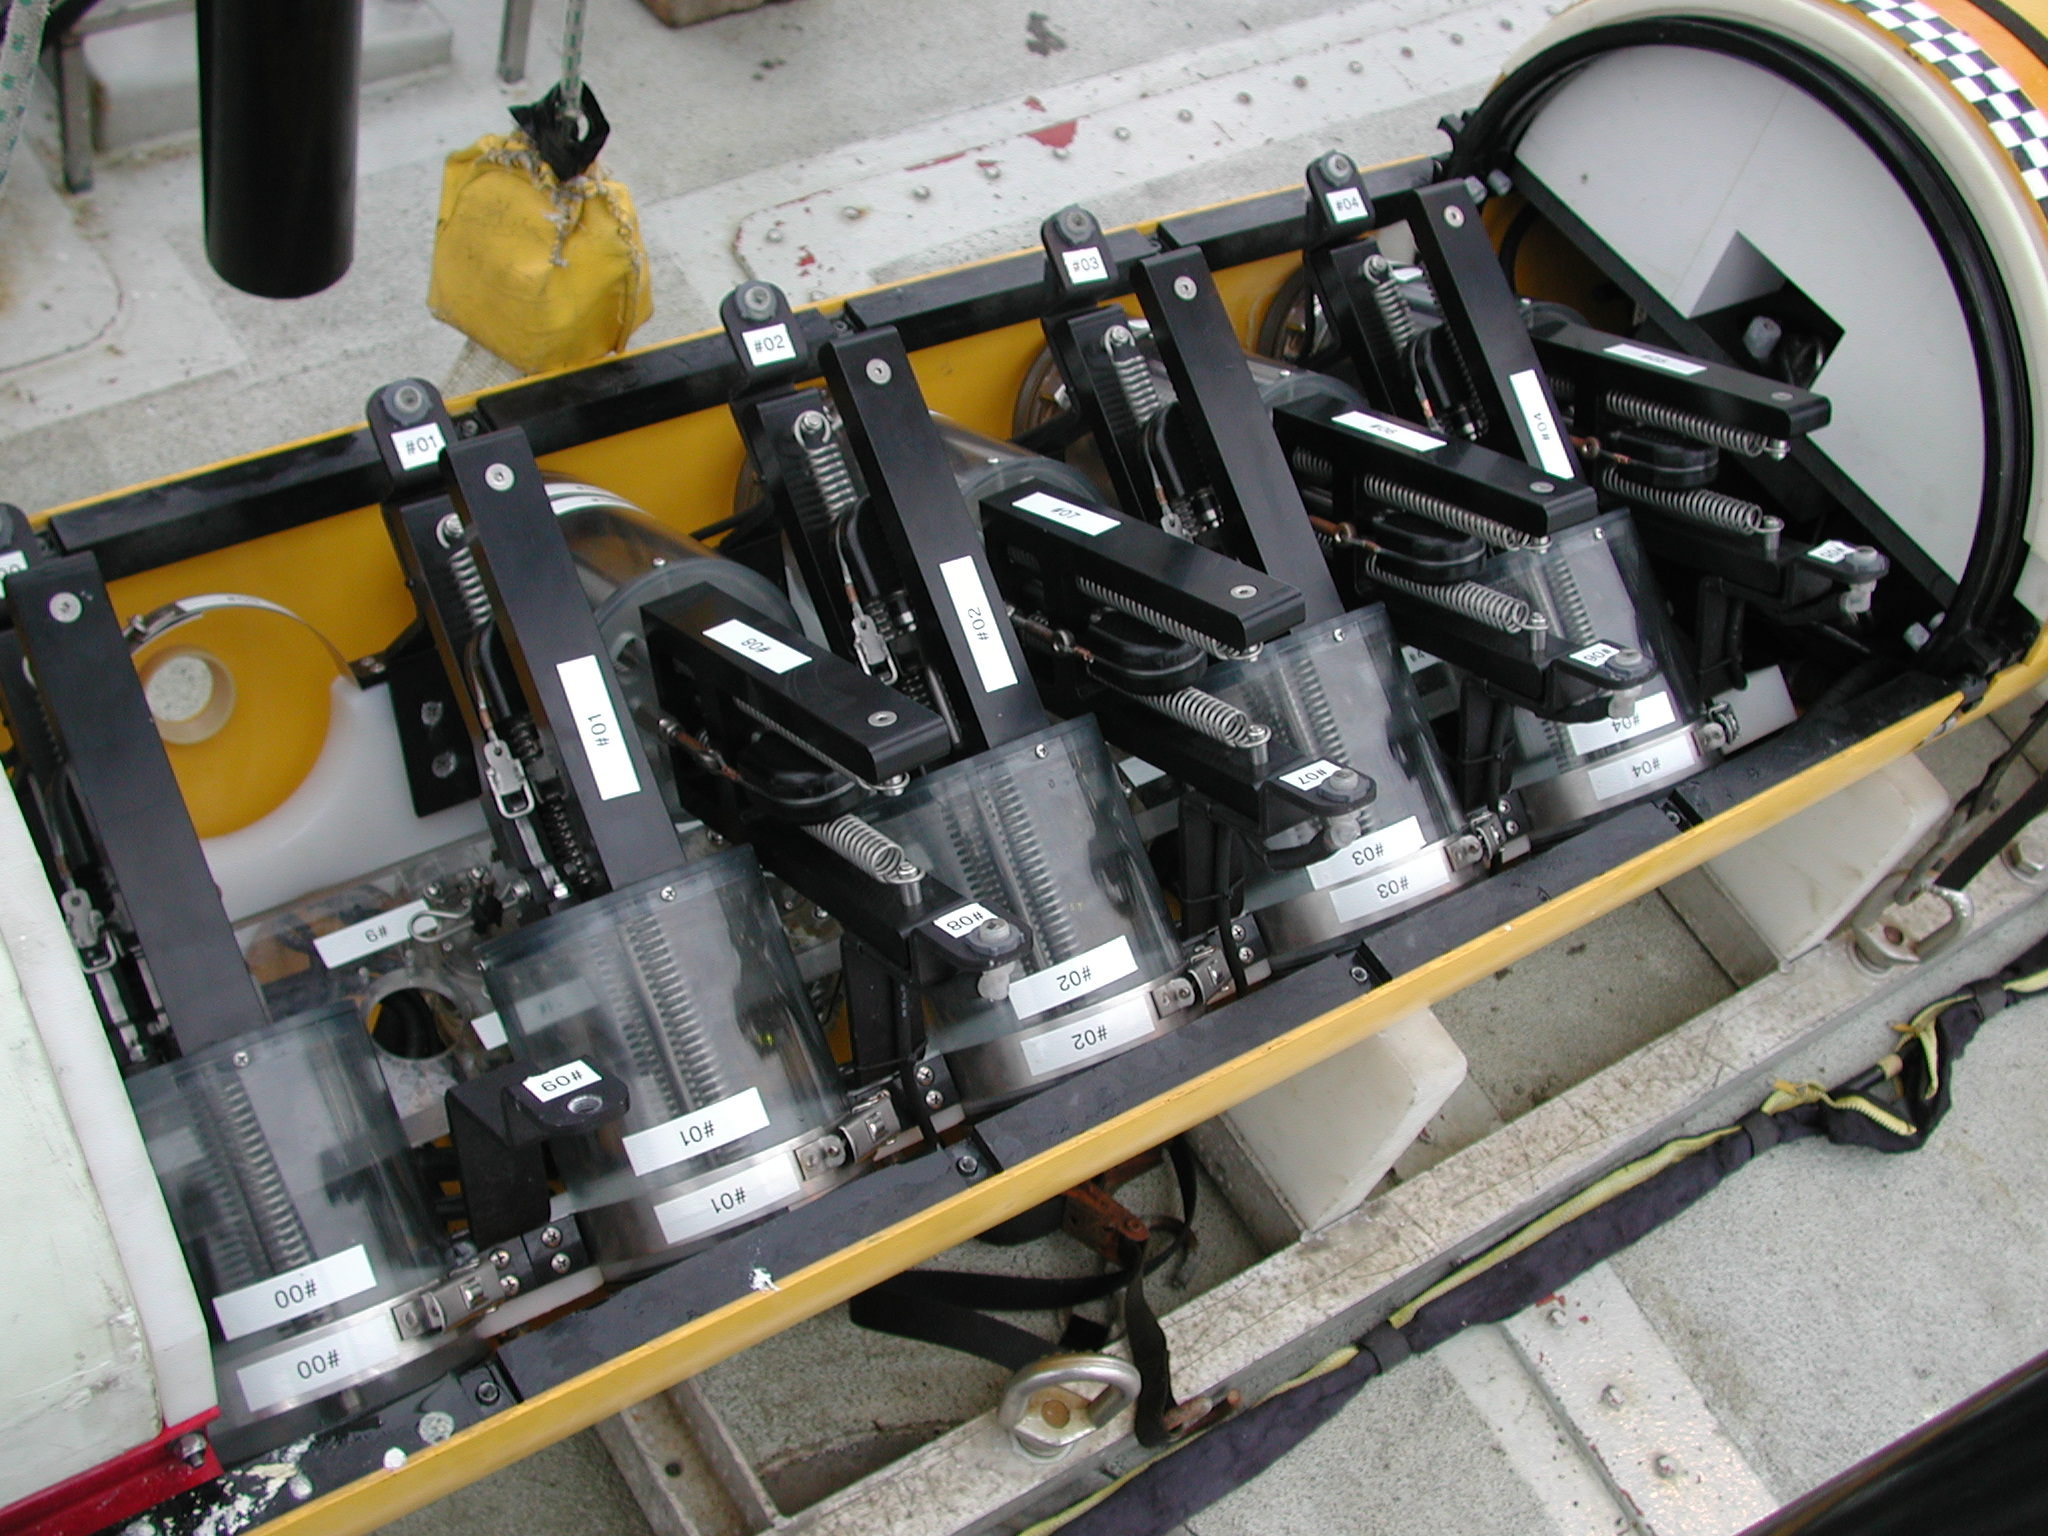
\includegraphics[width=0.35\textwidth]{figs/gulper.jpg}
\caption{\small{The Gulper water sampler \cite{Bird07} on MBARI's
    upper water-column Dorado AUV.}}
\label{fig:gulper}
\end{figure}

A significant driver of the applicability of our work was the
growing need for AUVs mission to be driven by scientific sensor 
data.This trend is illustrated by the 
implementation of MBARI's \emph{Gulper} water-samplers \cite{Bird07},
$2$ litre syringe style containers $10$ of which are encased within
the mid-body section of our Dorado vehicle as shown in Fig
\ref{fig:gulper}. However, the original design and intended use of
operation continued to dominated by a naive belief of collecting and
returning water samples as traditional ship-borne methods often
employ, namely using pre-scripted methods, albeit on a highly capable
robot. With the installation of \rx onboard the Dorado with its
capability to synthesize plans and replan on the fly, more imaginative
methods of sample acquisition were targeted.

Our early work focused on observing and sampling within Intermediate
Nephaloid Layers (INLs) \footnote{INLs are fluid sheets of suspended
  particulate matter that originate from the sea floor
  \cite{mcphee-shaw2006}} \cite{ryan10}. The location and scale of
INLs in the water column, which depend upon seasonal and episodic
variability, are not predictable. In turn, they can be identified by
their high turbidity and low chlorophyll fluorescence. Initial
objectives focused on ways to enhance survey results by ensuring as
large a coverage as possible so that INL fields were observed at
tighter spaced transects and when no INL is detected, then transect
spacing in the lawn mower can be incrementally increased. Follow on
work directly targeted sample acquisition within INLs which are often
sparse, patchy in large horizontal scales (in Kms) and small vertical
scales (in meters). Fig. \ref{fig:inl} shows one example from an AUV
transect from 2005. The intent of both observation and sample
acquisition was to interrupt the nominal plan-execution cycle and
inject an action to alter and re-factor the plan dynamically; in one
instance altering the navigation, the other in actuating a sampler.

\begin{figure}[b]
\centering
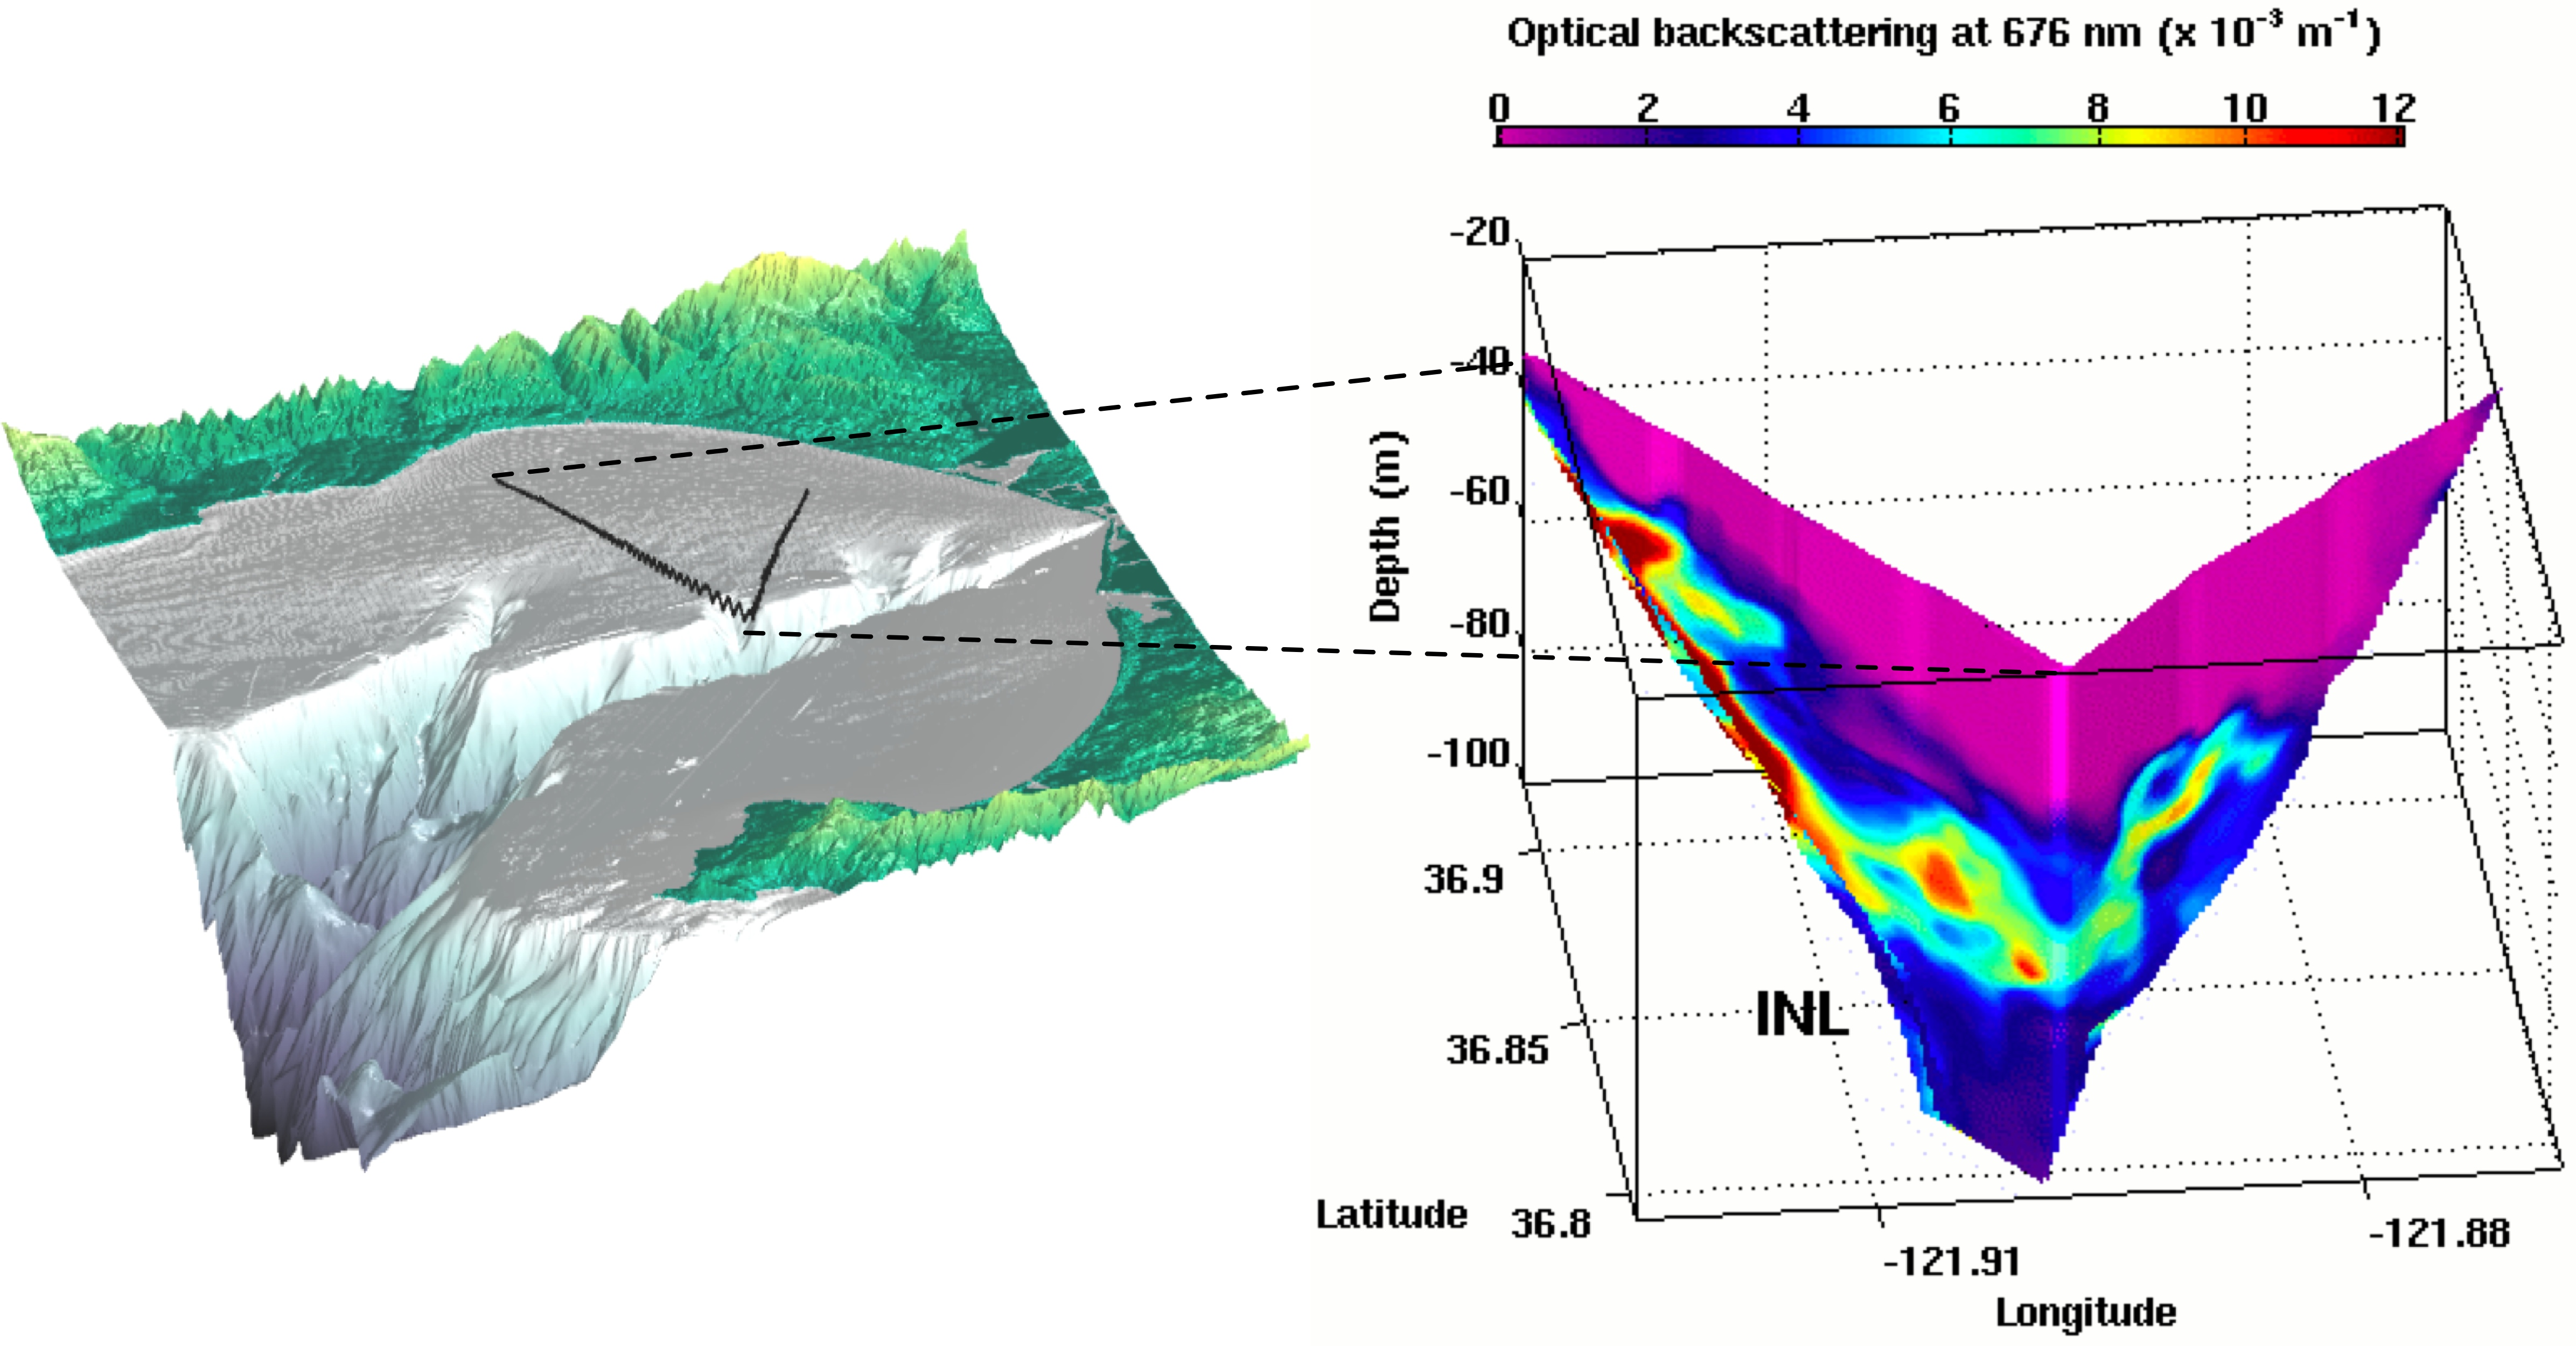
\includegraphics[scale=0.65]{figs/inl.jpg}
\caption{\small An Intermediate Nepheloid Layer (INL) detected by an
  AUV mission in the Monterey Bay in August 2005, showing the location
  of the AUV transect in the bay (left) and optical backscatter image
  at the 420 Nm frequency showing the INLs patchy nature
  (right). \emph{Image courtesy: John Ryan, MBARI}}
\label{fig:inl}
\end{figure}

The implied assumption of installing the samplers on an AUV was that
robotic methods to actuate sample acquisition (with no human control),
would be competitive with human knowledge of where and when to sample
a feature given available shipboard data. To support this assumption,
it required new ways to couple sample acquisition with AUV navigation
and control. While some simple and ad-hoc approaches \cite{yanwu10,
  yanwu11} have shown promise, these techniques were tailored to solve
a specific problem with assumptions on feature structure.  Our
approach on the other hand, stemmed from the need to build a coarse
grained computational model of the INL feature where none existed and
to use that model as a basis to close the \emph{sense-sample-acquire}
loop within the AUV. \cite{fox2007} documents earlier work in using a
well-known unsupervised method in classification the \emph{Kohonen
  Network} or Self-Organizing Maps (SOM) \cite{kohonen} to
\emph{reactively} acquire samples with plan alteration. In doing so we
couple the immediacy of feature identification which is necessarily
reactive, with the deliberation of an onboard temporal planner to
actually trigger a sampler. This has two benefits. First, it goes to
the core of having a deliberative approach to mission planning by
balancing the immediate with that which is projected. Doing so allows
a more systematic approach in dealing with spatial factors in sampling
large volumes. Second, it allows other sampling parameters which are
not directly impacted by perception to be brought to bear; in our
case, scientists would like to introduce constraints (spatial
separation, feature bias, distribution of samples when tracking
multiple features). These are critical not only for science but for
informed decision making which pure reactive approaches simply cannot
undertake.

While the early experiments in \cite{fox2007} coupled the classifier
with the onboard planner, two further novel extensions to sampling
were added. First, to enhance the classifier model by adding a
temporal dimension with a Hidden Markov Model (HMM) \cite{rabiner86,
  Rabiner89atutorial}.  An HMM is a sequential state transition model
in which the current state is not directly visible, but an
observation, dependent on the state, is.  Each state has a probability
distribution over the possible observations.  Therefore the sequence
of observations gives some information about the sequence of traversed
states in the HMM. Unlike identification models based on the simple
classification scheme, HMMs use the dynamics of transition between
modeled states to exploit sequential information of the sensor
readings providing more robust formulation for environmental state
identification. The temporal probabilistic transition then acts as a
filter on top of the clustering model since it is not only derived
from it, but it informs the planner of a potential trigger state only
when the models' transition occurs to an appropriate state of
recognition of the INL feature \cite{mcgann08b}. Not only was
deliberation aided by direct perception of the state (of the INL) but
temporal transition functions added a further level of validation
between expected states in the INL model. This coupling of Machine
Learned model with a deliberative planner is novel in the ocean
sciences and is a continuing direction of investigation \cite{kumar11,
  sergio12}.

The second innovation involved dynamic resource allocation associated
with the water samplers \cite{olaya11}. Using a priori sample
utilities coupled with temporal and spatial information maintained by
the deliberating planner in-situ, the algorithm dynamically generates
a policy on sample acquisition during the course of the mission. In so
doing, utility functions can be used to balance sparcity or abundance
of the feature encountered with the availability of samplers
dynamically. Coupled with periodic sub-sampled science data returned
by the vehicle when on the surface and goal-oriented commanding with
\rxe, such a capability allows judicious use of the limited samplers
by a scientist from her desktop.


\paragraph {Mixed-Initiative Frontal Tracking:} We exploit the
in situ decision making capability of \rx in order to find and
continuously map a thermal gradient. The strategy encapsulated in
algorithms onboard is described by the following three phases:

\begin{figure}[b]
\centering
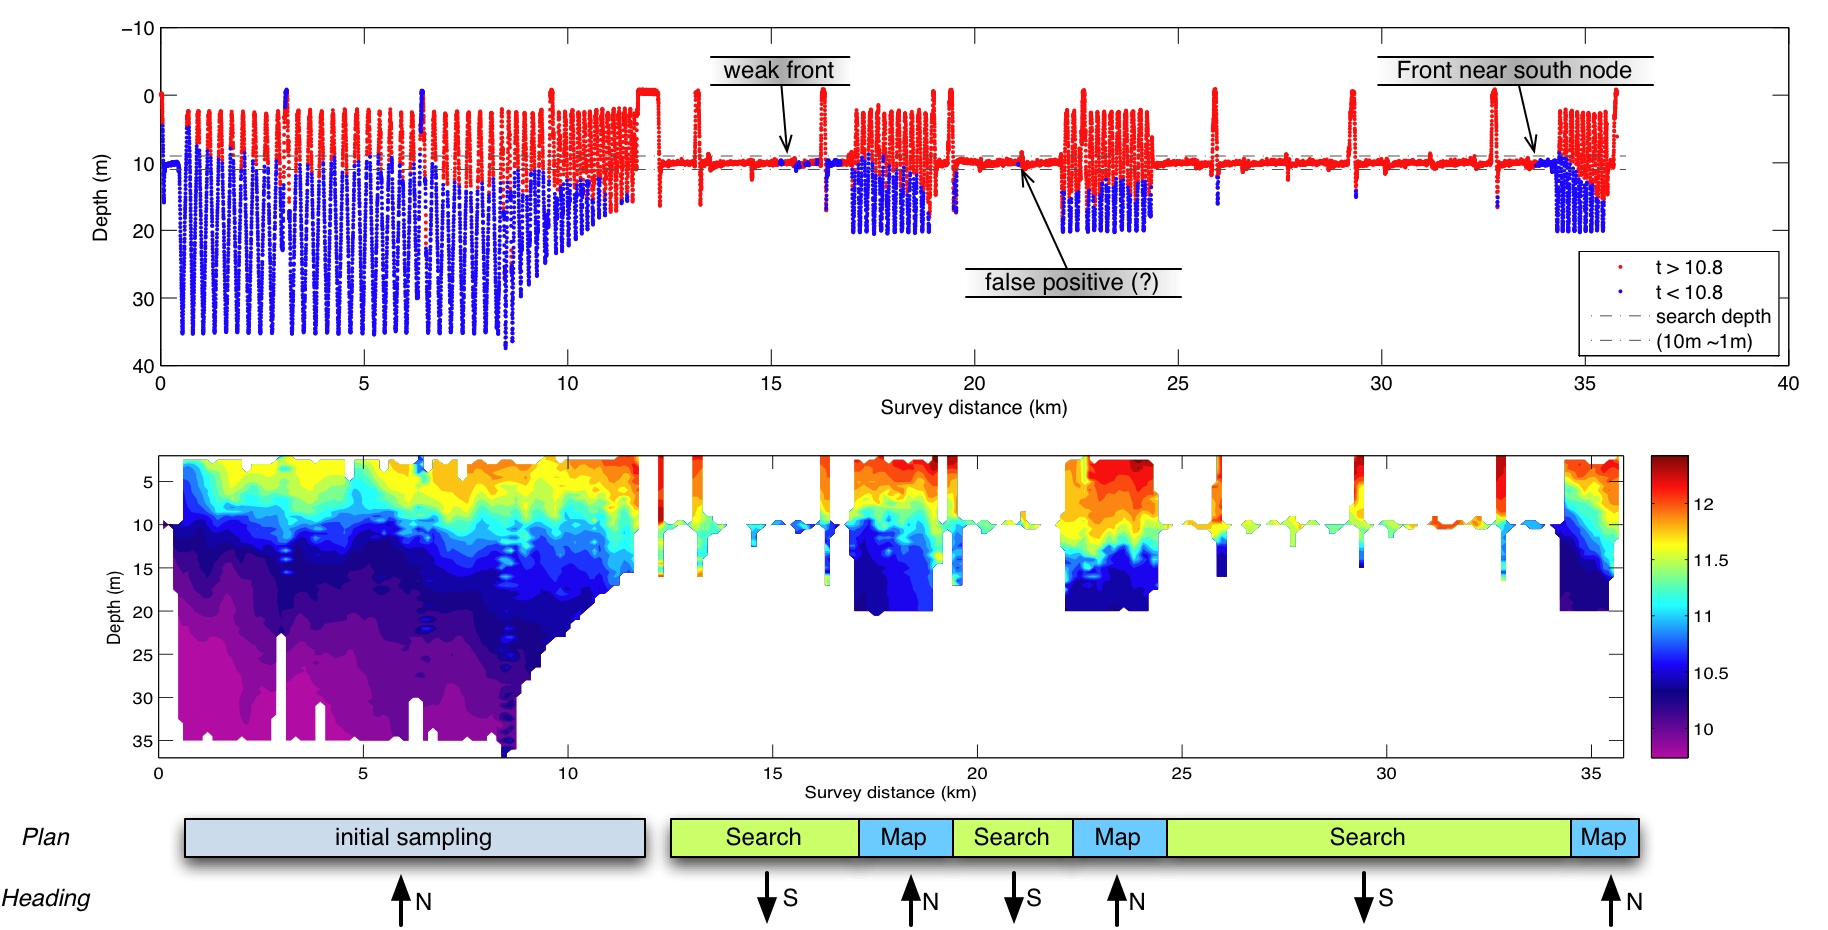
\includegraphics[width=0.8\textwidth]{figs/front-mi.jpg}
\caption{\small{Survey trackline of AUV following a thermal
    gradient. Image in the middle shows the temperature while the
    bottom figure shows different phases in the algorithm.}}
\label{fig:mi-front}
\end{figure}

\emph{Mapping}: The vehicle performs a yo-yo transect between two
designated waypoints and sends temperature sampled every $5$ meters to
shore via satellite. The temperature field is reconstructed from
interpolation of the transmitted data, and the scientist identifies
the target front. Using a graphical user interface, she is then able
to generate a high-level command which represents the front as a
temperature threshold ($t^{\circ}$) at a given depth ($d$). This goal is
then appropriately packaged and sent to the AUV via satellite.

\emph{Search}: After the mapping phase and on receipt of this message
on the vehicle T-REX evaluates the goal, automatically synthesizes a
set of waypoints by generating a plan and then dispatches the plan to
execute by having the vehicle swim back and forth at depth $d$ all the
while reactively evaluating when a temperature threshold $t^{\circ}$
is crossed. In the process \rx checks both the depth and temperature
sensed by the AUV; when the depth is around $d$ ($\pm 1$ meter to
account for vehicle control uncertainty), it then compares the
temperature read with $t^{\circ}$. When the comparison value changes \rx
assumes that the front is identified and switches into the next phase.

\emph{Sampling}: The vehicle undertakes a small transect around the
identified front location while actuating water samplers, one at the
center of the front with temperature threshold $t^{\circ}$, and one on
either side of the front. When this transect is completed, \rx
switches back to the Search phase to follow the frontal evolution.
The survey is completed either when we reach the maximum mission
duration or the vehicle returns to its initial waypoint during the
search phase without crossing the threshold $t^{\circ}$. The latter is
indicative of the frontal zone having left the survey domain.

The novelty in this application was two-fold; in enabling the
deliberation to decide when to trigger the phase changes and in
showing viably how a human being coupled with a goal-oriented
controller could do problem solving jointly. The approach, is general
and can be adapted to any feature or scalar field.

\paragraph {Lagrangian Surveys:} More recent experiments with \rx
controlling the Dorado AUV have centered on the \can (Controlled,
Agile, and Novel Observing Network) program at MBARI. The fundamental
science goals of the program are related to detecting and tracking of
spatio-temporal coastal ocean features \cite{canon}. The dynamic
features require a robotic platform to move with it, return water
samples from across and within gradients and provide contextual
observations to other drifting instruments. All of these observational
strategies are tied to vehicle adaptation which is intrinsically tied
to deliberation and difficult to accomplish otherwise.

Various adaptation methodologies in \can are still being
investigated; however what has become a critical goal for the program
has been to provide contextual environmental information about water
patches. The form and content of such 'patches' varies; for instance
initial attempts focused on Harmful Algal Blooms (HABs). They have
large spatial ($>$ 50 km$^2$) and temporal (days to weeks) extent and
are visible from space with visible coloring on the ocean surface. The
direct impact of HABs is the introduction of toxins into the marine
(and as a consequence human) food chain. In addition,
\cite{anderson00} and \cite{hoagland06} estimate that the average
economic impact resulting from HABs in the United States has been
$\sim$\$75 million from 1987 to 2000. However, the processes behind
bloom initiation, evolution and collapse is poorly understood in part
due to the complex interactions between microbial communities and the
surrounding environment. As a result, our capacity to assess the range
of potential future scenarios that might result from ocean temperature
changes, acidification, or nutrient shifts is highly limited.

\begin{figure}[t]
\centering
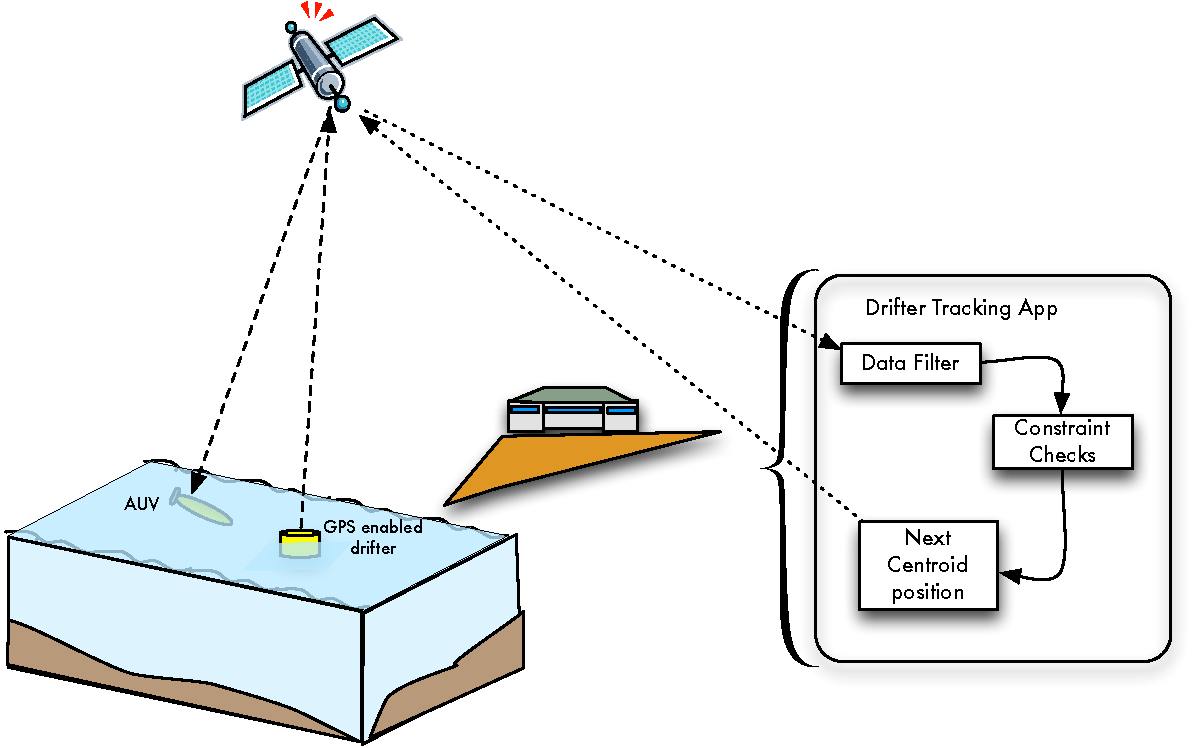
\includegraphics[width=0.5\textwidth]{figs/dta-app.pdf}
\caption{\small{Overall setup of \can lagrangian experiments with a
    drifting instrument pack. Various combinations of computational
    methods can be included in the Drifter Tracking App which is a
    part of the Oceanographic Decision Support System (\od)
    \cite{das11}.}}
\label{fig:dta-setup}
\end{figure}

To augment our understanding of such microbial communities, the Dorado
with \rx has been utilized in a range of activities in a
quasi-lagrangian mode. As the water mass is being tracked with a
drifting instrument, the vehicle is expected to move around it. While
our model suppirt multiples patterns(square, lawn-mower,
transect(s)\dots) with any possible dimension factor, the
majority of at-sea deployments have used a square pattern ($3X3$
km\textsuperscript{2} or a $1X1$ km\textsuperscript{2})\footnote{Often
  post-hoc reconstruction of the data set for visualization drives how
  much adaptation the vehicle can be allowed to undertake.}. Plan
synthesis occurs frequently, but within the context of a drifting
point generated by a drifter. Fig. \ref{fig:dta-setup} shows the
general setup of our experiments which can be tailored with the use of
various computational methods within the \texttt{DTA} app which is
contained within the Oceanographic Decision Support System (\od; see
below) \cite{das11}. GPS data from the free-floating drifter is sent
via satellite and processed onshore to determine a projection (speed
and bearing) of the drifter. This data is sent to the AUV; at the
completion of the current survey, the vehicle receives this data as a
high-level goal which is decomposed and synthesized as a survey
plan. Currently, the vehicle completes the survey without any further
dynamic updates from the drifter. In order to minimize the range of
errors that the survey needs to encapsulate (data latency or surface
or sub-surface currents for those drifters which have a drogue) the
estimation is a projection in time and space of the drifters centroid
sent with this goal from the shore-side app.

\begin{figure}[htpb]
\centering
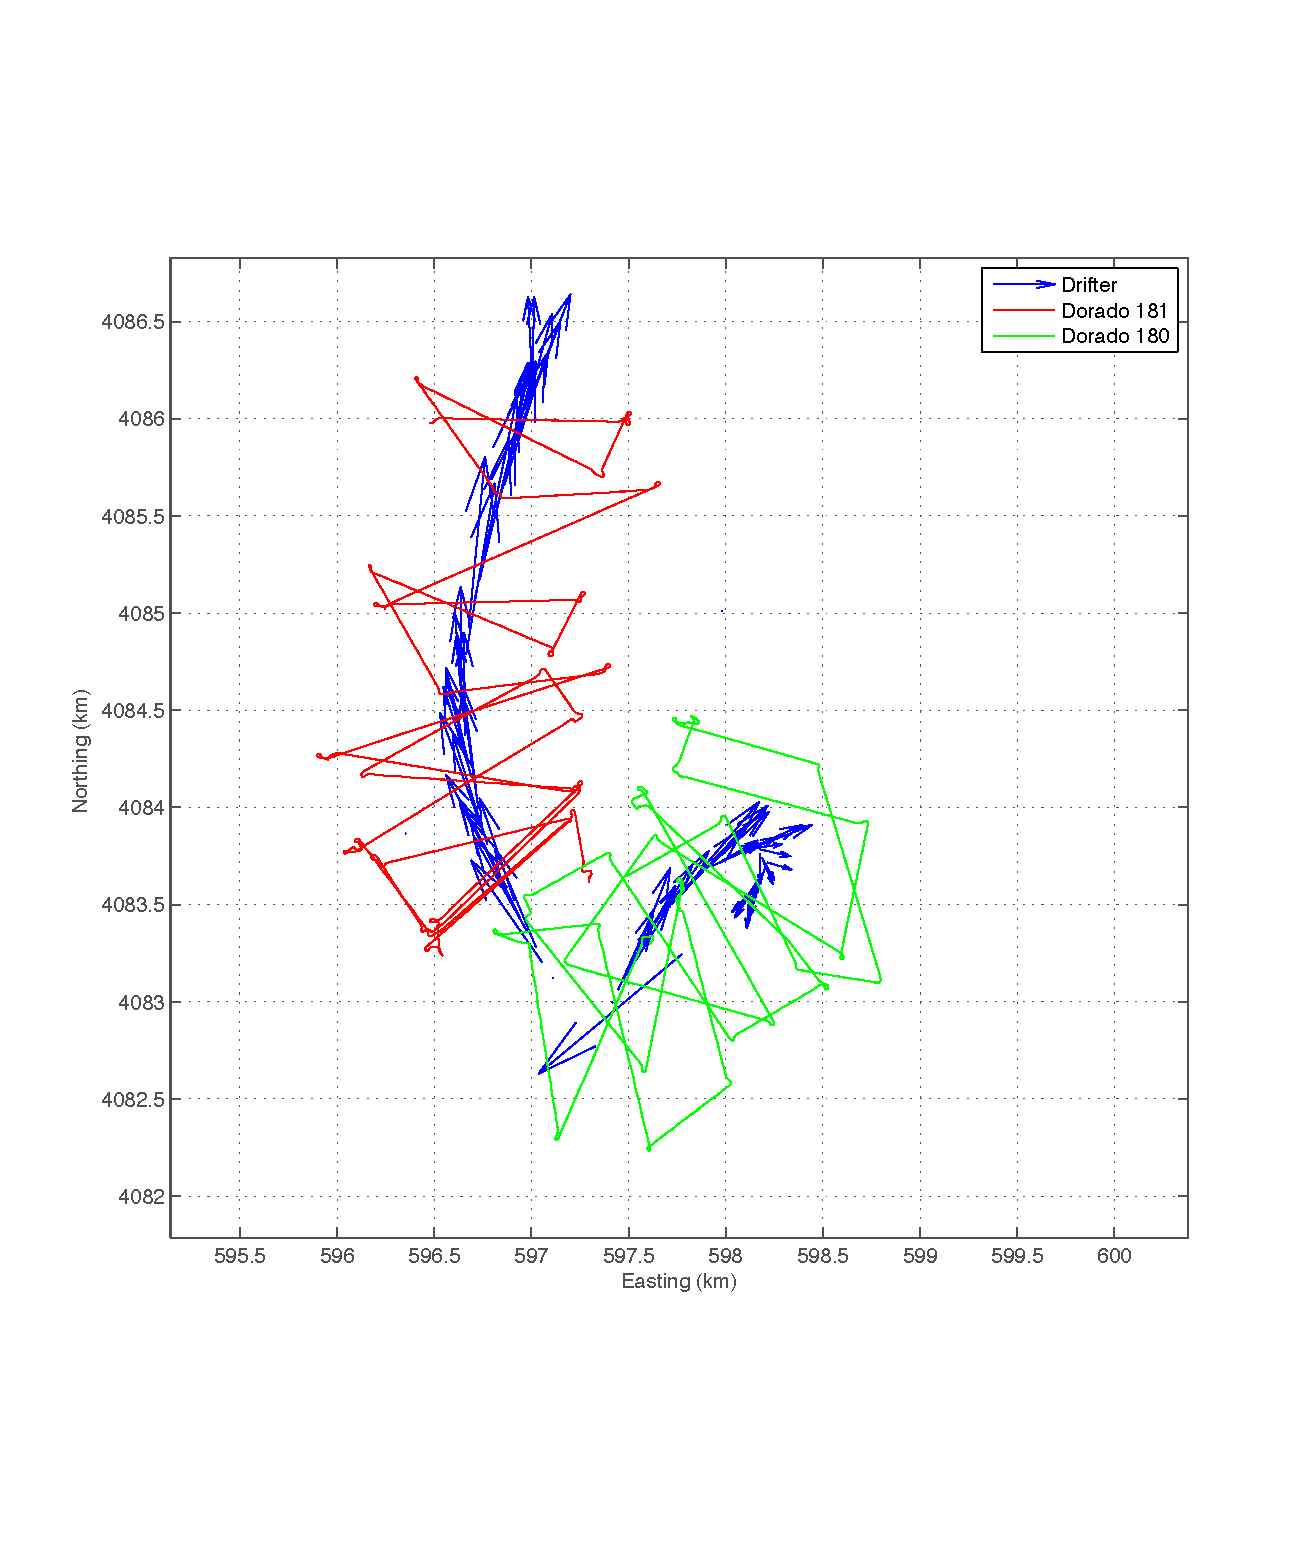
\includegraphics[width=0.35\textwidth]{figs/june11-drifter-follow-180-181.pdf}
\caption{\small{A June 2011 drifter cruise shown in the Earth
    frame. Deviations in the AUV transect are based on the frame of
    reference in addition to positional errors \cite{das11b}.}}
\label{fig:drifter-errors}
\end{figure}

Typically this has meant that the vehicle computes a set of waypoints
for the survey plan, moves to the start waypoint and then executes the
survey even as the centroid is moving. Positional error of the vehicle
and uncertainty in the speed and bearing of the vehicle\footnote{In
  our September 2010 experiment as the drifter moved over the Davidson
  Seamount \cite{clague10} deviation in the California current
  resulted in visible directional change that can be seen in
  Fig. \ref{fig:sep10-transects} at the end of the mission.} exist;
however, the observations of the survey to retain the environmental
context require a change in reference frames so that the patch-center
tagged by a GPS-tracked drifter remains within the survey perimeter at
all times \cite{das11b}.

\begin{figure*}
\centering
\subfloat[]{\label{fig:sep10-ship}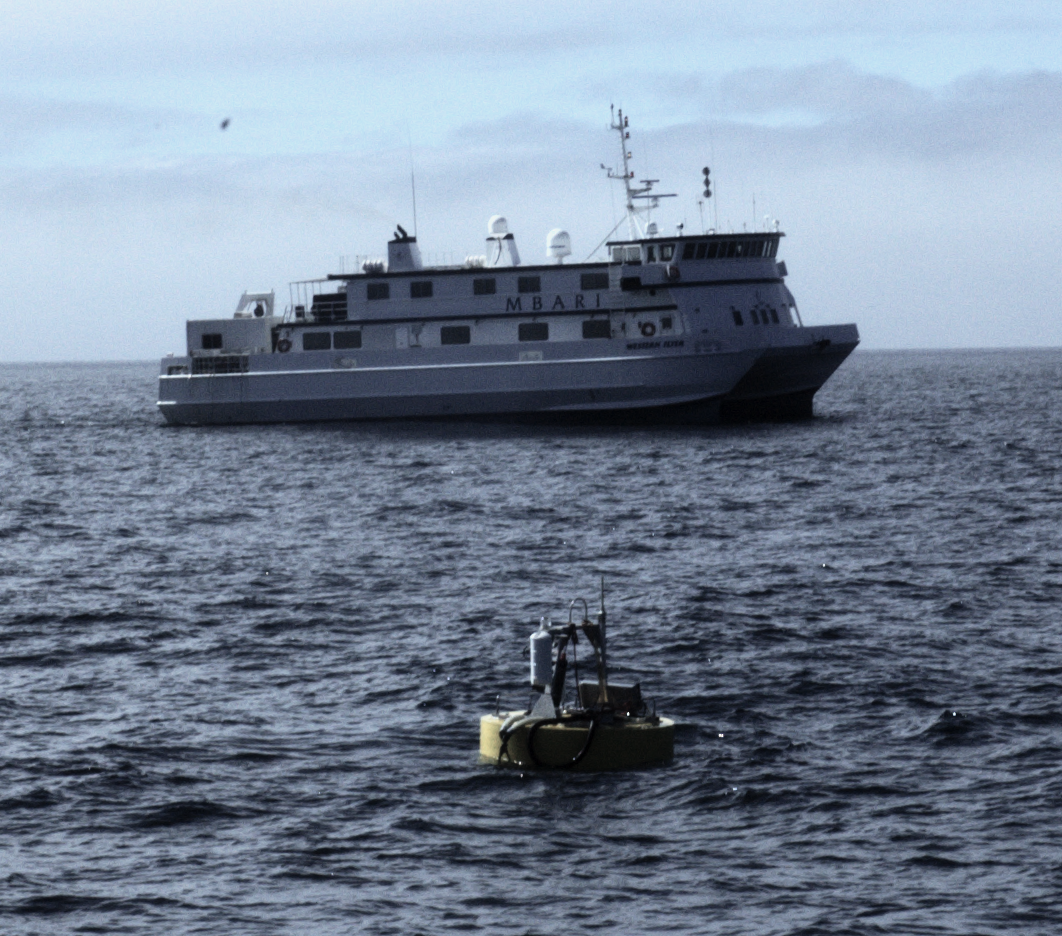
\includegraphics[width=0.38\textwidth]{figs/sep10-canon-cruise.png}}
\subfloat[]{\label{fig:sep10-transects}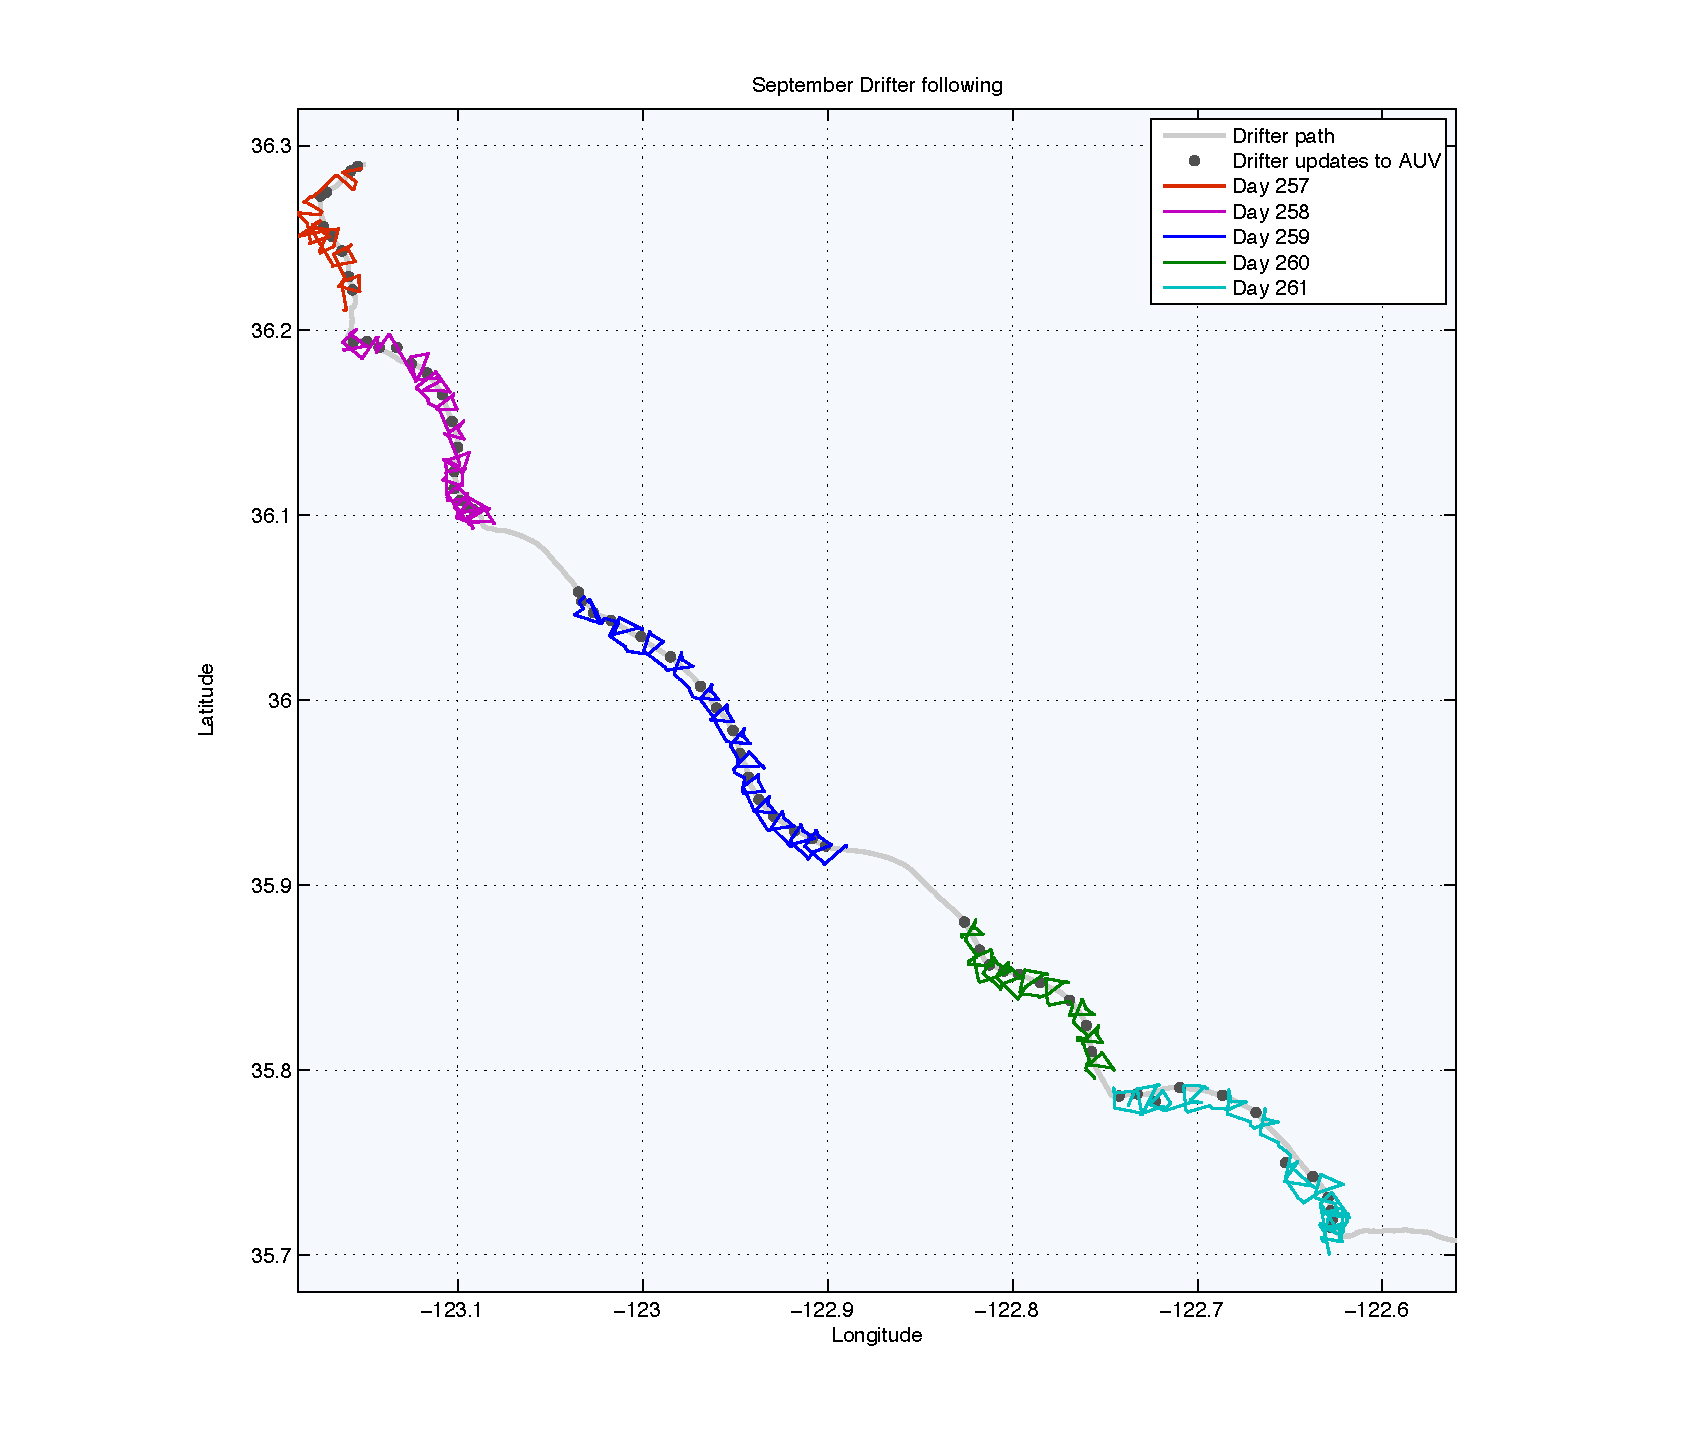
\includegraphics[width=0.35\textwidth]{figs/september-iterations.pdf}}
  \caption{\small{The offshore \can ESP-drifter following cruise
      \cite{das11b}. Fig. \ref{fig:sep10-ship} shows the ESP drifter
      foreground with the R/V \emph{Western Flyer} with the image
      taken from the R/V \emph{Zephyr}. Fig \ref{fig:sep10-transects}
      shows the 86 km transect of the Dorado following the ESP drifter
      about 100 Nm from California shores.}}
\label{fig:gulper}
\end{figure*}

These theoretic results were validated in a five-day long off-shore
deployment carried out in September 2010, 160 kms off the California
coast (Fig.~\ref{fig:sep10-ship}). A specialized drifter with a
genomic sensor \cite{scholin09} hanging $20$ m below, performing
in-situ identification of micro-organisms was the target. The
experiment was supported by crews on two support vessels, the R/V
\emph{Western Flyer} and the R/V \emph{Zephyr}. The \emph{Flyer}
visited the drifter every four hours to carry out a series of
ship-based sampling experiments and lab analysis on water samples to
ground-truth the drifter sensor data. The \emph{Zephyr} was meanwhile
focused on Lagrangian observation studies using the Dorado with the
goal to monitor the nutrient budget at the perimeter of a $1$km $X
1$km water patch around the advecting drifter while the AUV performed
a transformed box pattern around the drifter. A number of logistical
issues were kept in mind while designing and executing the
experiment. Each iteration began with the latest drifter update
(position and velocity) received from the drifter through a satellite
link which was transmitted to the vehicle for in-situ adaptation. \rx
used this input to compute the $5$ waypoints necessary for an
iteration of the box pattern, with the AUV traveling at constant
velocity in the earth frame. Waypoints were computed once at the
beginning of the survey with the AUV surfacing once for every survey,
with each survey lasting $\sim1$ to $1.5$ hours. A total of 60 surveys
were attempted over the course of the $5$
days. Fig. \ref{fig:sep10-transects} shows the overall transects over
the course of the mission, with gaps in between days when the AUV was
being recharged. Each deployment lasted $\sim12$ hours. The black dots
in the figure show the beginning of each iteration when drifter
updates were received by the AUV.


\begin{figure}[t]
\centering
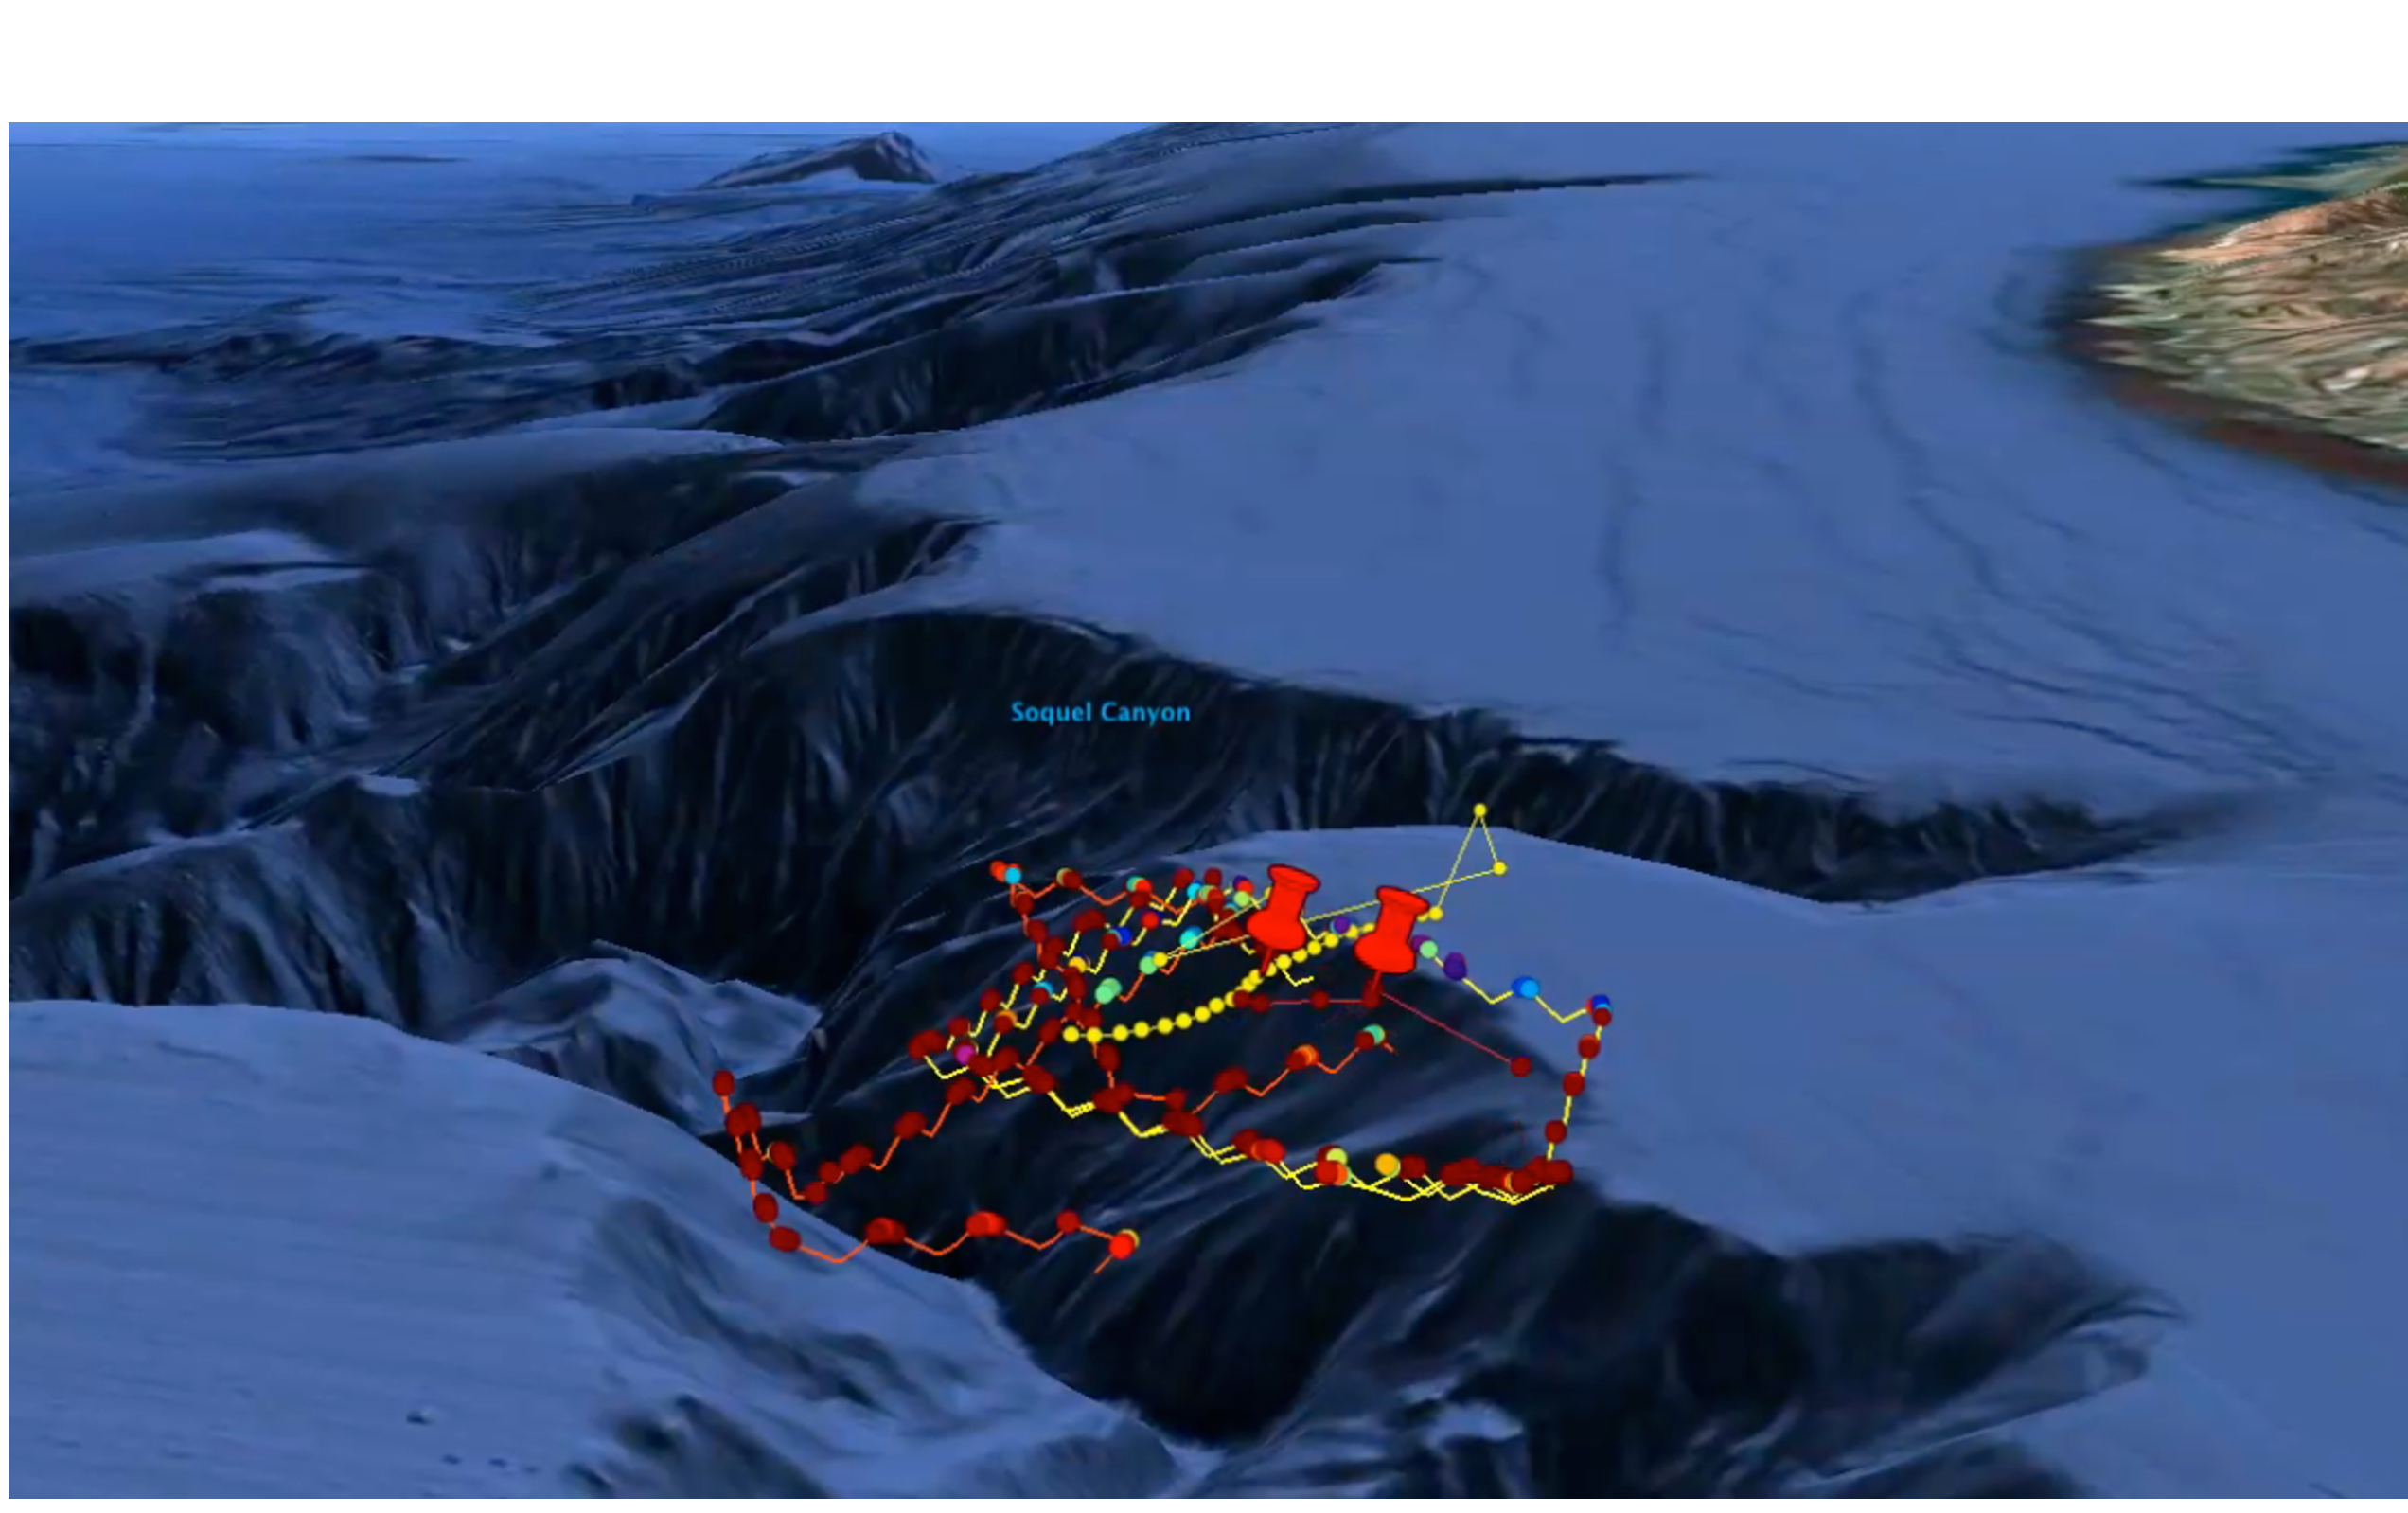
\includegraphics[width=0.7\textwidth]{figs/oct10-ballet.pdf}
\caption{\small An October 2010 robot ``ballet'' where a smaller
  slower AUV tracked a patch center, sending periodic updates to the
  Dorado using a setup shown in Fig. \ref{fig:dta-setup}. The Google
  Earth post-hoc image shows {\color{red}red} track lines of the \rx
  commanded Dorado with the {\color{yellow}yellow} transects of the
  LRAUV. {\color{yellow}Yellow} dots show the track line of a
  GPS-enabled drifter used for seeding the experiment over the
  Monterey Canyon with Santa Cruz, California to the right of the
  figure.}
\label{fig:ballet}
\end{figure}

Successive lagrangian experiments also followed a more innovative and
robotically choreographed ``ballet'' between two AUVs, the Dorado and
the LRAUV \cite{bellingham10} in October 2010 as part of another
series of \can field experiments. The slower vehicle with a
fluorometer tracked a targeted chlorophyll patch seeded by a
GPS-enabled drifter, sending periodic updates of the patch centroid to
shore via the \od following a setup similar to
Fig.\ref{fig:dta-setup}, to the Dorado running \rxe.

\begin{figure*}
\centering 
\subfloat[Temperature]{\label{fig:sep11-temp}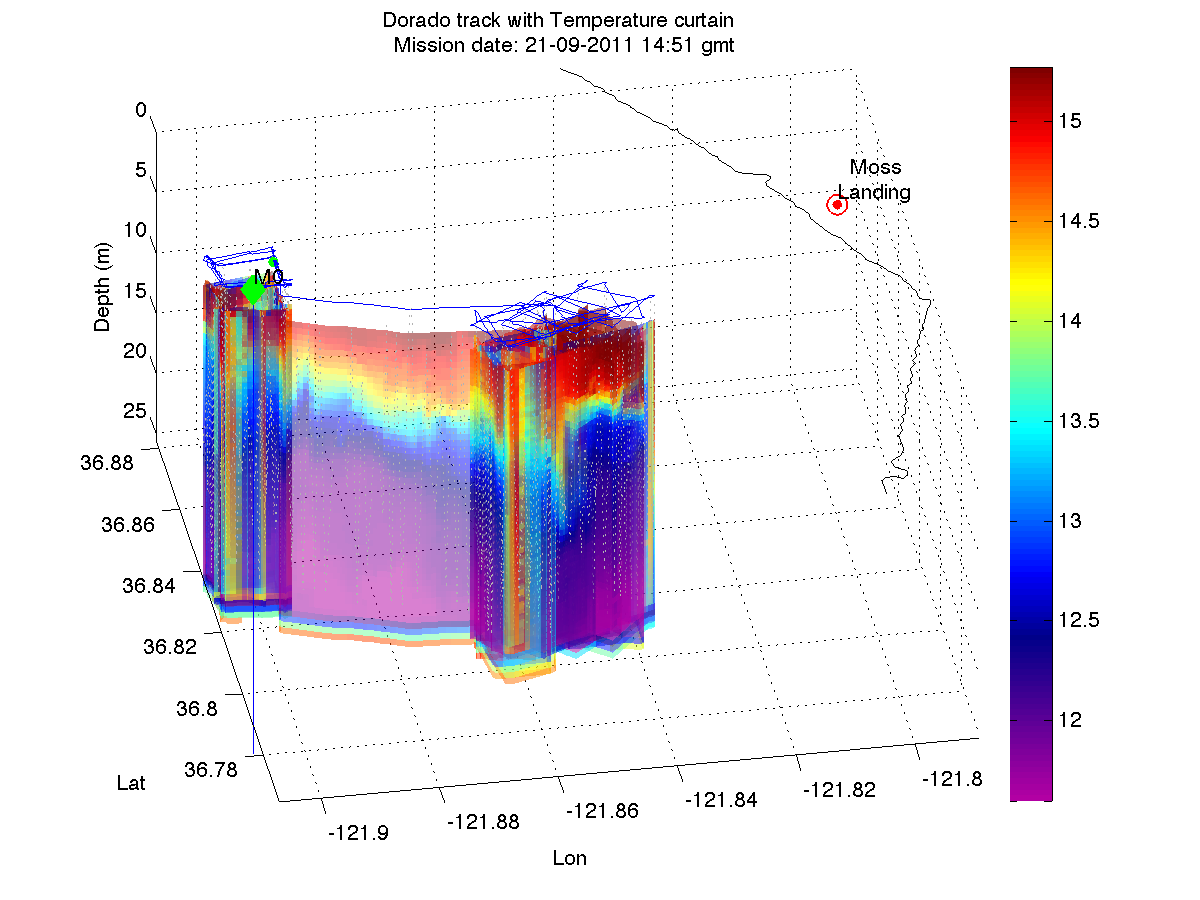
\includegraphics[width=0.5\textwidth]{figs/sep11-ww-temp.png}} 
\subfloat[Salinity]{\label{fig:sep11-sal}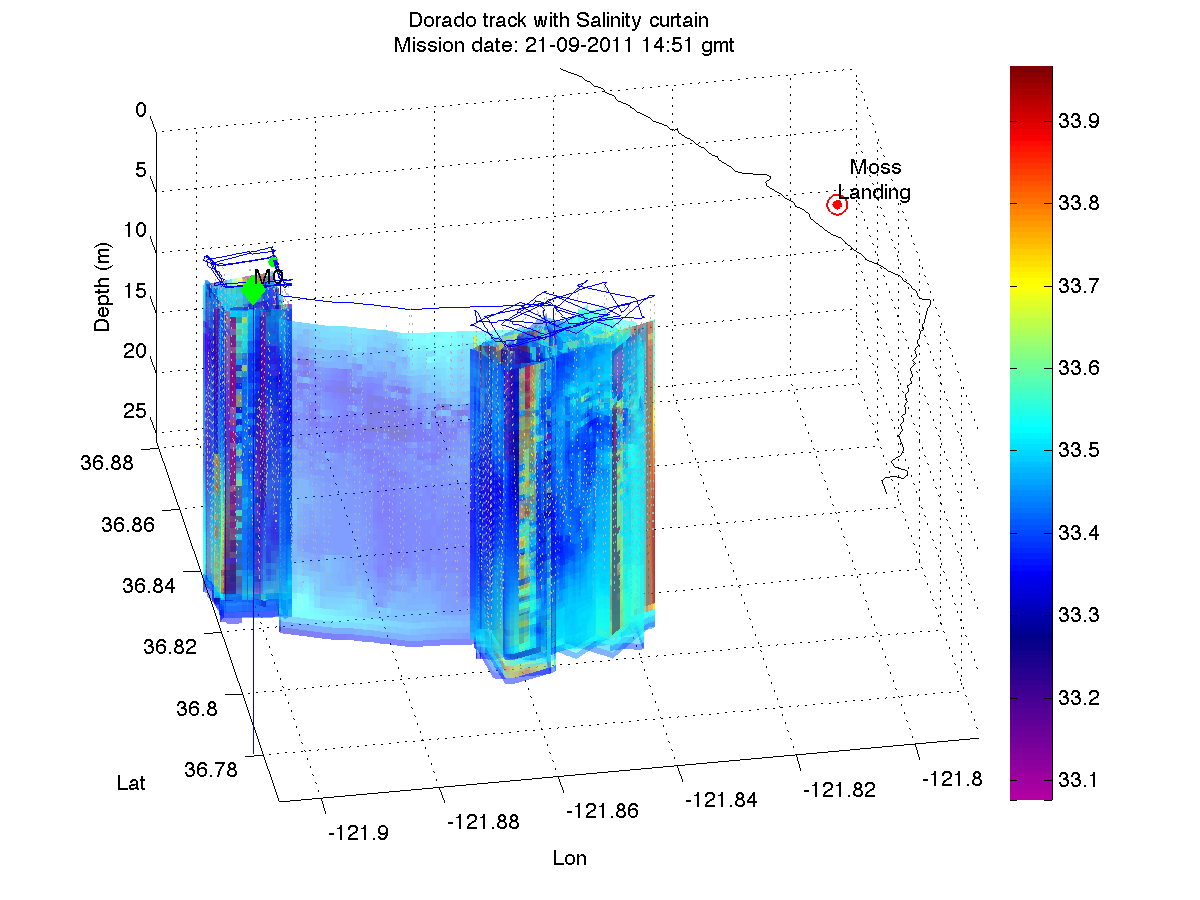
\includegraphics[width=0.5\textwidth]{figs/sep11-ww-salinity.png}}\\
\subfloat[Fluorescence line height]{\label{fig:sep11-flh}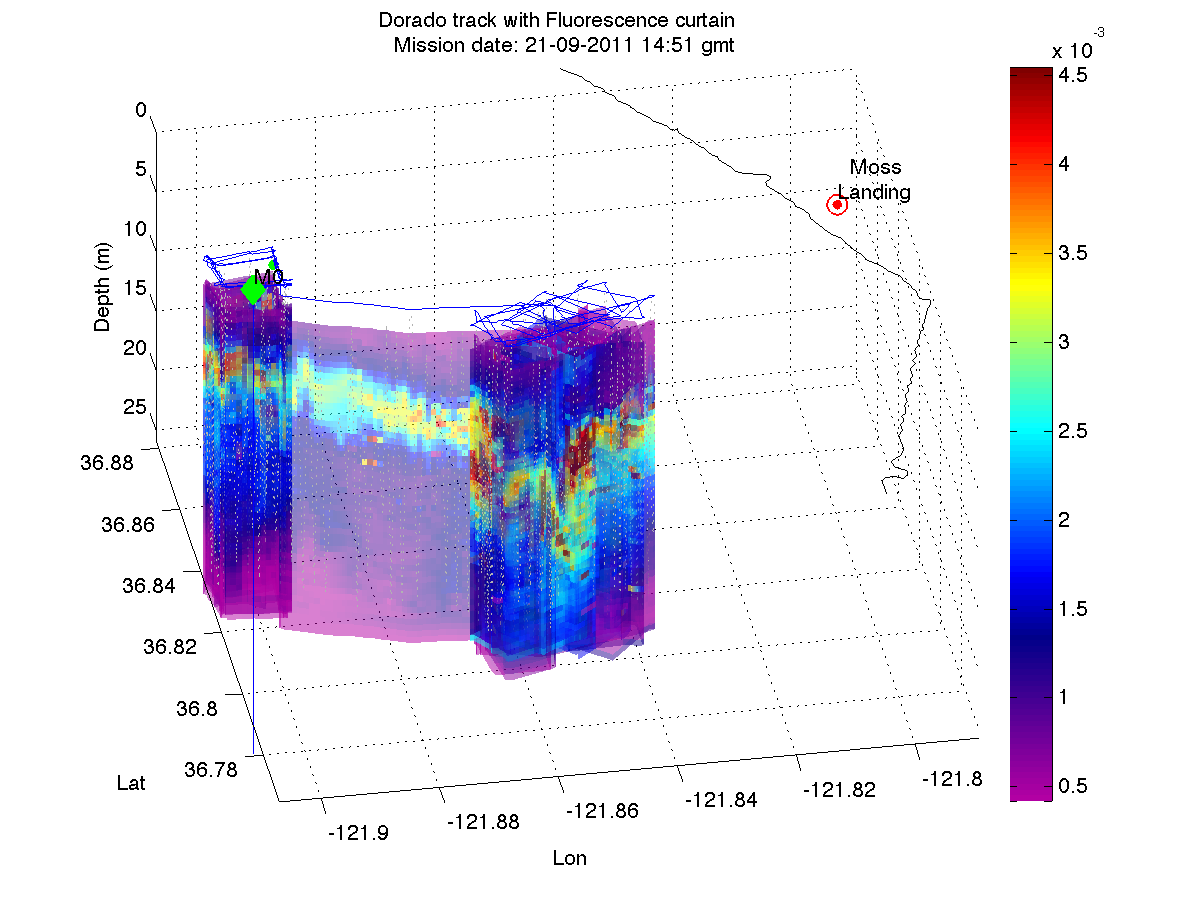
\includegraphics[width=0.5\textwidth]{figs/sep11-ww-flh.png}} 
\subfloat[Nitrate]{\label{fig:sep11-n2}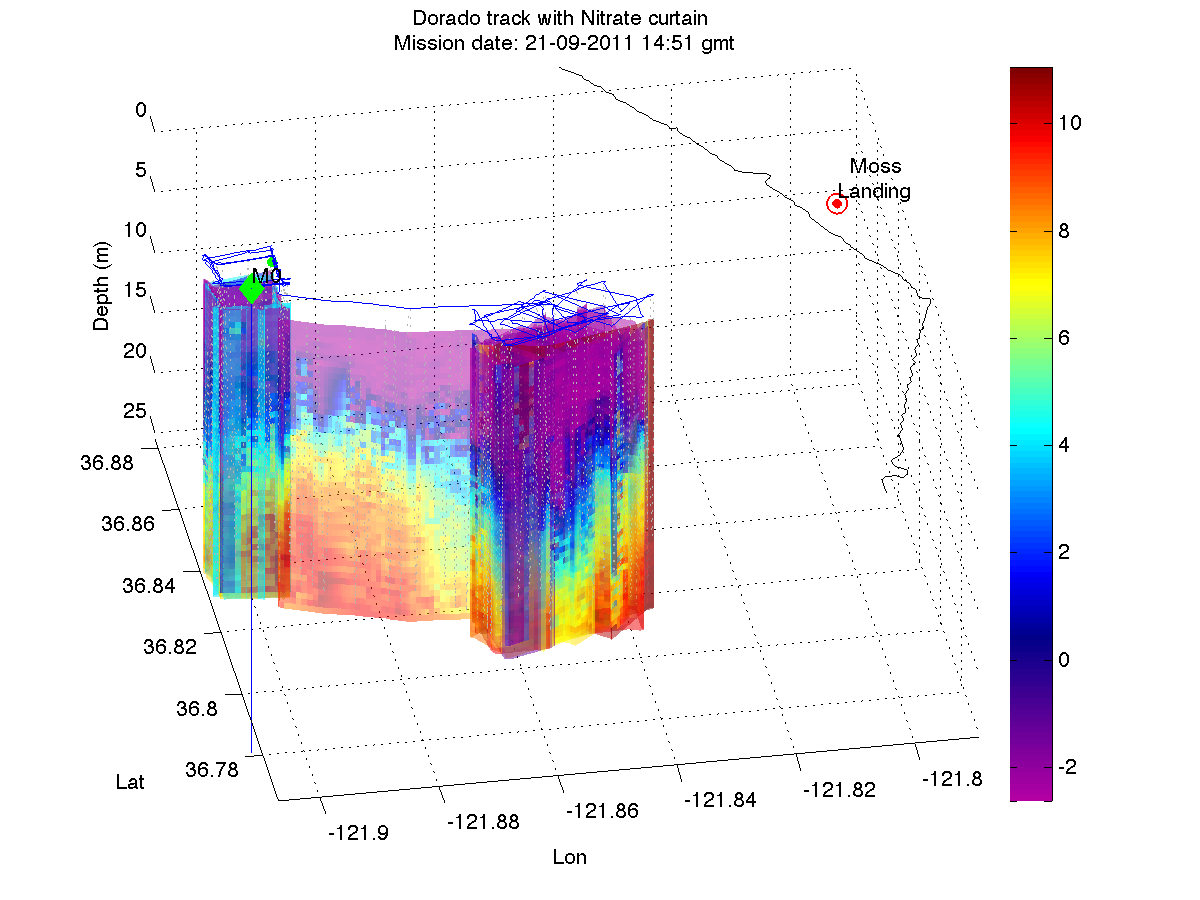
\includegraphics[width=0.5\textwidth]{figs/sep11-ww-n2.png}} 
\caption{\small Interpolated results of a September 2011 \rx mission
  in the Monterey Bay with the profiling \texttt{Wirewalker}
  \cite{rainville01,pinkel11} instrument. Plots show the instrument
  was entrained between two fronts. \emph{Image courtesy: Rishi
    Graham, MBARI}}
  \label{fig:sept11-wirewalker}
\end{figure*}

More interesting experiments are being carried out as a basis to track
more dynamic features such as ocean fronts \cite{fronts11} and
tracking more capable drifting platforms. In particular experiments
with a profiling CTD instrument, the \texttt{Wirewalker}
\cite{rainville01,pinkel11} are resulting in new modalities of making
Lagrangian and Eulerian observations. Fig. \ref{fig:sept11-wirewalker}
shows one such experiment in September 2011 with a GPS-enabled
\texttt{Wirewalker} was tracked by the Dorado running \rxe. We are
currently investigating spatio-temporal correlations \cite{gneiting07}
of CTD data obtained by the \texttt{Wirewalker} and tying it to the
observations made in the contextual environment by the Dorado's
sensors.

\paragraph {Mixed-Initiative Autonomy}

\begin{figure*}
  \centering
  \subfloat[A conceptual view of the \od and how it fits into \can
  field experiments]{\label{fig:odss-concept}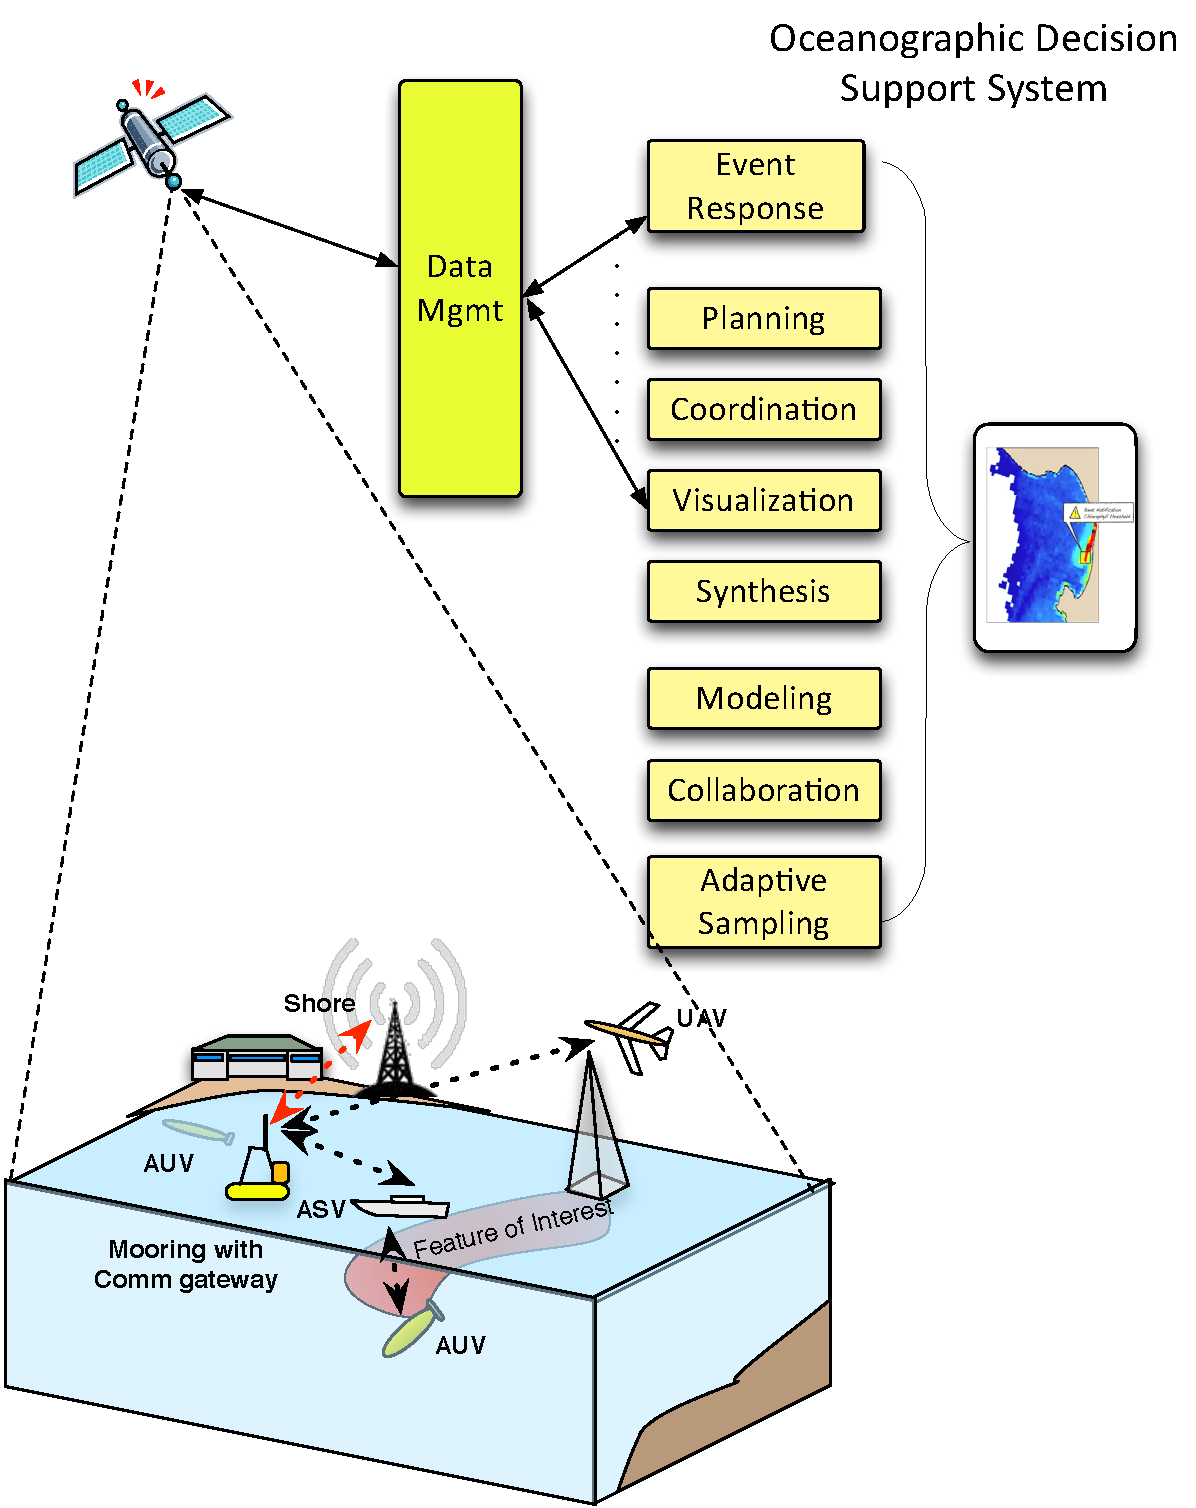
\includegraphics[width=0.5\textwidth]{figs/odss-concept.pdf}}\\
  \subfloat[Current implementation of \od for
  \can]{\label{fig:odss-frontend}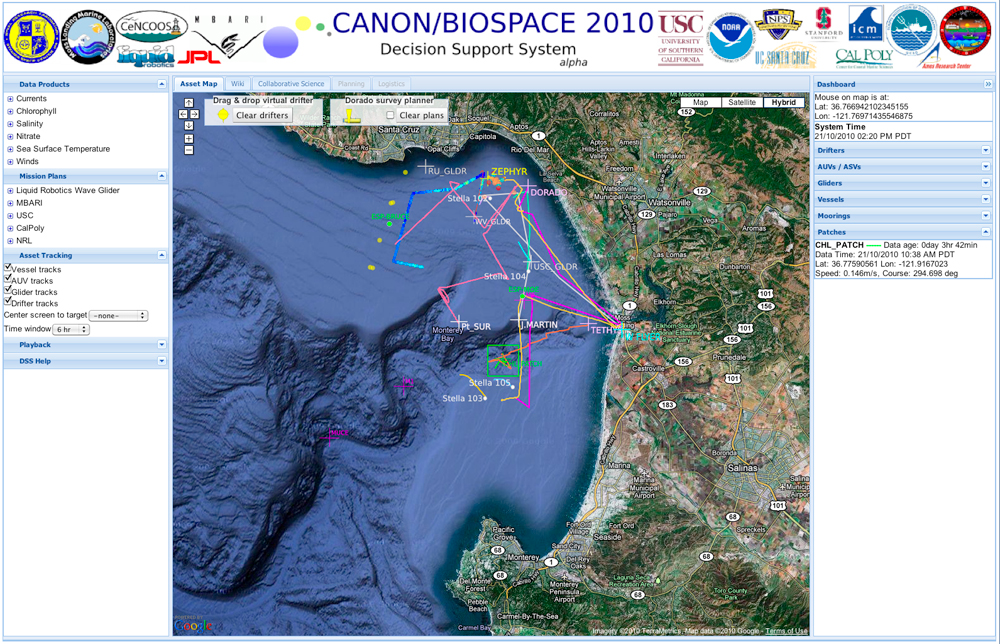
\includegraphics[width=0.5\textwidth]{figs/dss-screenshot.png}}
\caption{\small The Oceanographic Decision Support System (\od) is a
  single portal for planning, visualization, situational awareness,
  collaboration and archival of information before, during and after
  field experiments. The \od has been used since mid-year 2010 for
  \can field experiments.}
\label{fig:odss}
\end{figure*}

Large scale oceanographic field experiments akin to those targeted by
\can are usually logistically constrained driven largely by ship
schedules.  Once a feature set has been identified for scientific
observation and science goals have been collated, the appropriate
robotic assets need to be assigned and deployed for observation and
sampling. This asset allocation in turn depends on parameters like
sensor payload, the speed of the robot \situ in comparison to the
spatio-temporal scales of the evolution of the phenomena being
sampled, the number of assets in a class, the kinds of measurements
needed (e.g synoptic or close-up), logistical considerations for
deployments such as battery charge needed or distance/time to deploy,
impact to long-range deployment plans among others. All drive the
strategy to balance short and long-term scientific and engineering
needs. Our \can deliberations during the 2010 field season for example,
were driven by all of the above \cite{das11}. Often these strategies
were rebalanced during each decision-making cycle, especially in light
of opportunistic science goals. For example, gliders running at $0.5$
knots were often retargeted when surface support vessels noted the
apparent dispersal of the bloom to subsurface layers when HABs were a
\can target. However, their retargeting was carefully
monitored to balance the long-term desire of obtaining time series
within fixed tracks and with the need to ensure these assets were not
exposed to strong currents. Powered AUVs were targeted to chase after
advecting blooms, but the decision on their deployment locations and
survey areas too close to the surf-zone were avoided. In
patch-tracking experiments, the deployment of drifters close to shore
and where depths of $20m$ or less were encountered, was avoided even
when contrary to scientific intent. The need to obtain high-quality
data for post-hoc analysis was also driven by the response time of
data returned by experiment partners.

\begin{figure*}
\centering
\subfloat[]{\label{fig:odss-mtg}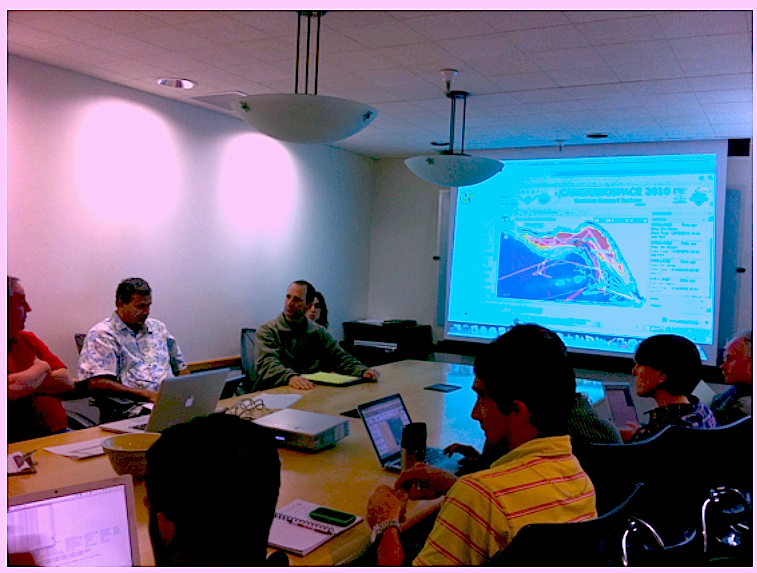
\includegraphics[width=0.3\textwidth]{figs/october-canon-meeting.png}}
\subfloat[]{\label{fig:odss-virtual}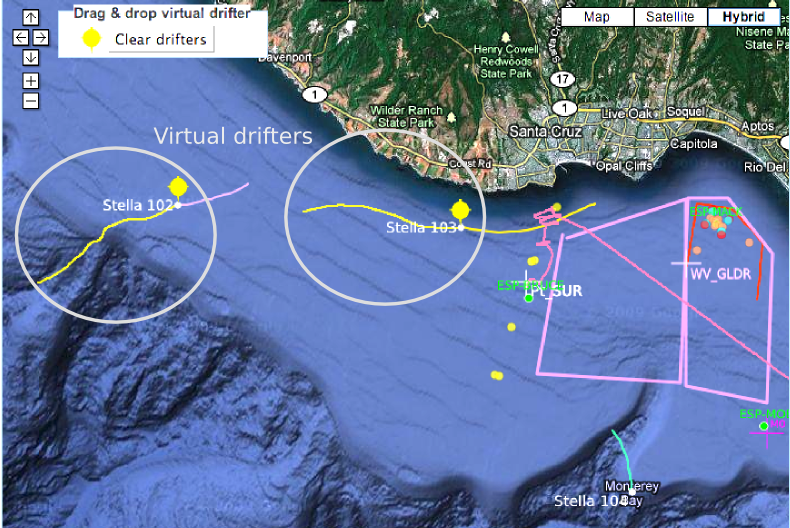
\includegraphics[width=0.33\textwidth]{figs/virtual-drifter-tool.png}}
\subfloat[]{\label{fig:odss-ipad}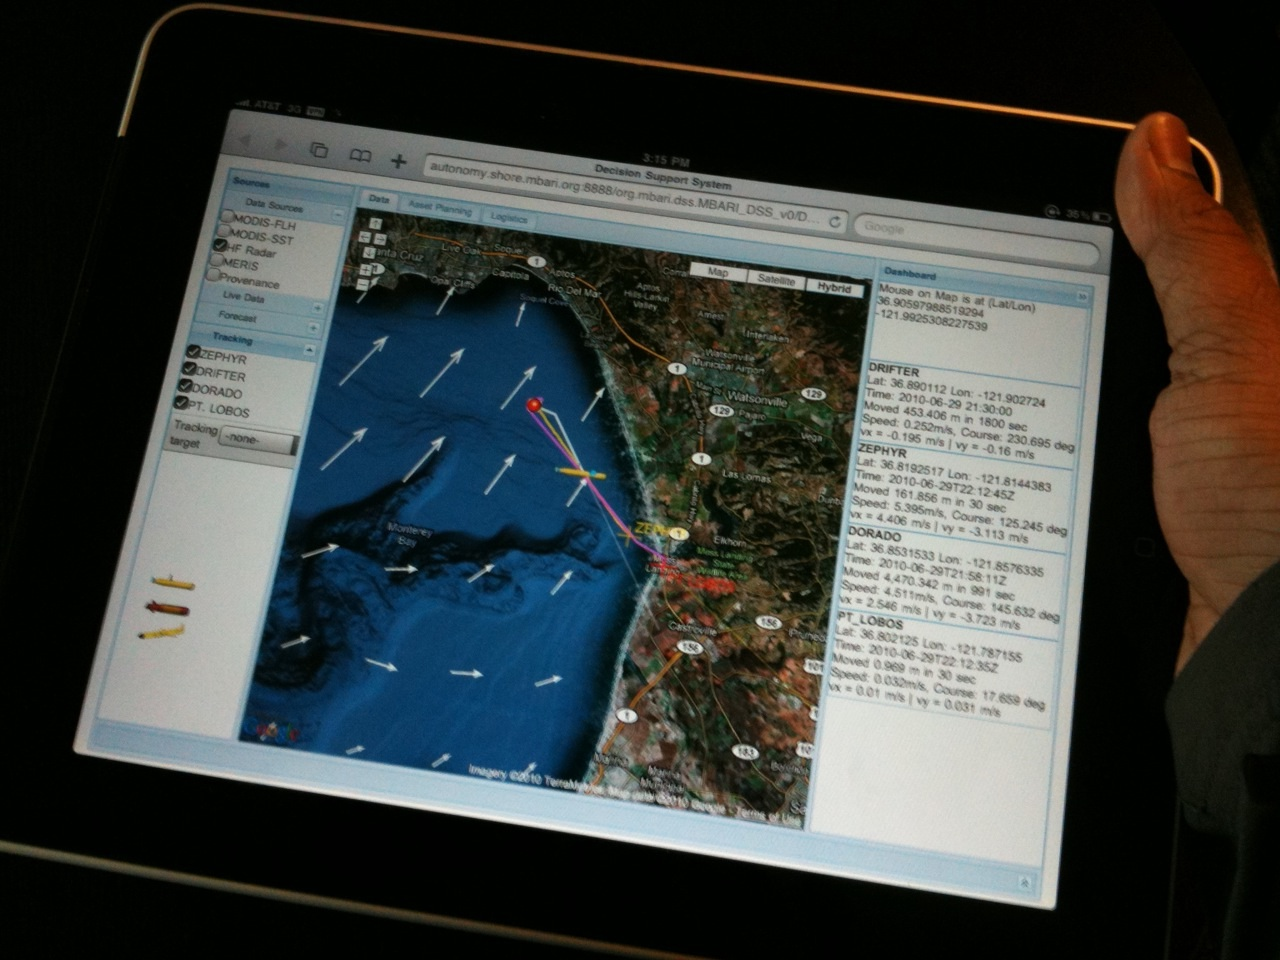
\includegraphics[width=0.3\textwidth]{figs/photo-ipad-2.jpg}}
\caption{\small \ref{fig:odss-mtg} shows a 2010 \can meeting with the
  \od in use. \ref{fig:odss-virtual} shows a drifter tracking tool
  used during \can planning; it used a physical model of advected
  surface currents from \texttt{CeNCOOS} \cite{cencoos} to plan AUV
  deployments. \ref{fig:odss-ipad} shows \od use on an iPad.}
\label{fig:odss2}
\end{figure*}


These distinctions make some vehicles more or less suitable to address
certain science goals and suggest some degree of intelligent planning
in the assignment strategy. Further, even if partial plans can be
synthesized automatically, the need to capture qualitative 'intent'
and desires in the final outcome of an asset allocation strategy
drives us towards a human-in-the-loop approach for asset
allocation. The vast uncertainty and complex interaction between
unknown quantities in the ocean environment dictate that any
comprehensive experimental methodology must rely in some measure on
human reasoning and adaptability.  Furthermore, the multidisciplinary
nature of ocean experiments suggests collaboration between multiple
human actors. Human cognitive capability then to capture these
uncertainties, evaluate options, factor intent and synthesize data
needed for asset allocation becomes increasingly important. Therefore,
mixed-initiative approaches are viable as a means to apportion problem
solving and inference between human and computational approaches. A
viable example was shown in the command and control of the twin Mars
rovers in \cite{aichang04,bresina05,bresina05a}\footnote{The MAPGEN
  system uses the same \eu planner used in \rxe. It continues to be
  used routinely to this day on the MER mission.}.

Additionally, our work on \od is driven by a vision of how marine
field robotics will likely be conducted in the future and the
necessary computational infrastructure that will augment decision
making, onshore as well as on-board. We believe ultimately \od will
combine capabilities inferential and data gathering and analysis
capabilities and more uniquely, provide an event response capability
that could trigger the deployment of a robot and/or adapt its sampling
strategy, all from a scientist's desktop on shore. Data returned from
robotic assets at sea will be filtered for signals associated with
feature(s) of interest along with information on its contextual
environment. The association between the signal and a prospective
event will be undertaken through tagging by experts and machine
learning techniques used in recommender systems
\cite{Adomavicius05}. Adaptive sampling strategies will then balance
decision-making \situ with that done onshore with computational models
and human agents, the subject of a new NSF project in which the
authors are participating.


Operationally, the \od has become a software system that the
scientist consults during a \can field campaign. S/he consults
up-to-date model outputs, synoptic views of ocean color from remote
sensing data and weather conditions for the next $24$-hour planning
cycle and then queries the system to compute candidate sampling
locations. In the near future, the \od will consult its situational
awareness database, incorporate model outputs projecting these outputs
into the space-time region of interest to generates candidate
hypotheses with associated utility metrics. With the scientist's
guidance the automated planner would then determine the most viable
robotic option(s) to be dispatched (underwater, surface or aerial),
given available resources, distance of travel, required payload and
the environment. For instance, unpowered autonomous gliders would be
chosen for longer-duration missions with smaller payload requirements
in areas of moderate to weak ocean currents. The automated planner
would balance these criteria to compute a viable trajectory plan for
the selected vehicle. Vehicles with more controllability would be
given a specified area to survey and the path generated \situ. Goals
are communicated to the robot after analysis on shore for selective
targeting of features by the conglomerate of vehicles in the ocean
being tracked by the \od. Thus far, the \od has provided a simple
yet functional tool for scientists to use in the daily complex
decision making and the following experiment and survey design
needs. It has helped train scientists to think of expanding their
repertoire of tools for the scientific process and in the process it
enabled a mixed team of engineers and scientists to interact at the
functional level of the systems' capabilities.

%%% Local Variables: 
%%% mode: latex
%%% TeX-master: "setobook"
%%% End: 


\section{Future Work}
\label{sec:future}

Our experience of using deliberative techniques in a highly
inter-disciplinary environment for targeted marine science
applications has shown the need and applicability of such novel
algorithms and methods. In addition to augmenting traditional AUV
surveys more advanced Lagrangian observations, mixed-initiative
methods, our colleagues at MBARI have understood the longer term
implications of our work. Our current and consequently future efforts
are therefore grounded in important science problems in an operational
oceanographic setting.

\begin{figure}[h]
  \centering
  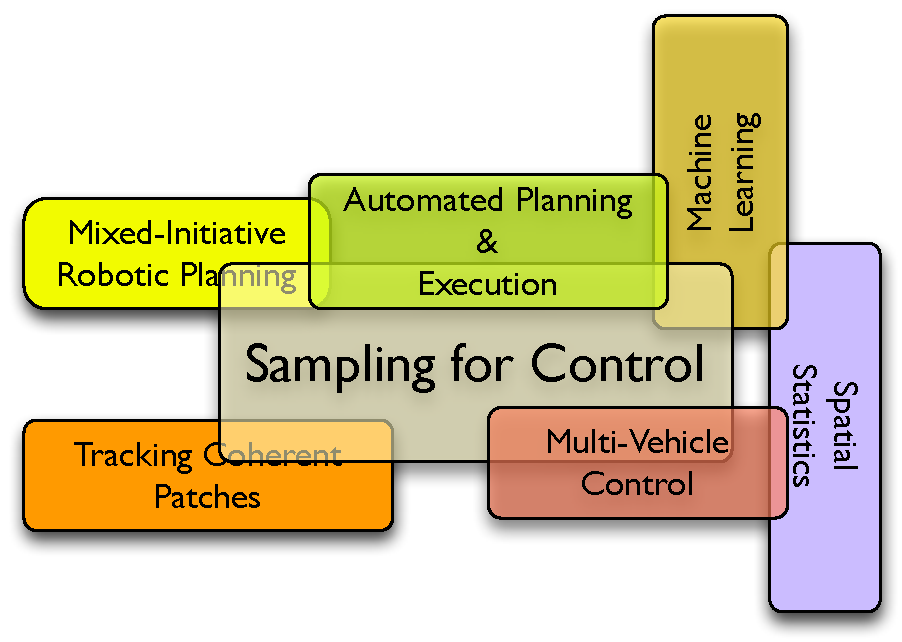
\includegraphics[scale=0.45]{figs/autonomy-topics.pdf}
  \caption{\small Overlapping topics in our research in deliberation
    and autonomy with sampling the dominant theme.}
  \label{fig:topics}
\end{figure}

The core of our problem domain for \can has been towards Sampling. In
large part given the spatial and temporal scales of the
bio-geochemical processes we are interested in in this project, it is
imperative that a key direction is in formulating a multi-robot
adaptive sampling problem. In this context while superficially \rx can
be considered as a multi-agent system and could therefore imply a
direct extension, sporadic communication with high-latencies in
surface communication, not to mention low throughput acoustic
communications imply that the extension of \rx for distributed
applications is non-trivial. Further, in order to efficiently execute
coordinated observation of ocean processes with multiple autonomous
sensing platforms, significant methodological as well as technical
challenges must be addressed. We are working towards a systematic
approach of using \rx as a backend planner for \can field
experiments. The expectation is that \od users will plan initially
individual vehicle surveys which are variants of standard
straight-line transects. Lessons learned with human planners in the
loop will be used towards planning larger surveys, also with simple
fixed transects but using vehicle capabilities in ontologies similar
to \cite{patron09}. Apportioning the planning task between shore-side
components with substantial contextual information and compute power
with robots with in-situ reasoning capabilities a la \rx is a
challenge and an open research problem. Fig. \ref{fig:topics} shows
what we believe is the scope and influence of the different topic
areas we are focusing on.

Partitioned inference and decision-making within \rx also lends itself
to graceful system degradation, making the overall approach effective
towards increased robustness. There are two outstanding diagnosis and
failure recovery challenges that we need to address; the first has to
do with methodology related to model design of the instrument payload
for a highly modular and configurable vehicle; this is local to a
reactor. Doing so would enable (as a first step) using systematic
Fault Diagnosis, Isolation and Recovery (FDIR) algorithms as
demonstrated in the \texttt{RAX} experiment
\cite{williams96,mus98,williams97} and more recently on an AUV by
Dearden and others \cite{wang09,ernits10,dearden11}. The second
challenge has to implementing a policy within the \rx framework that
explicitly deals with recovery since controller failure can be
distributed across reactors. Since reactors are hierarchical in their
relationship to one another, their well defined dependencies allow
them to be removed from an agent systematically. Reactors more
abstract in scope can be removed before those which are less abstract
(and closer to the hardware). In the event a Navigation reactor, for
example, has a fault, it can be removed safely with lower level
functionalities (such as those in the executive). When the Navigator
is removed, it will recursively remove more abstract reactors (such as
a Mission Manager) that depend on it. Such a safety feature then
allows the system designers to ensure that early on they can invest
more in ensuring that reactors lower in the hierarchy are robust and
potentially formally verified. It also means that there is a safe and
sure way to take control of the vehicle at any level within the
reactors hierarchy; as long as low level reactors are still active one
will always been able to send goals/commands to them and execute what
are traditionally known as runout sequences (or clean up scripts).

Feature recognition for Sampling is a general research thrust; however
it has specific relevance in the context of \rx and AUV control. As
noted in Section \ref{sec:results} we have already demonstrated
Machine Learning techniques for recognition of select features in the
coastal ocean. A principal challenge that remains is that of obtaining
expert labeled data for any supervised or semi-supervised learning
methods.  While supervised techniques for learning classifiers such as
decision trees (\cite{Quinlan93-dtrees}), instance-based
classification (\cite{Aha-ibl-ml91}), Bayesian classifiers
(\cite{Jensen2001-BNetworks}) and artificial neural networks
(\cite{ANNsurvey-2000}) are popular, given the vast amount of data
available and poor understanding of correlation between physical and
biogeochemical variables in the coastal ocean, our work on INLs
\cite{mcgann08d,ryan10} and reliance on a oceanographic expert has
shown that scaling to different problems remains problematic. This is
a prime motivation to move towards more semi-supervised methods such
as \cite{kumar11,sergio12}. With the advent of the \od however,
another direction our research is taking us is in \texttt{Recommender
  Systems} \cite{Adomavicius05} as noted in Section
\ref{sec:results}. We are working to design and deploy software
infrastructure that will learn from user tagged data. To do so, we
will use tagging techniques similar to what users of commercial image
sharing sites like Flickr and Picassa do, to learn the context of the
data (including remote sensing). In addition, the \od will integrate
statistical Machine Learning techniques with incoming asynchronous
data stream obtained by sensors and platforms. Identification models
will be based on existing training sets for INLs and plumes; models
for other features of scientific interests driven by \can requirements
will be built in addition. Existing AUV archives for instance provide
sufficient data for a learning base for a range of features of
interest to \can; in addition we will build software that will learn
to incorporate incoming data streams to provide an existence proof of
a feature of interest.

A number of issues remain to be explored improving \rx and \eu
integration particularly in the context of engineering models for
execution.

Dispatchability of the {\em external} temporally flexible partial
plans continues to be an open research problem. Substantial progress
has been made \cite{vidal97,mus98a,tsam98,morris00} by analyzing the
plan structure of static offline temporal plans. However in the
context of embedded plan execution, balancing model design while
dealing with execution uncertainty requires further research. For
instance it should be possible to distinguish part of the plan that
contributes to a reactor goal, which often needs to be dispatched as
early as possible with other tokens describing world evolution with a
preference to dispatch as late as possible. Making this distinction
would improve the quality of agent behavior while avoiding extra model
complexity.

More abstractly at the architectural level, the ability to dynamically
manipulate the reactor graph would be of importance while creating new
reactors or modifying timelines. Doing so would provide more robust
failure recovery mechanisms especially after a reactor has failed to
synchronize. For example, an alternate reactor could take ownership of
timelines left invalid by the destruction of another failed reactor
ensuring a transparent implementation of component redundancy. While
the current design broadly provides for such a capability, the \rx API
has yet to implement it while ensuring other design elements within
\rx and \eu are not compromised.

Finally and importantly, integration of reasoning about resources
within \rx and tying it to existing \eu capabilities needs to be
demonstrated. Specifically \rx needs to be able to update resource
levels as incoming observations.  Doing so would ensure plan
adaptation occurs dynamically when planned and observed resource
values diverge -- for instance if the vehicle looses a bank of
batteries during the course of a mission.  Enhanced modeling
capabilities and augmented domain-independent search within \eu would
make it easier for \rx users to create such domain models and to
perform more proactive deliberation.

Along with all these potential extensions, we are also very cognizant
that the learning curve associated with \rx and \eu for a general user
in the marine robotics community needs to be tackled. At present, the
complex system that underlies \rx and its underlying framework, even
if well documented, can be intimidating for a naive first time user.

% multi-vehicle control
% sampling
% diagnosis and recovery
% feature recognition
% scalable architecture for missions





%%% Local Variables: 
%%% mode: latex
%%% TeX-master: "setobook"
%%% End: 


\section{Conclusion}
\label{sec:conclusion}

% Final parting words summarizing the contribution of deliberation towards
% vehicle autonomy.

The Ocean Sciences are at a cusp, straddling traditional ship-based
exploration with newer observatory-based methods. In the United States
the NSF funded Ocean Observatories Initiative \cite{ooi} and regional
bodies such as \texttt{CeNCOOS} \cite{cencoos} are investing in new
observational methods and technologies which \kcomment{aim} to aid
oceanographers by producing substantially higher-resolution data
products. These will use moorings, cabled observatories and glider
fleets generating near real-time data from one or more locations as a
continuous stream. The tack chosen by \can has been to complement such
methods with the aim of developing methods for a \emph{portable
  mobile} observatory which is dependent on autonomous platforms. In
this context what we advocate in this chapter is an initial step in
making robotic platforms more adaptive, scaling them towards fleets of
vehicles (underwater \kcomment{and/}or on the surface) and most
importantly using them to solve the larger challenge of sampling
\kcomment{dynamic} spatio-temporal fields.

While our trajectory of research in the oceanographic domain follows
that in spacecraft autonomy, from onboard \cite{mus98} to
mixed-initiative methods \cite{bresina05}, the challenges are
significantly different with the environment playing a far larger
role. Moreover, prediction and projection of a future course of action
for a robot given the level of uncertainty calls for representational
and architectural methods which would enable adaptation at different
levels of abstraction, from mission-planning to low level actuation
\kcomment{and control}.

Our efforts were initially targeted to full robotic autonomy; while
this is an important goal that we continue to strive towards, it is
increasingly clear that human-in-the-loop methods also have a sizable
role to play in ocean exploration and by extension to \kcomment{the
  field of} Marine Robotics. Not only is an embedded
\kcomment{deliberative agent} an important element of the effort
towards smarter vehicles, but we are working towards an implementation
of \rx which will perform multi-vehicle plan synthesis for the \ode.

A key role that \rx has played and will continue to play, is towards
\emph{event response} scenarios. In Section \ref{sec:results} we show
the role Machine Learning techniques have played thus far in in-situ
plan adaptation. This interaction between Planning and Machine
Learning, we believe, will play a significant role going forward in
exploration and discovery. Interpretation of incoming sensor data to
deal with scientific surprise and \kcomment{re-adaptation} for
opportunistic science will be critical to dealing with the persistent
problem of undersampling the ocean\footnote{Walter Munk of the Scripps
  Institute of Oceanography has famously stated \emph{``Most of the
    previous century could be called a “century of undersampling”''}
  -- Testimony to the U.S. Commission On Ocean Policy, 18 April
  2002}. 

Much of what we know of the ocean was derived by exploring in the
blind. In the near future, we anticipate longer duration robotic
vehicles with enough onboard computational capacity to run
deliberative agents such as \rxe, make water-column measurements and
reliably track and characterize dynamic features. While our
\kcomment{own} experiments have already demonstrated such
capabilities, the exploration Vs. exploitation tradeoff is better
determined when vehicles can make choices over longer time periods
(weeks and months) to study the impacts of bio-geochemical interaction
driven by longer duration physical forcing \kcomment{and climate
  change}.

Given our poor understanding of the coastal ocean in particular,
mixed-initiative methods of command and control for Sampling with
heterogenous assets is an important goal that is clearly at our
doorstep. We believe deliberation is, but a small yet critical part of
the solution to unfolding open research problems for AI and Marine
Robotics.


\section{Acknowledgements}

Rajan and Py are funded by a block grant from the David and Lucile
Packard Foundation to MBARI. They thank their collaborators John Ryan,
Julio Harvey, Jim Bellingham and Robert Vrijenhoek at MBARI. In
addition they thank colleagues Martha del Alto, David Korsmeyer and
Steven Zornetzer at NASA Ames who made \eu available as open
source. The authors thank other members of the \eu team over the
years, including Ari J\'onsson, Jeremy Frank, Conor McGann, Paul
Morris, Michael Iatauro, Matthew Boyce and Tristan Smith.  Minh Bin Do
(NASA Ames), William Yew Teck Tan (NUS, Singapore) and Rishi Graham
(MBARI) provided comments on early drafts; we are grateful for their
help in making this manuscript more accessible. Finally, the authors
are indebted to Nicola Muscettola for his ideas and early efforts in
Constraint-based Temporal Planning at NASA Ames which forms the basis
of much of this work.

\bibliographystyle{IEEEtran}
\bibliography{references}

\end{document}
